% !TEX root = ../PDE4ML.tex

\section{Wasserstein Gradient Flows}
\index{Wasserstein gradient}% strictindex
\index{gradient!flow}% strictindex
\index{Wasserstein!gradient flow}% strictindex
\label{sec-wasserstein-gradient-flows}

Once dynamic transport gives a metric on measures, one can run gradient descent directly on probability laws. This section follows the current OT4ML treatment while emphasizing the PDE/ML mechanisms: JKO schemes, Wasserstein gradients, geodesic convexity, functional inequalities, mean-field neural-network training, generalized transport geometries, conditional ResNets and inertial particle flows.\index{JKO scheme}% strictindex
\index{mean-field neural network}% strictindex
\index{functional inequality}% strictindex

\subsection{Minimizing Movements and Wasserstein Gradients}
\index{minimizing movement}% strictindex
\index{Wasserstein gradient}% strictindex

This first section explains how a variational implicit-Euler step on measures gives rise, in the small-step limit, to a continuity equation driven by the Wasserstein gradient of the energy.
\index{continuity equation}% strictindex

We now consider a function $f(\alpha)$ and seek a minimizing evolution $(\alpha_t)_t$. The general strategy of minimizing movement over a metric space is to construct a discrete-time evolution using an implicit Euler scheme:
\index{implicit Euler scheme}% strictindex
\begin{equation}
    \alpha_{t+\tau} := \arg\min_\alpha \frac{1}{2 \tau} \Wass_2(\alpha_t, \alpha)^2 + f(\alpha). \label{eq:jko-discr}
\end{equation}

\begin{alg}[JKO minimizing movement]\label{alg:jko-minimizing-movement}
\index{JKO scheme}% strictindex
\textbf{Input:} Energy $f$, initial measure $\alpha^0$, time step $\tau>0$, number of steps $K$.

\textbf{Output:} Discrete gradient-flow trajectory $(\alpha^k)_{k=0}^K$.

\textbf{For} $k=0,\ldots,K-1$ \textbf{do}:
\begin{algblock}
\(\alpha^{k+1} \in \uargmin{\alpha\in\Pp_2(\RR^d)} \frac{1}{2\tau}\Wass_2^2(\alpha^k,\alpha)+f(\alpha).\)

\textbf{Set} $\alpha_t^\tau=\alpha^k$ for $t\in[k\tau,(k+1)\tau)$.

\end{algblock}
\algreturnskip
\textbf{Return} $(\alpha^k)_{k=0}^K$ and $\alpha_t^\tau$.
\end{alg}

\paragraph{Euclidean gradient flows.}
\index{gradient!flow}% strictindex

If we restrict \eqref{eq:jko-discr} to finite dimensions and assume $\alpha_t = \delta_{x(t)}$ and $\alpha = \delta_x$ (single Dirac measures), this matches the implicit Euler scheme:
\index{Dirac mass}% strictindex
\index{implicit Euler scheme}% strictindex
\begin{equation*}
    x(t+\tau) := \arg\min_x \frac{1}{2 \tau} \norm{x - x(t)}^2 + h(x),
\end{equation*}
where $h(x) = f(\delta_x)$. Its solution is formally given by the implicit Euler formula:
\begin{equation*}
    x(t+\tau) = (\Id + \tau \nabla h)^{-1}(x(t)).
\end{equation*}
In contrast, the explicit Euler scheme is:
\begin{equation*}
    x(t+\tau) = (\Id - \tau \nabla h)(x(t)) = x(t) - \tau \nabla h(x(t)).
\end{equation*}

Both schemes converge as $\tau \to 0$ to:
\begin{equation}
    \dot{x}(t) = -\nabla h(x(t)). \label{eq:grad-flow-classical}
\end{equation}


\paragraph{Wasserstein gradient formula.}
\index{Wasserstein gradient}% strictindex

The implicit Euler scheme has the advantage that it does not require $h$ or $f$ to be smooth. For $f$, this is crucial to handle evolutions over measures that may have densities, atoms or other singular parts.
\index{implicit Euler scheme}% strictindex

As $\tau \to 0$, under certain conditions on $f$, \eqref{eq:jko-discr} defines a continuous evolution $t \mapsto \alpha_t$. As discussed earlier, this evolution can be described as a Lagrangian evolution \eqref{eq:lagrangian-advection}. We use the following first-variation convention: for any $\beta\in\Pp(\RR^d)$ and the signed zero-mass perturbation $\rho=\beta-\alpha$,
\index{first variation}% strictindex
\index{signed!measure}% strictindex
\begin{equation*}
    f((1-\tau)\alpha + \tau \beta) = f(\alpha + \tau \rho) = f(\alpha) + \tau \int [\delta f(\alpha)](x) \d \rho(x) + o(\tau).
\end{equation*}
The key infinitesimal object is the vector field that represents this differential in the Wasserstein metric.

\Needspace{7\baselineskip}
\begin{defn}[Wasserstein gradient]\label{def-wasserstein-gradient}
\index{Wasserstein gradient}% strictindex
	Assume that $f$ admits a smooth first variation $\delta f(\alpha)$. In the smooth formal calculus on $\Pp_2(\RR^d)$, the Wasserstein gradient of $f$ at $\alpha$ is the gradient vector field
	\begin{equation*}
	    \Wgrad f(\alpha) = \nabla_x \delta f(\alpha).
	\end{equation*}
\end{defn}
The associated formal gradient flow is the continuity equation
\begin{equation}
    \frac{\partial \alpha_t}{\partial t} + \diverg(-\Wgrad f(\alpha_t) \alpha_t) = 0. \label{eq:wassflow-pde}
\end{equation}
The following proposition explains why this vector field is the Riemannian gradient for the $L^2(\alpha)$ metric on velocities.
\index{signed!measure}% strictindex
%
\begin{proposition}[Formal Wasserstein gradient]\label{prop-formal-wass-gradient}
\index{Wasserstein gradient}% strictindex
	Assume that $f$ admits a smooth first variation $\delta f(\alpha)$ and that $\alpha$ has a smooth positive density. For infinitesimal perturbations generated by a velocity field $v$ through $(\Id+\tau v)_\sharp\alpha$, the differential of $f$ is
\index{first variation}% strictindex
\index{velocity field}% strictindex
	\[
		\frac{\d}{\d\tau}_{|\tau=0}
		f\big((\Id+\tau v)_\sharp\alpha\big)
		=
		\int \dotp{\nabla \delta f(\alpha)(x)}{v(x)}\d\alpha(x).
	\]
	Hence, for the Riemannian metric $\norm{v}_{L^2(\alpha)}^2=\int \norm{v}^2\d\alpha$, the Wasserstein gradient is the vector field
\index{Wasserstein gradient}% strictindex
	\[
		\Wgrad f(\alpha)=\nabla \delta f(\alpha).
	\]
\end{proposition}
\begin{proof}
	The push-forward expansion gives, in the sense of distributions,
\index{push-forward}% strictindex
	\[
		(\Id+\tau v)_\sharp\alpha
		=
		\alpha-\tau\diverg(\alpha v)+o(\tau).
	\]
	Using the definition of the first variation,
\index{first variation}% strictindex
	\[
		f((\Id+\tau v)_\sharp\alpha)
		=
		f(\alpha)-\tau\int \delta f(\alpha)\diverg(\alpha v)\d x+o(\tau).
	\]
	An integration by parts, with either compact support or vanishing boundary flux, gives
\index{flux}% strictindex
	\[
		-\int \delta f(\alpha)\diverg(\alpha v)\d x
		=
		\int \dotp{\nabla\delta f(\alpha)}{v}\d\alpha.
	\]
	By definition of the Riesz representative for the $L^2(\alpha)$ metric, this representative is $\nabla\delta f(\alpha)$.
\end{proof}

The Wasserstein gradient-flow viewpoint already appears in John D. Lafferty's PhD work, published as ``The Density Manifold and Configuration Space Quantization'', under the name ``density manifold''. It was then systematically developed by Otto, who exposed the formal Riemannian structure of this space~\cite{otto2001geometry}. Rigorous metric-space treatments and numerical JKO schemes can be found in~\cite{ambrosio2006gradient,JDB-JKO,2015-Peyre-siims,gallouet2017jko}.
\index{Wasserstein gradient}% strictindex
\index{Wasserstein!gradient flow}% strictindex
\index{JKO scheme}% strictindex

%%%%
\paragraph{From the JKO step to the velocity field.}
\index{velocity field}% strictindex

A first-order expansion of the JKO step explains why~\eqref{eq:wassflow-pde} uses the vector field $\Wgrad f(\alpha)$. Write \eqref{eq:jko-discr} as a minimization over displacement fields $v$ such that $\alpha = (\Id + \tau v)_\sharp \alpha_t$:
	\[
		\min_{v} \frac{1}{2 \tau} \tau^2 \norm{v}_{L^2(\alpha_t)}^2 + f( (\Id + \tau v)_\sharp \alpha_t ).
	\]
Then we perform a first-order Taylor expansion of this formulation using
	\[
		 (\Id + \tau v)_\sharp \alpha_t =  \alpha_t - \tau \diverg( v \alpha_t ) + o(\tau)
	\]
	\[
		f( (\Id + \tau v)_\sharp \alpha_t ) = f(\alpha_t) - \tau \int \delta f(\alpha_t) \diverg( v \alpha_t ) \d x + o(\tau)
	\]
	\[
		 = f(\alpha_t) + \tau \int \langle \nabla_x \delta f(\alpha_t)(x), v(x) \rangle \d \alpha_t(x) + o(\tau)
	\]
to obtain the following first-order expansion in $\tau$ of the problem minimized in \eqref{eq:jko-discr}
	\[
		 \min_{v} f(\alpha_t) +  \tau \int \Big[ \frac{1}{2} \norm{v(x)}^2 + \langle \Wgrad f(\alpha_t)(x), v(x) \rangle \Big]\d \alpha_t(x) + o(\tau).
	\]
The pointwise minimizer is $v=-\Wgrad f(\alpha_t)$, which gives the velocity in the continuity equation.
\index{continuity equation}% strictindex

\paragraph{Metric derivative and curves of maximal slope.}
\index{metric derivative}% strictindex
\index{curve of maximal slope}% strictindex
\index{slope!metric}% strictindex
\index{local metric slope}% strictindex

The same descent principle admits a coordinate-free formulation, which is the right language for limits of JKO schemes. Let $(\mathcal X,d)$ be a metric space and let $x:(0,T)\to\mathcal X$ be an absolutely continuous curve. Its metric derivative is
	\[
		|\dot x_t|
		\eqdef
		\lim_{h\to 0}\frac{d(x_{t+h},x_t)}{|h|}
	\]
for a.e. $t$. Equivalently, $|\dot x_t|$ is the smallest $g\in L^1_{\rm loc}(0,T)$ such that $d(x_s,x_t)\leq \int_s^t g(r)\d r$ for all $0<s<t<T$. If $f:\mathcal X\to(-\infty,+\infty]$ is lower semicontinuous, its local metric slope at a point $x$ with $f(x)<+\infty$ is
	\[
		|\partial f|(x)
		\eqdef
		\limsup_{\substack{y\to x\\ y\neq x}}
		\frac{( f(x)-f(y) )_+}{d(x,y)} .
	\]
When this slope is a strong upper gradient for $f$, meaning that $|f(y_t)-f(y_s)|\leq \int_s^t |\partial f|(y_r)|\dot y_r|\d r$ along absolutely continuous curves $y_r$, an absolutely continuous curve $x_t$ is called a curve of maximal slope if it satisfies the energy-dissipation inequality
\index{strong upper gradient}% strictindex
\index{energy-dissipation inequality}% strictindex
	\[
		f(x_t)
		+\frac12\int_s^t |\dot x_r|^2\d r
		+\frac12\int_s^t |\partial f|^2(x_r)\d r
		\leq f(x_s),
		\qquad 0\leq s<t.
	\]
This is the metric-space formulation of gradient descent~\cite{ambrosio2006gradient}; the inequality is stable under weak limits, while in smooth Hilbert or Wasserstein settings it is usually saturated. In $\mathcal X=\Pp_2(\RR^d)$ with $d=\Wass_2$, an absolutely continuous curve admits a continuity-equation velocity $v_t$ and satisfies $|\dot\alpha_t|_{\Wass_2}\leq\norm{v_t}_{L^2(\alpha_t)}$, with equality for the minimal velocity. For smooth energies, $|\partial f|(\alpha_t)=\norm{\Wgrad f(\alpha_t)}_{L^2(\alpha_t)}$, so the maximal-slope condition reduces to the velocity-field equation $v_t=-\Wgrad f(\alpha_t)$ derived above. The energy consequences of this viewpoint are used below in Section~\ref{sec-geodesic-convexity}.
\index{minimal velocity}% strictindex

We now detail examples of such Wasserstein gradient flows.
\index{Wasserstein gradient}% strictindex
\index{gradient!flow}% strictindex
\index{Wasserstein!gradient flow}% strictindex

\begin{example}[Application to single-cell gradient-flow models]\label{ex-single-cell-gradient-flow}
\index{single-cell genomics}% strictindex
\index{Waddington landscape}% strictindex
	Instead of only coupling successive snapshots, one may posit that a latent population law evolves by
	\[
		\partial_t\al_t+\diverg(\al_t v_t)=0,
		\qquad
		v_t=-\Wgrad f(\al_t)=-\nabla\delta f(\al_t).
	\]
	Here \(\delta f(\al_t)\) is the first variation, with the convention introduced above. For example, if \(\al=\rho\,\d x\), the energy \(f(\al)=\int V\d\al+\tau\int\rho\log\rho\,\d x\) gives a drift toward a potential landscape \(V\) together with diffusion. In single-cell modeling, \(V\), interaction terms or a neural approximation of \(v_t\) can be fitted from unpaired population snapshots. This links Waddington-landscape intuition to the mathematical language of dynamic OT, Fokker--Planck equations and flow matching~\cite{TongHuangWolfVanDijkKrishnaswamy2020TrajectoryNet,LavenantZhangKimSchiebinger2021TrajectoryInference,KleinUsciddaTheisCuturi2023GENOT}.
\end{example}

\begin{figure}[H]
\centering
\begin{tabular}{@{}cc@{}}
\small density iterates & \small quantile motion \\[-.15em]
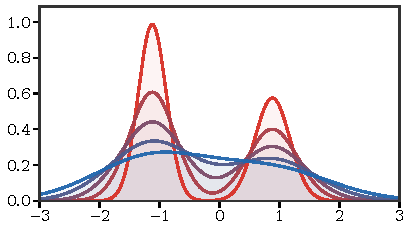
\includegraphics[width=.43\linewidth]{figures/gradflow-jko-entropy-steps/density-steps.pdf} &
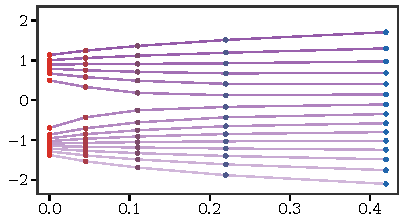
\includegraphics[width=.43\linewidth]{figures/gradflow-jko-entropy-steps/quantile-steps.pdf}
\end{tabular}
\caption{\emph{JKO minimizing movements for the entropy flow in one dimension.} The left panel displays successive implicit-Euler minimizers for the heat equation, colored from red to blue. The right panel tracks inverse CDF values $Q_t(s)=F_t^{-1}(s)$ for selected probability levels $s$, giving a Lagrangian view of the proximal movement in Wasserstein space.}
\index{minimizing movement}% strictindex
\index{Wasserstein!space}% strictindex
\index{heat equation}% strictindex
\index{JKO scheme}% strictindex
\label{fig:gradflow-jko-entropy-steps}
\end{figure}

%%%
\paragraph{Discrete evolutions.}
\index{measure!evolution}% strictindex

If $f(\alpha)$ can be evaluated on discrete distributions and $\Wgrad$ is continuous in this case, the flow \eqref{eq:wassflow-pde} maintains the number of Dirac masses, $\alpha_t = \frac{1}{n} \sum_i \delta_{x_i(t)}$. The particles $X(t) := (x_i(t))_i$ evolve according to a system of coupled ODEs:
\index{Dirac mass}% strictindex
\begin{equation}
    \dot{x}_i(t) = -n\nabla_{x_i} F(X(t)), \label{eq:wassflows-particles}
\end{equation}
where $F(X) := f\left(\frac{1}{n} \sum_i \delta_{x_i}\right)$ and the factor $n$ comes from the empirical Wasserstein metric $\frac1n\sum_i \norm{\dot x_i}^2$.

\begin{alg}[Empirical Wasserstein particle descent]\label{alg:empirical-wasserstein-particle-flow}
\index{particle Wasserstein descent}% strictindex
\textbf{Input:} Particles $X^0=(x_1^0,\ldots,x_n^0)$, functional $f$, step size $h$, tolerance $\mathrm{tol}$.

\textbf{Output:} Particle trajectory $(X^k)_k$ and empirical measures.

\textbf{Define}
\(F(X)=f\!\left(\frac1n\sum_{i=1}^n\delta_{x_i}\right).\)

\textbf{For} $k=0,1,\ldots$ \textbf{do}:
\begin{algblock}

\textbf{For} $i=1,\ldots,n$ \textbf{do}
\begin{algblock}
\(g_i^k=n\nabla_{x_i}F(X^k), \qquad x_i^{k+1}=x_i^k-h\,g_i^k.\)
\end{algblock}
\textbf{If} \(\max_i\norm{x_i^{k+1}-x_i^k}\leq \mathrm{tol}\) \textbf{then}:
\begin{algblock}
\textbf{Return} $\frac1n\sum_i\delta_{x_i^{k+1}}$.
\end{algblock}
\end{algblock}
\end{alg}

%%%
\paragraph{Linear Functionals.}
\index{linear!functional}% strictindex

The first benchmark is a functional whose first variation does not depend on the current measure.

\begin{example}[Linear potentials generate independent particles]
Take a linear functional
   \begin{equation}\label{eq:linear-func}
       f(\alpha) = \int h(x) \d \alpha(x).
   \end{equation}
   Then $\delta f(\alpha) = h$ is independent of $\alpha$, and the flow \eqref{eq:wassflow-pde} becomes
   \begin{equation*}
       \frac{\partial \alpha_t}{\partial t} + \diverg(-\nabla h \alpha_t) = 0.
   \end{equation*}
   This implies particles move independently according to the usual gradient flow \eqref{eq:grad-flow-classical}.
\index{gradient!flow}% strictindex
\end{example}

%%%
\paragraph{Shannon Neg-Entropy.}
\index{negative Shannon entropy}% strictindex


Entropy gives the opposite benchmark: the flow is no longer a deterministic push-forward of particles, but a diffusion of density.

\begin{example}[Entropy generates heat and porous-medium flows]
The canonical density-dependent functional is the Shannon neg-entropy
   \begin{equation}
       f(\alpha) = \int \log\left(\frac{\d \alpha}{\d x}(x)\right) \d \alpha(x). \label{eq:entropy-func}
   \end{equation}
   Here, $\delta f(\alpha) = \log(\d\alpha/\d x)$ up to an additive constant, so $\Wgrad f(\alpha) = \nabla \alpha/\alpha$ (often called the score). The flow \eqref{eq:wassflow-pde} becomes the heat equation
\index{score function}% strictindex
\index{heat equation}% strictindex
   \begin{equation*}
       \partial_t \alpha_t = \Delta \alpha_t.
   \end{equation*}
   Other entropy functionals lead to nonlinear diffusion equations; finite-volume and particle discretizations are discussed in~\cite{CarrilloFiniteVolume,GianazzaARMA,Maas2011,ErbarHeatManifold}.
%
For a generalized entropy
   \begin{equation}\label{eq:gen-entropies}
       f(\alpha) = \int g\left(\frac{\d \alpha}{\d x}\right) \d x,
   \end{equation}
	   with a scalar convex function $g$, one obtains nonlinear diffusions in the smooth-density regime:
\index{convex!function}% strictindex
   \begin{equation*}
       \frac{\partial \alpha_t}{\partial t} = \Delta(P(\alpha_t)),
   \end{equation*}
   where the pressure $P$ satisfies $P'(s)=s g''(s)$. For example, $g(s) = s \log(s)$ gives $P(s)=s$ and recovers \eqref{eq:entropy-func}, while $g(s) = s^m/(m-1)$, $m > 1$, gives $P(s)=s^m$ up to an additive constant and yields the porous-medium equation.
\index{porous medium equation}% strictindex
\end{example}

\begin{rem}[Two gradient-flow interpretations of the heat equation]\label{rem-two-interpretations-heat-equation}
\index{heat equation}% strictindex
\index{Dirichlet energy}% strictindex
\index{gradient!flow}% strictindex
\index{Shannon entropy}% strictindex
\index{Wasserstein!gradient flow}% strictindex
	The heat equation already illustrates that a PDE does not determine a unique gradient-flow structure. Write $\alpha=\rho\d x$ on a flat domain, with periodic or no-flux boundary conditions. In the Hilbert geometry of densities, the squared distance and the Dirichlet energy are
	\[
		d_{L^2}^2(\alpha,\beta)=\int |\rho_\alpha(x)-\rho_\beta(x)|^2\d x,
		\qquad
		\mathcal D(\alpha)=\frac12\int \norm{\nabla\rho(x)}^2\d x,
	\]
	so $\delta\mathcal D/\delta\rho=-\Delta\rho$ and the $L^2$ gradient flow $\partial_t\rho_t=-\delta\mathcal D/\delta\rho(\rho_t)$ gives $\partial_t\rho_t=\Delta\rho_t$. This viewpoint says that heat flow decreases oscillations and regularizes the density. In Wasserstein geometry, the same equation is instead the $\Wass_2$ gradient flow of the Shannon entropy $\int \rho\log\rho\d x$, so the driving mechanism is entropic spreading. The example is a useful warning: explaining a dynamics as a gradient flow requires specifying both an energy and a metric, and different pairs $(f,d)$ may produce the same PDE.
\end{rem}

\begin{figure}[ht]
\centering
\begin{tabular}{@{}ccc@{}}
\small heat equation & \small porous medium $m=2$ & \small porous medium $m=6$ \\[-.15em]
\index{heat equation}% strictindex
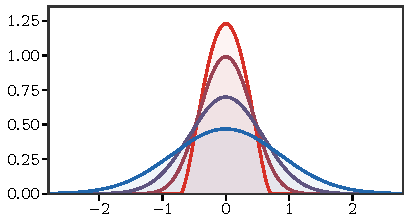
\includegraphics[width=.30\linewidth]{figures/gradflow-heat-versus-porous-medium/heat.pdf} &
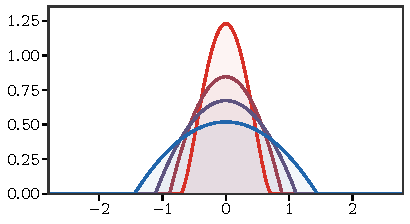
\includegraphics[width=.30\linewidth]{figures/gradflow-heat-versus-porous-medium/porous-medium.pdf} &
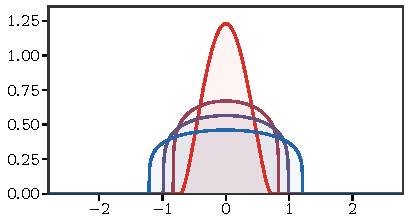
\includegraphics[width=.30\linewidth]{figures/gradflow-heat-versus-porous-medium/porous-medium-m6.pdf}
\end{tabular}
\caption{\emph{Entropy-driven Wasserstein gradient flows from the same compact initial density.} The heat flow is generated by Shannon entropy $g(\rho)=\rho\log\rho$ and instantly develops Gaussian tails. The porous-medium flows use the power entropy $g(\rho)=\rho^m/(m-1)$, hence $\partial_t\rho=\Delta(\rho^m)$: the middle panel has $m=2$, while the right panel has the stronger nonlinearity $m=6$, i.e. $\partial_t\rho=\Delta(\rho^6)$. Larger powers diffuse mainly where the density is high, producing a flatter core and a sharper compact free boundary.}
\index{Wasserstein!gradient flow}% strictindex
\index{Shannon entropy}% strictindex
\label{fig:gradflow-heat-versus-porous-medium}
\end{figure}

%%%
\paragraph{Interaction Energies.}
\index{energy!interaction}% strictindex

In a similar spirit, to obtain nonlinear evolutions without requiring the measure to have density, one can consider
   \begin{equation}
       f(\alpha) := \iint k(x, y) \d \alpha(x) \d \alpha(y). \label{eq:quadratic-func}
   \end{equation}
   For a symmetric kernel $k$:
   \begin{equation*}
       \delta f(\alpha)(x) = 2 \int k(x, y) \d \alpha(y), \quad \Wgrad f(\alpha)(x) = 2 \int \nabla_x k(x, y) \d \alpha(y).
   \end{equation*}
   For $\alpha_0 = \frac{1}{n} \sum_i \delta_{x_i}$, the flow \eqref{eq:wassflow-pde} implies particles $(x_i(t))_i$ obey:
   \begin{equation*}
       \dot{x}_i(t) = -\frac{2}{n} \sum_j \nabla k(x_i(t), x_j(t)).
   \end{equation*}
	   If $k$ is positive definite, or more generally conditionally positive definite on signed measures of zero total mass as for the energy-distance kernel $k(x,y)=-\norm{x-y}$, and one minimizes the squared kernel discrepancy to a teacher distribution $\beta$, then
\index{teacher distribution}% strictindex
\index{energy distance}% strictindex
\index{signed!measure}% strictindex
   \[
       \norm{\alpha-\beta}_k^2
       =
       \iint k\d\alpha\d\alpha
       -2\int\!\left(\int k(x,y)\d\beta(y)\right)\d\alpha(x)
       +\mathrm{constant}.
       \]
	       Thus MMD-type training energies are exactly an interaction energy plus a linear potential; the teacher distribution appears through the potential $x\mapsto-2\int k(x,y)\d\beta(y)$. The corresponding empirical Wasserstein gradient flow is
\index{teacher distribution}% strictindex
\index{Wasserstein gradient}% strictindex
\index{gradient!flow}% strictindex
\index{maximum mean discrepancy}% strictindex
\index{Wasserstein!gradient flow}% strictindex
\index{energy!interaction}% strictindex
       \[
		\dot x_i(t)
		=
		-\frac{2}{n}\sum_j\nabla_x k(x_i(t),x_j(t))
		+
		2\int\nabla_x k(x_i(t),y)\d\beta(y).
       \]

The corresponding simulation loop is Algorithm~\ref{alg:mmd-particle-flow}.

\begin{alg}[MMD particle flow against a teacher law]\label{alg:mmd-particle-flow}
\index{maximum mean discrepancy}% strictindex
\textbf{Input:} Initial particles $(x_i^0)_{i=1}^n$, teacher law $\beta$ or teacher samples $(y_b)_{b=1}^B$, kernel $k$, step size $h$.

\textbf{Output:} Particle trajectory targeting $\beta$.

\textbf{For} $k=0,1,\ldots$ \textbf{do}:
\begin{algblock}

\textbf{For} $i=1,\ldots,n$ \textbf{do}
\begin{algblock}
\textbf{Set} self-interaction \(r_i^k=-\frac{2}{n}\sum_{j=1}^n\nabla_x k(x_i^k,x_j^k)\).

\textbf{If} $\beta$ is available analytically \textbf{then}:
\begin{algblock}

\textbf{Set} teacher attraction \(a_i^k=2\int\nabla_x k(x_i^k,y)\d\beta(y)\).

\end{algblock}
\textbf{If} only samples $(y_b)_{b=1}^B$ are available \textbf{then}:
\begin{algblock}

\textbf{Set} \(a_i^k=\frac{2}{B}\sum_{b=1}^B\nabla_x k(x_i^k,y_b)\).

\end{algblock}
\textbf{Set} velocity \(v_i^k=r_i^k+a_i^k\).

\textbf{Update}
\(x_i^{k+1}=x_i^k+h\,v_i^k.\)
\end{algblock}
\end{algblock}
\algreturnskip
\textbf{Return} $(x_i^k)_{i,k}$.
\end{alg}

	       The first term is a kernelized self-interaction, while the second is the attraction induced by the continuous teacher kernel mean. At the continuum level, characteristic positive-definite kernels, and the Euclidean energy-distance kernel on probability measures, have $\beta$ as the unique minimizer of $\norm{\alpha-\beta}_k^2$. For a finite number of particles, however, the flow can only form a kernelized quadrature of $\beta$, and small particle systems may cover the target modes poorly. Figure~\ref{fig:gradflow-mmd-particle-count} illustrates this finite-particle effect.
\index{kernelized self-interaction}% strictindex
\index{teacher kernel mean}% strictindex
\index{characteristic kernel}% strictindex
\index{kernel quadrature}% strictindex
\index{probability measure}% strictindex
\index{kernel!positive definite}% strictindex
\index{energy distance}% strictindex

\begin{figure}[ht]
\centering
\begin{tabular}{@{}ccc@{}}
\small $n=10$ particles & \small $n=50$ particles & \small $n=300$ particles \\[-.15em]
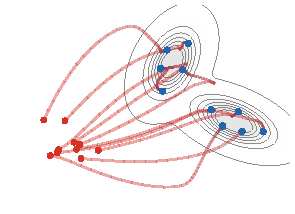
\includegraphics[width=.30\linewidth]{figures/gradflow-mmd-particle-count/n-010.pdf} &
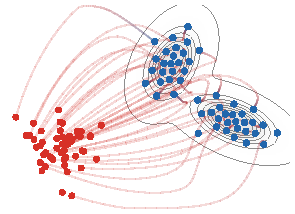
\includegraphics[width=.30\linewidth]{figures/gradflow-mmd-particle-count/n-050.pdf} &
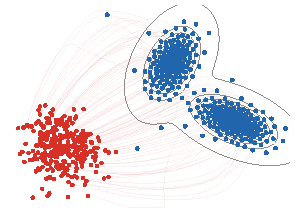
\includegraphics[width=.30\linewidth]{figures/gradflow-mmd-particle-count/n-300.pdf}
\end{tabular}
\caption{\emph{Particle count in an energy-distance Wasserstein particle flow.} The squared MMD-type discrepancy uses the energy-distance kernel $k(x,y)=-\norm{x-y}$ and targets a smooth two-Gaussian teacher distribution. The teacher itself is shown only through true density contours, while red dots are a compact shifted Gaussian initialization placed away from the target, red-to-blue curves show a thinned subset of particle trajectories, and blue dots show the stabilized long-time particles. With too few particles, the empirical measure forms a sparse kernelized quadrature and may under-cover the target modes; increasing $n$ makes the particle cloud approximate the continuous target geometry more faithfully.}
\index{teacher distribution}% strictindex
\index{kernel quadrature}% strictindex
\index{Wasserstein!gradient flow}% strictindex
\index{empirical!measure}% strictindex
\index{energy distance}% strictindex
\label{fig:gradflow-mmd-particle-count}
\end{figure}

The preceding particle flow minimizes a squared kernel discrepancy. Figure~\ref{fig:gradflow-discrepancy-density-comparison} contrasts this with flows generated by three discrepancies toward the same target. For the energy distance and $\Wass_2$, the energy is the unsquared distance, so the Wasserstein velocity is normalized by the current discrepancy value away from the target. The KL case is different: it is a relative-entropy gradient flow and therefore follows the Fokker--Planck diffusion toward the target. The comparison keeps the endpoint fixed and makes the geometry visible through the transient densities.

\begin{figure}[ht]
\centering
\begin{tabular}{@{}ccc@{}}
\small energy distance & \small $\Wass_2$ distance & \small relative entropy \\[-.15em]
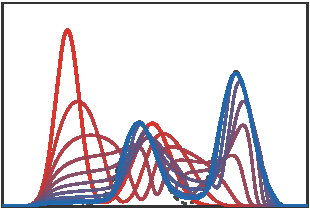
\includegraphics[width=.30\linewidth]{figures/gradflow-discrepancy-density-comparison/energy-distance.pdf} &
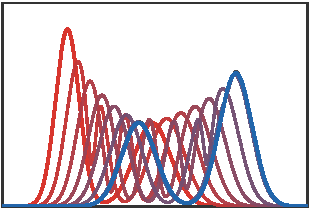
\includegraphics[width=.30\linewidth]{figures/gradflow-discrepancy-density-comparison/w2.pdf} &
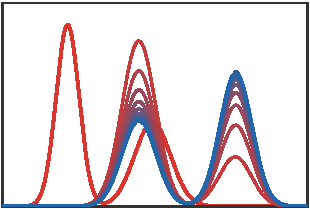
\includegraphics[width=.30\linewidth]{figures/gradflow-discrepancy-density-comparison/kl.pdf}
\end{tabular}
\caption{\emph{Wasserstein gradient flows of three discrepancies toward the same one-dimensional Gaussian-mixture target, shown as a dashed black density.} The source density is also a Gaussian mixture. Red-to-blue curves are snapshots of $\alpha_t$. The energy-distance and $\Wass_2$ panels descend the unsquared distances and use many equal-weight quantile particles: in one dimension the energy distance is obtained from $\mathrm{ED}^2=2\int |F_{\alpha}-F_{\beta}|^2\d x$, while $\Wass_2$ uses monotone quantile matching. The relative-entropy panel solves the reversible Fokker--Planck equation $\partial_t\rho=\partial_x(\rho_\beta\,\partial_x(\rho/\rho_\beta))$ by an implicit finite-volume scheme, so that $\rho_\beta$ is the discrete stationary density.}
\index{energy distance}% strictindex
\index{relative entropy}% strictindex
\index{Fokker-Planck equation}% strictindex
\index{Wasserstein!gradient flow}% strictindex
\label{fig:gradflow-discrepancy-density-comparison}
\end{figure}

\begin{figure}[ht]
\centering
\begin{tabular}{@{}ccc@{}}
\small repulsive kernel & \small attractive kernel & \small attraction--repulsion \\[-.15em]
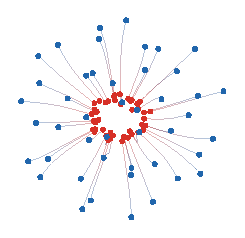
\includegraphics[width=.30\linewidth]{figures/gradflow-interaction-particles/repulsive.pdf} &
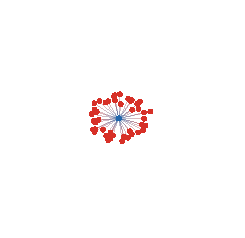
\includegraphics[width=.30\linewidth]{figures/gradflow-interaction-particles/attractive.pdf} &
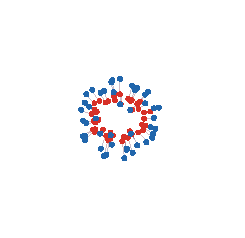
\includegraphics[width=.30\linewidth]{figures/gradflow-interaction-particles/attraction-repulsion.pdf}
\end{tabular}
\caption{\emph{Interaction-energy particle flows for three choices of $k$.} A positive Gaussian kernel $k(x,y)=\exp(-\norm{x-y}^2/(2\sigma^2))$ produces short-range repulsion under Wasserstein descent; changing its sign produces attraction and collapse; adding a quadratic long-range attraction to the repulsive kernel yields a balanced attraction--repulsion dynamics. The curves use arclength-based red-to-blue coloring along a longer integration of the coupled particle ODE~\eqref{eq:wassflows-particles}.}
\index{particle ODE}% strictindex
\index{energy!interaction}% strictindex
\label{fig:gradflow-interaction-particles}
\end{figure}

\begin{figure}[ht]
\centering
\begin{tabular}{@{}cccc@{}}
\small OT rays & \small MMD force & \small Sinkhorn force & \small drifting field \\[-.15em]

\includegraphics[width=.225\linewidth]{figures/gradflow-particle-objective-geometries/ot-rays.pdf} &
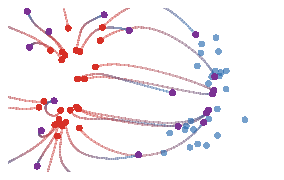
\includegraphics[width=.225\linewidth]{figures/gradflow-particle-objective-geometries/mmd-force.pdf} &
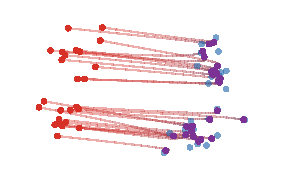
\includegraphics[width=.225\linewidth]{figures/gradflow-particle-objective-geometries/sinkhorn-divergence.pdf} &
\index{Sinkhorn divergence}% strictindex
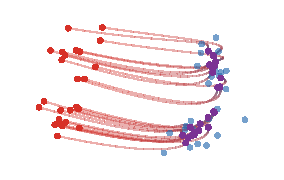
\includegraphics[width=.225\linewidth]{figures/gradflow-particle-objective-geometries/drifting-field.pdf}
\end{tabular}
\caption{\emph{Particle trajectories induced by different discrepancy geometries.} The red particles and blue target cloud are the same in all panels. Straight OT displacement produces rays from an optimal matching; an MMD-type witness field gives smoother nonlocal forces; the Sinkhorn-divergence force is an entropic, debiased transport attraction; and the normalized drifting field combines attraction to data with self-repulsion. The figure is qualitative: it compares geometric behavior, not solver performance.}
\label{fig:gradflow-particle-objective-geometries}
\end{figure}

\paragraph{Stochastic particles and McKean--Vlasov limits.}
\index{stochastic!particle}% strictindex
\index{McKean-Vlasov limit}% strictindex
\index{McKean-Vlasov equation}% strictindex
More generally, deterministic particle flows have stochastic counterparts, where Brownian noise at the particle level becomes an entropy term at the level of measures. If the drift does not depend on the empirical measure, each particle evolves independently according to
\index{empirical!measure}% strictindex
\[
	\d X_t=b(X_t)\d t+\sqrt{2}\sigma\d B_t,
\]
and the one-particle law $\alpha_t=\rho_t\d x$ directly satisfies the linear Fokker--Planck equation
\index{Fokker-Planck equation}% strictindex
\[
	\partial_t\rho_t=-\diverg(b\rho_t)+\sigma^2\Delta\rho_t.
\]

\begin{example}[Langevin drift as a free-energy flow]
	If $b=-\nabla V$, this linear Fokker--Planck equation is the $\Wass_2$ gradient flow of the free energy
	\[
		\rho\mapsto \int V\rho\,\d x+\sigma^2\int\rho\log\rho\,\d x.
	\]
\end{example}

The mean-field case is different: the drift is recomputed from the current empirical distribution of all particles,
\index{empirical!distribution}% strictindex
\index{gradient!flow}% strictindex
\index{mean-field limit}% strictindex
\[
	\d X_i^n(t)=b(X_i^n(t),\al_t^n)\d t+\sqrt{2}\sigma\d B_i(t),
	\qquad
	\al_t^n=\frac1n\sum_{i=1}^n\delta_{X_i^n(t)} .
\]
For finite $n$, the empirical law $\al_t^n$ is itself random. Under suitable Lipschitz, growth and chaotic-initialization assumptions, propagation of chaos states that finitely many particles become asymptotically independent as $n\to\infty$, all with the same deterministic law $\rho_t\d x$; equivalently, the empirical measure $\al_t^n$ converges in probability to this law. The limiting density solves the nonlinear Fokker--Planck, or McKean--Vlasov, equation
\index{Fokker-Planck equation}% strictindex
\index{McKean-Vlasov limit}% strictindex
\index{propagation of chaos}% strictindex
\index{empirical!law}% strictindex
\index{McKean-Vlasov equation}% strictindex
\[
	\partial_t \rho_t
	=
	-\diverg\big(b(x,\rho_t)\rho_t\big)
	+
	\sigma^2\Delta\rho_t .
\]
When the interaction drift has variational form
\[
	b(x,\rho)=-\nabla \frac{\delta \mathcal E}{\delta \rho}(x),
\]
	this PDE is the Wasserstein gradient flow of the entropy-regularized energy
\index{Wasserstein gradient}% strictindex
\index{gradient!flow}% strictindex
\index{Wasserstein!gradient flow}% strictindex
	\[
		\mathcal E(\rho)+\sigma^2\int \rho\log\rho\,\d x .
	\]

\begin{figure}[ht]
\centering
\begin{tabular}{@{}c@{}}
\small independent Langevin particles \\[-.15em]
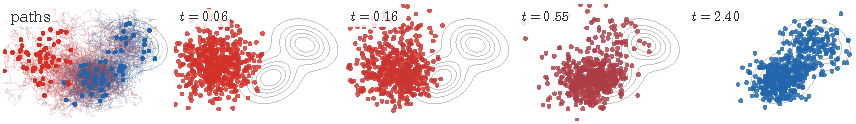
\includegraphics[width=.86\linewidth]{figures/gradflow-fokker-planck-three-representations/langevin-particles.pdf} \\[.25em]
\small deterministic KDE-score particles \\[-.15em]
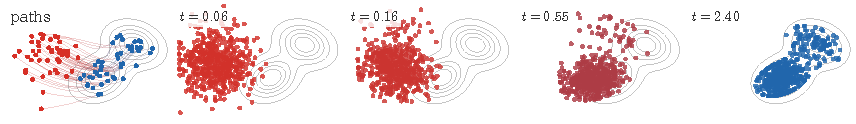
\includegraphics[width=.86\linewidth]{figures/gradflow-fokker-planck-three-representations/kde-particles.pdf} \\[.25em]
\small grid Fokker--Planck density \\[-.15em]
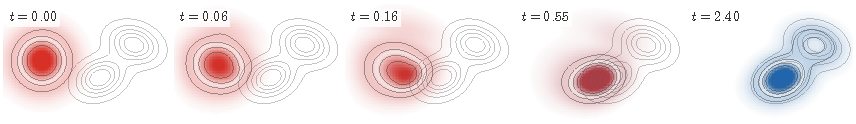
\includegraphics[width=.86\linewidth]{figures/gradflow-fokker-planck-three-representations/grid-pde.pdf}
\end{tabular}
\caption{\emph{Three numerical representations of an entropy-regularized Wasserstein gradient flow.} The target $\beta$ is a two-Gaussian density shifted to the right of an initially isotropic Gaussian density. The first row simulates independent Langevin particles and displays a thinned set of trajectories in the left panel. The second row evolves many deterministic particles with velocity $\tau(\nabla\log\rho_\beta-\nabla\log\rho_t)$, estimating $\nabla\log\rho_t$ by a sharper kernel-density score; only representative trajectories and particle subsets are displayed. The third row solves the corresponding Fokker--Planck equation on a grid, starting from the initial density in the left panel. The remaining columns use front-loaded times, so that the onset of the flow and the later deformation toward a bimodal law are both visible.}
\index{Wasserstein!gradient flow}% strictindex
\index{Fokker-Planck equation}% strictindex
\index{Langevin dynamics}% strictindex
\label{fig:gradflow-fokker-planck-three-representations}
\end{figure}


%%%
\paragraph{Gradient flows under density constraints.}
\index{density constraint}% strictindex
\index{crowd motion}% strictindex
\index{congestion}% strictindex

The same minimizing-movement formalism also handles nonsmooth energies. A prototypical example is a linear energy, generated by a potential, with a hard upper bound on the density,
\begin{equation}\label{eq-density-constrained-energy}
	F(\rho\d x)=\int_\Omega h(x)\rho(x)\d x+
	\iota_{\mathcal K_\kappa}(\rho\d x),
	\qquad
	\mathcal K_\kappa=
	\enscond{\rho\d x\in\Pp_2(\Omega)}{0\leq\rho\leq\kappa\ \text{a.e.}},
\end{equation}
where $\Omega\subset\RR^d$ is a convex domain and $\mathcal K_\kappa$ is assumed nonempty; if $\Omega$ has finite volume, this requires $\kappa|\Omega|\geq1$. The indicator term has no classical first variation; it contributes the normal cone to $\mathcal K_\kappa$ in the Wasserstein first-order condition. The JKO step becomes
\begin{equation}\label{eq-density-constrained-jko}
	\alpha^{k+1}
	\in
	\uargmin{\alpha\in\mathcal K_\kappa}
	\frac{1}{2\tau}\Wass_2^2(\alpha^k,\alpha)+\int_\Omega h\,\d\alpha .
\end{equation}
This is the mathematical mechanism behind macroscopic crowd-motion models with congestion, where the desired velocity $-\nabla h$ is projected onto velocities that do not increase density beyond the maximal value $\kappa$~\cite{maury2010macroscopic,SantambrogioCrowdReview}.
\index{normal cone}% strictindex
\index{maximal density constraint}% strictindex
\index{congestion}% strictindex

The hard cap is not especially benign numerically: the projection in the JKO step and the pressure field below can be difficult to compute accurately. Its advantage is geometric. Proposition~\ref{prop-density-cap-geodesic-convex} in Section~\ref{sec-geodesic-convexity} shows that $\mathcal K_\kappa$ is geodesically convex, so the indicator of the constraint is harmless for the usual geodesic-convex convergence guarantees.

The formal PDE contains a pressure field $p_t$, the Lagrange multiplier of the constraint. With no-flux boundary condition $\rho_t\nabla(h+p_t)\cdot n=0$ on $\partial\Omega$, the constrained gradient flow is the complementarity system
\index{pressure field}% strictindex
\begin{equation}\label{eq-density-constrained-pressure-flow}
	\partial_t\rho_t=\diverg\left(\rho_t\nabla(h+p_t)\right),
	\qquad
	0\leq\rho_t\leq\kappa,
	\qquad
	p_t\geq0,
	\qquad
	p_t(\kappa-\rho_t)=0.
\end{equation}
The pressure vanishes in the unsaturated region and acts only where $\rho_t=\kappa$, pushing mass away from congested zones so that the density cap remains satisfied.
\index{pressure field}% strictindex
\index{Lagrange multiplier}% strictindex

\begin{figure}[H]
\centering
\begin{tabular}{@{}ccc@{}}
\small small cap, $\kappa=.32$ & \small medium cap, $\kappa=.72$ & \small no cap, $\kappa=+\infty$ \\[-.15em]
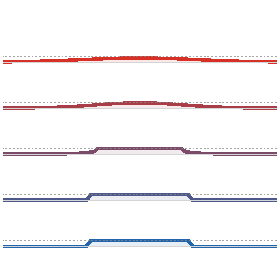
\includegraphics[width=.30\linewidth]{figures/gradflow-density-constrained-flow/kappa-small.pdf} &
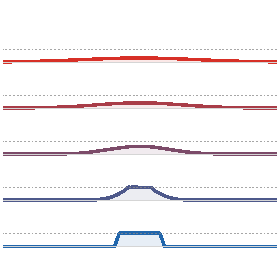
\includegraphics[width=.30\linewidth]{figures/gradflow-density-constrained-flow/kappa-medium.pdf} &
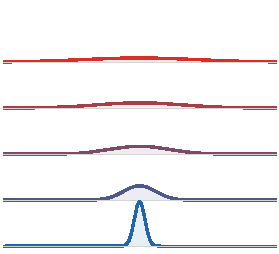
\includegraphics[width=.30\linewidth]{figures/gradflow-density-constrained-flow/unconstrained.pdf}
\end{tabular}
\caption{\emph{Density-constrained gradient flow under a quadratic attraction.} The one-dimensional flow is computed in quantile variables by explicit Lagrangian descent followed by the isotonic projection enforcing $\partial_s q\geq1/\kappa$. Each panel stacks five times vertically, colored from red to blue, using the same vertical density scale in all three panels. The dashed gray line marks the maximal density $\kappa$ for the constrained runs. A small cap forces the mass to form a wide saturated block, a medium cap allows a narrower congested region, and the unconstrained flow concentrates freely near the minimizer of $h$.}
\index{density constraint}% strictindex
\index{crowd motion}% strictindex
\index{pressure field}% strictindex
\label{fig:gradflow-density-constrained-flow}
\end{figure}

%%%
\paragraph{Multi-species gradient flows.}
\index{multi-species gradient flow}% strictindex
\index{vector-valued measure}% strictindex
\index{multi-species flow}% strictindex

Several applications involve several densities living on the same physical space: chemical species, color channels, cell populations or competing phases. Let $\Omega\subset\RR^d$ be the physical domain and assume that the component masses $\mathbf m=(m_1,\ldots,m_p)$ are positive and fixed. A convenient notation is
\begin{equation}\label{eq-multispecies-space}
	\Pp_{2,\mathbf m}(\Omega;\RR_+^p)=
	\enscond{\alpha=(\alpha_1,\ldots,\alpha_p)}
	{\alpha_i\in\Mm_+(\Omega),\ \alpha_i(\Omega)=m_i,\ \int_\Omega\norm{x}^2\d\alpha_i(x)<+\infty}.
\end{equation}
Since the components are finite measures rather than necessarily probabilities, set
\begin{equation}\label{eq-multispecies-product-metric}
	\Wass_{2,\oplus}^2(\alpha,\eta)=
	\sum_{i=1}^p m_i\,
	\Wass_2^2\!\left(\frac{\alpha_i}{m_i},\frac{\eta_i}{m_i}\right).
\end{equation}
This is the diagonal, independent-channel geometry; cross-effects may still enter through the energy or through constraints. In a more general vector-valued dynamic transport language, this is the special case of a diagonal mobility. The corresponding JKO step is
\begin{equation}\label{eq-multispecies-jko}
	\alpha^{k+1}
	\in
	\uargmin{\alpha\in\Pp_{2,\mathbf m}(\Omega;\RR_+^p)}
	\frac{1}{2\tau}\Wass_{2,\oplus}^2(\alpha^k,\alpha)+F(\alpha).
\end{equation}
For smooth densities and first variations $\phi_i=\delta F/\delta\rho_i$, this yields
\begin{equation}\label{eq-multispecies-pde}
	\partial_t\rho_i=\diverg\left(\rho_i\nabla\phi_i\right),
	\qquad
	\phi_i=\frac{\delta F}{\delta\rho_i},
	\qquad i=1,\ldots,p.
\end{equation}
The equations are independent only if $F$ is separable. Otherwise the coupling enters through the first variations $\phi_i$, not through the metric tensor. Carlier, Chizat and Laborde~\cite{CarlierChizatLabordeDisplacementSmoothness} use displacement smoothness of entropic OT to prove well-posedness of Wasserstein gradient flows that include multi-species systems. Congestion and shared-density variants are closely related to crowd and traffic models~\cite{maury2010macroscopic,CarlierSantambrogioOTCongestion2008,SantambrogioCrowdReview}.
\index{product Wasserstein metric}% strictindex
\index{JKO scheme}% strictindex

A second useful model imposes a pointwise composition constraint. Given a fixed reference density $\beta=b\d x$ with total mass $\sum_i m_i$, set
\begin{equation}\label{eq-multispecies-composition-constraint}
	\mathcal C_\beta=
	\enscond{\alpha\in\Pp_{2,\mathbf m}(\Omega;\RR_+^p)}
	{\sum_{i=1}^p \alpha_i=\beta}.
\end{equation}
The constrained JKO step is
\begin{equation}\label{eq-multispecies-constrained-jko}
	\alpha^{k+1}
	\in
	\uargmin{\alpha\in\mathcal C_\beta}
	\frac{1}{2\tau}\Wass_{2,\oplus}^2(\alpha^k,\alpha)+F(\alpha).
\end{equation}
In the smooth-density regime, the formal constrained flow has a common pressure $\lambda_t$:
\begin{equation}\label{eq-multispecies-constrained-pde}
	\partial_t\rho_i=\diverg\left(\rho_i\nabla(\phi_i-\lambda_t)\right),
	\qquad
	\diverg(b\nabla\lambda_t)=\diverg\left(\sum_{i=1}^p \rho_i\nabla\phi_i\right).
\end{equation}
For the separable Shannon entropy $F(\alpha)=\sum_i\int_\Omega \rho_i\log\rho_i\d x$, this becomes
\begin{equation}\label{eq-multispecies-modified-heat}
	\partial_t\rho_i=\Delta\rho_i-\diverg(\rho_i\nabla\lambda_t),
	\qquad
	\diverg(b\nabla\lambda_t)=\Delta b.
\end{equation}
When $b$ is constant, the pressure can be chosen constant and the system reduces to independent heat equations which nevertheless preserve the pointwise sum $\sum_i\rho_i=b$. This product geometry should be contrasted with vector-valued Benamou--Brenier distances, where the metric itself can couple the components through a non-diagonal mobility.
\index{Shannon entropy}% strictindex
\index{pressure field}% strictindex
\index{composition constraint}% strictindex

\begin{figure}[H]
\centering
\begin{tabular}{@{}ccc@{}}
\small $p=2$ species & \small $p=3$ species & \small $p=5$ species \\[-.15em]
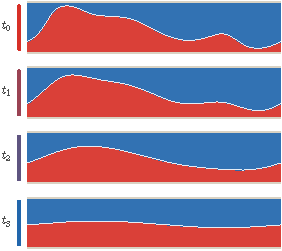
\includegraphics[width=.30\linewidth]{figures/gradflow-multispecies-entropy-flow/two-species.pdf} &
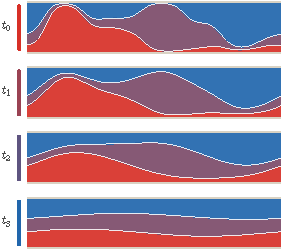
\includegraphics[width=.30\linewidth]{figures/gradflow-multispecies-entropy-flow/three-species.pdf} &
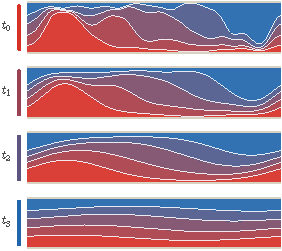
\includegraphics[width=.30\linewidth]{figures/gradflow-multispecies-entropy-flow/five-species.pdf}
\end{tabular}
\caption{\emph{Multi-species entropy flow under the shared-density constraint $\sum_i\rho_i=1$ on the periodic interval.} Each row is a time snapshot of the stacked densities, with the species shown as colored bands and time increasing from top to bottom. For a constant total density, the pressure in~\eqref{eq-multispecies-modified-heat} is constant, so each component follows the heat equation while the sum of the bands remains exactly flat.}
\index{multi-species gradient flow}% strictindex
\index{Shannon entropy}% strictindex
\index{density constraint}% strictindex
\label{fig:gradflow-multispecies-entropy-flow}
\end{figure}

\subsection{Geodesic Convexity and Convergence}
\index{convexity!geodesic}% strictindex
\label{sec-geodesic-convexity}

Geodesic convexity is the convexity notion adapted to Wasserstein geometry. It is the condition that turns the formal gradient-flow calculus into a convergence theory.
\index{gradient!flow}% strictindex
\index{geodesic convexity}% strictindex

\paragraph{Geodesics and convexity.}

A constant-speed $\Wass_2$ geodesic between $\alpha_0$ and $\alpha_1$ is obtained, as in Definition~\ref{def-w2-geodesic-induced-by-plan}, from any optimal coupling $\pi^\star\in\Couplings(\alpha_0,\alpha_1)$ by the McCann interpolation
\index{optimal coupling}% strictindex
\index{constant-speed geodesic}% strictindex
\index{McCann interpolation}% strictindex
\[
	\alpha_t=((1-t)P_0+tP_1)_\sharp\pi^\star,
	\qquad t\in[0,1],
\]
where $P_0(x,y)=x$ and $P_1(x,y)=y$. If the optimal plan is induced by a Brenier map $T$, this reduces to $((1-t)\Id+tT)_\sharp\alpha_0$. The coupling formula is important because geodesics exist even when no Monge map exists, for instance when a Dirac mass must split.
\index{Monge!problem}% strictindex
\index{optimal plan}% strictindex
\index{Brenier map}% strictindex
\index{Dirac mass}% strictindex

\begin{defn}[Geodesic convexity]\label{def-geodesic-convexity}
\index{convexity!geodesic}% strictindex
	A functional $f$ on $\Pp_2(\RR^d)$ is geodesically convex if for every $\Wass_2$ geodesic $(\alpha_t)_t$,
	\[
		f(\alpha_t)\leq (1-t)f(\alpha_0)+t f(\alpha_1).
	\]
	It is $\lambda$-geodesically convex if the right-hand side is improved by $-\frac{\lambda}{2}t(1-t)\Wass_2^2(\alpha_0,\alpha_1)$.
\end{defn}

\begin{prop}[Geodesic convexity of linear and quadratic energies]\label{prop-basic-geodesic-convexity}
\index{convexity!geodesic}% strictindex
	The following formal statements hold on $\Pp_2(\RR^d)$.
	\begin{enumerate}
		\item If $h$ is convex, then the linear energy $\alpha\mapsto\int h\d\alpha$ is geodesically convex; if $h$ is $\lambda$-strongly convex, it is $\lambda$-geodesically convex. Conversely, if this linear energy is geodesically convex for all Dirac endpoints, then $h$ is convex.
		\item More generally, let \(k\geq2\) and let \(H_k:(\RR^d)^k\to\RR\cup\{+\infty\}\) be convex. Then the polynomial energy
		\[
			\alpha\mapsto \int_{(\RR^d)^k} H_k(x_1,\ldots,x_k)\,\d\alpha(x_1)\cdots\d\alpha(x_k)
		\]
		is geodesically convex whenever the integral is well defined. In particular, the quadratic interaction
		\[
			\alpha\mapsto\frac12\iint W(x,y)\d\alpha(x)\d\alpha(y)
		\]
		is geodesically convex when \(W\) is convex on \(\RR^d\times\RR^d\).
\index{energy!interaction}% strictindex
	\end{enumerate}
\end{prop}
\begin{proof}
	Let \(\pi\) be an optimal coupling between \(\alpha_0\) and \(\alpha_1\), and set \(X_t=(1-t)X_0+tX_1\) under \((X_0,X_1)\sim\pi\). Convexity of \(h\) gives \(h(X_t)\leq(1-t)h(X_0)+t h(X_1)\), and strong convexity gives the additional term \(-\frac{\lambda}{2}t(1-t)\norm{X_0-X_1}^2\). Integrating proves the first claim. Necessity follows by testing on Dirac masses: the geodesic between \(\delta_x\) and \(\delta_y\) is \(\delta_{(1-t)x+ty}\), so geodesic convexity of \(\int h\d\alpha\) gives the usual convexity inequality for \(h\).

	For the polynomial statement, take \(k\) independent copies \((X_0^\ell,X_1^\ell)_{\ell=1}^k\) of the same optimal coupling and define \(X_t^\ell=(1-t)X_0^\ell+tX_1^\ell\). Convexity of \(H_k\) on the product space gives
	\[
		H_k(X_t^1,\ldots,X_t^k)
		\leq (1-t)H_k(X_0^1,\ldots,X_0^k)+tH_k(X_1^1,\ldots,X_1^k).
	\]
	Integrating over the product coupling proves the claim. The quadratic interaction is the special case \(k=2\).
\index{convexity!geodesic}% strictindex
\index{Monge!geodesic}% strictindex
\end{proof}

The polynomial criterion is useful but restrictive for kernel losses. MMD kernels are usually chosen for positive definiteness and statistical smoothing, not for convexity as functions of \((x,y)\). Gaussian and Laplace kernels, for instance, are not convex on \(\RR^d\times\RR^d\), so positive definiteness of \(k\) does not imply that \(\alpha\mapsto\MMD_k^2(\alpha,\beta)\) is geodesically convex. In fact, such MMD losses are not geodesically convex in general. One-dimensional monotone transport gives a sharper exception for distance-type kernels, because ordered quantiles keep the sign of pairwise differences fixed along geodesics; this is the one-dimensional displacement-convexity mechanism emphasized, for instance, in~\cite{SantambrogioBook}.
\index{maximum mean discrepancy}% strictindex
\index{kernel norm}% strictindex
\index{convexity!geodesic}% strictindex

\begin{prop}[One-dimensional interactions and energy-distance MMD]\label{prop-1d-interaction-halfline-convex}
\index{one-dimensional!transport}% strictindex
\index{convexity!geodesic}% strictindex
	Let \(\varphi:\RR_+\to\RR\) be continuous with at most quadratic growth, and define on \(\Pp_2(\RR)\)
	\[
		\mathcal I_\varphi(\alpha)
		\eqdef
		\frac12\iint \varphi(|x-y|)\d\alpha(x)\d\alpha(y).
	\]
	Then \(\mathcal I_\varphi\) is geodesically convex for \(\Wass_2\) on \(\Pp_2(\RR)\) if and only if \(\varphi\) is convex on \(\RR_+\).

	Fix also \(\beta\in\Pp_2(\RR)\). For the conditionally positive kernel \(k(x,y)=-|x-y|\), the squared MMD, equivalently the squared energy distance,
	\[
		\mathcal E_\beta(\alpha)
		\eqdef
		\MMD_k^2(\alpha,\beta)
		=
		\iint -|x-y|\,\d(\alpha-\beta)(x)\d(\alpha-\beta)(y),
	\]
	is geodesically convex as a function of \(\alpha\).
\end{prop}
\begin{proof}
	Let \(Q_0,Q_1\) be the quantile functions of \(\alpha_0,\alpha_1\), and let \(Q_t=(1-t)Q_0+tQ_1\) be the quantile function of the one-dimensional \(\Wass_2\) geodesic \(\alpha_t\). For \(r>s\), monotonicity gives \(Q_i(r)-Q_i(s)\geq0\) for \(i=0,1\), and hence
	\[
		Q_t(r)-Q_t(s)
		=
		(1-t)(Q_0(r)-Q_0(s))+t(Q_1(r)-Q_1(s)).
	\]
	Using the symmetry of the double integral and the quantile parametrization, one can write
	\[
		\mathcal I_\varphi(\alpha_t)
		=
		\int_0^1\int_0^r
		\varphi(Q_t(r)-Q_t(s))\,\d s\,\d r.
	\]
	Convexity of \(\varphi\) on \(\RR_+\) gives the desired convexity after integration.

	Conversely, test geodesic convexity on two-point measures \(\alpha_i=\frac12(\delta_0+\delta_{a_i})\), with \(a_i\geq0\). Their monotone geodesic is \(\alpha_t=\frac12(\delta_0+\delta_{(1-t)a_0+t a_1})\). Since
	\[
		\mathcal I_\varphi(\alpha_t)
		=
		\frac14\varphi(0)+\frac14\varphi((1-t)a_0+t a_1),
	\]
	and the identical \(\frac14\varphi(0)\) terms cancel from the geodesic-convexity inequality, one obtains the ordinary convexity inequality for \(\varphi\) on \(\RR_+\).

	For the energy distance, the function \(\varphi(r)=-r\) is affine on \(\RR_+\), so the self-interaction \(-\iint |x-y|\d\alpha(x)\d\alpha(y)\) is affine along one-dimensional Wasserstein geodesics even though \(z\mapsto-|z|\) is not convex on \(\RR\). Write \(Q_\beta\) for the quantile function of \(\beta\). Expanding the MMD and dropping the term depending only on \(\beta\) gives
	\[
		\mathcal E_\beta(\alpha)
		=
		2\int_0^1\!\!\int_0^1 |Q_\alpha(r)-Q_\beta(s)|\,\d r\,\d s
		-
		\int_0^1\!\!\int_0^1 |Q_\alpha(r)-Q_\alpha(s)|\,\d r\,\d s
		+\mathrm{constant}.
	\]
	Here the constant is independent of \(\alpha\). The positive cross-distance term is convex in \(Q_\alpha\), since the absolute value is convex and \(Q_t\) is affine in \(t\). The self-distance term is affine along quantile geodesics because
	\[
		\int_0^1\!\!\int_0^1 |Q_t(r)-Q_t(s)|\,\d r\,\d s
		=
		2\int_0^1\int_0^r (Q_t(r)-Q_t(s))\,\d s\,\d r.
	\]
	Thus \(\alpha\mapsto\mathcal E_\beta(\alpha)\) is geodesically convex.
\index{maximum mean discrepancy}% strictindex
\index{energy distance}% strictindex
\end{proof}

This one-dimensional result is the mechanism behind the favorable behavior of energy-distance particle flows discussed earlier in this chapter and in recent analyses of distance-kernel MMD flows~\cite{DuongRuxSteinSteidl2024DistanceMMD}. It should not be read as a general MMD statement: for a typical positive definite kernel \(k\), the decomposition
\[
	\MMD_k^2(\alpha,\beta)
	=
	\iint k\,\d\alpha\d\alpha
	-2\iint k\,\d\alpha\d\beta
	+\mathrm{constant}
\]
contains neither a convex self-interaction nor a convex cross term along Wasserstein geodesics.
\index{energy distance}% strictindex

Internal energies require a different mechanism: convexity is hidden in the Jacobian determinant of the transport map, not in a pointwise convex integrand along particles. The precise criterion is McCann's displacement-convexity theorem~\cite{mccann1997convexity}.

\begin{thm}[McCann displacement convexity for internal energies]\label{thm-mccann-internal-energy}
\index{McCann displacement convexity}% strictindex
\index{internal energy}% strictindex
\index{displacement convexity}% strictindex
	Let \(g:[0,+\infty)\to\RR\cup\{+\infty\}\) be convex with \(g(0)=0\), and define
	\[
		\psi(r)=r^d g(r^{-d}),\qquad r>0.
	\]
	If \(\psi\) is convex and nonincreasing on \((0,+\infty)\), then the internal energy
	\[
		\mathcal U_g(\alpha)=
		\begin{cases}
			\displaystyle \int_{\RR^d} g(\rho(x))\,\d x, & \alpha=\rho\d x,\\
			+\infty, & \text{otherwise},
		\end{cases}
	\]
	is geodesically convex on \(\Pp_2(\RR^d)\).
\end{thm}
\begin{proof}
	It is enough to prove the inequality for smooth positive compactly supported densities; the general case follows by approximation and lower semicontinuity. Let \(T=\nabla\varphi\) be the Brenier map from \(\alpha_0=\rho_0\d x\) to \(\alpha_1=\rho_1\d x\), set \(T_t=(1-t)\Id+tT\), and denote
	\[
		J_t(x)=\det\big((1-t)I+t\nabla T(x)\big).
	\]
	The interpolation satisfies \(\alpha_t=(T_t)_\sharp\alpha_0\) and
	\[
		\rho_t(T_t(x))J_t(x)=\rho_0(x).
	\]
	By concavity of \(\det^{1/d}\) on positive semidefinite matrices,
	\[
		J_t(x)^{1/d}\geq (1-t)+t\det(\nabla T(x))^{1/d}.
	\]
	Introduce \(s_t(x)=(J_t(x)/\rho_0(x))^{1/d}\). Since
	\(\rho_1(T(x))\det\nabla T(x)=\rho_0(x)\), this gives
	\[
		s_t(x)\geq (1-t)\rho_0(x)^{-1/d}+t\rho_1(T(x))^{-1/d}.
	\]
	Using the change of variables \(y=T_t(x)\), one obtains
	\[
		\int g(\rho_t(y))\,\d y
		=\int \rho_0(x)\,\psi(s_t(x))\,\d x .
	\]
	Because \(\psi\) is nonincreasing and convex,
	\[
		\psi(s_t(x))
		\leq (1-t)\psi(\rho_0(x)^{-1/d})+t\psi(\rho_1(T(x))^{-1/d}).
	\]
	Multiplying by \(\rho_0\) and integrating gives
	\(\mathcal U_g(\alpha_t)\leq(1-t)\mathcal U_g(\alpha_0)+t\mathcal U_g(\alpha_1)\).
\index{Jacobian determinant}% strictindex
\index{Brenier map}% strictindex
\end{proof}

The theorem applies to \(g(s)=s\log s\), since then \(\psi(r)=-d\log r\), to porous-medium powers \(g(s)=s^m/(m-1)\), \(m>1\), and more generally to the fast-diffusion range \(m\geq1-1/d\) when the energy is well defined, with \(m=1\) understood as the entropy limit.
The same criterion also clarifies which Csisz\'ar divergences inherit displacement convexity from an internal-energy structure.
\begin{prop}[Geodesic convexity of power divergences]\label{prop-power-divergences-geodesic-convexity}\label{prop-kl-gibbs-geodesic-convexity}
\index{relative entropy}% strictindex
\index{power divergence}% strictindex
\index{Csiszar divergence@Csisz\'ar divergence}% strictindex
\index{convexity!geodesic}% strictindex
	For \(m>0\), define
	\[
		\phi_m(r)=
		\begin{cases}
			\dfrac{r^m-mr+m-1}{m(m-1)}, & m\neq1,\\[2mm]
			r\log r-r+1, & m=1.
		\end{cases}
	\]
	Then the following geodesic-convexity statements hold.
	\begin{enumerate}
		\item If \(\Omega\subset\RR^d\) is convex, \(\beta=b\,\mathds{1}_\Omega\d x\), and \(m\geq1-1/d\), then \(\alpha\mapsto\Divergm_{\phi_m}(\alpha|\beta)\) is geodesically convex on \(\Pp_2(\Omega)\).
		\item If \(\beta=Z^{-1}e^{-V}\d x\) on \(\RR^d\), \(V\) is convex, and \(m\geq1\), then \(\alpha\mapsto\Divergm_{\phi_m}(\alpha|\beta)\) is geodesically convex on \((\Pp_2(\RR^d),\Wass_2)\).
		\item In the KL case \(m=1\), if \(V\) is \(\lambda\)-strongly convex, then \(\alpha\mapsto\KL(\alpha|\beta)=\Divergm_{\phi_1}(\alpha|\beta)\) is \(\lambda\)-geodesically convex.
	\end{enumerate}
	All statements use the convention that the divergence is \(+\infty\) when \(\alpha\) is not absolutely continuous with respect to \(\beta\).
\end{prop}
\begin{proof}
	For the flat reference case, write \(\alpha=\rho\d x\). Up to affine terms in \(\rho\), which only add constants on probability measures, the integrand \(b\,\phi_m(\rho/b)\) has non-affine part \(b^{1-m}\rho^m/(m(m-1))\) for \(m\neq1\), and \(\rho\log\rho\) for \(m=1\). For \(m=1\), McCann's criterion gives \(\psi(r)=-d\log r\). For \(m\neq1\), the transformed non-affine part is, up to the irrelevant factor \(b^{1-m}\),
	\[
		\psi_m(r)=\frac{r^{d(1-m)}}{m(m-1)}.
	\]
	If \(m>1\), this function is convex and nonincreasing. If \(0<m<1\), it is convex and nonincreasing exactly when \(d(1-m)\leq1\), i.e. \(m\geq1-1/d\). This proves the first claim by Theorem~\ref{thm-mccann-internal-energy}.

	Assume next that \(m>1\) and \(V\) is convex. Up to constants,
	\[
		\Divergm_{\phi_m}(\alpha|\beta)
		=
		\frac{Z^{m-1}}{m(m-1)}
		\int \rho(x)^m e^{(m-1)V(x)}\,\d x .
	\]
	Let \(T=\nabla\varphi\) be the Brenier map from \(\alpha_0=\rho_0\d x\) to \(\alpha_1\), set \(T_t=(1-t)\Id+tT\), and write
	\(J_t(x)=\det((1-t)I+t\nabla T(x))\). Along the geodesic \(\alpha_t=(T_t)_\sharp\alpha_0\),
	\[
		\int \rho_t^m e^{(m-1)V}\d x
		=
		\int \rho_0(x)^m
		\exp\!\left((m-1)\big(V(T_t(x))-\log J_t(x)\big)\right)\d x .
	\]
	For each \(x\), the function \(t\mapsto V(T_t(x))\) is convex, and \(t\mapsto-\log J_t(x)\) is convex because \(\log\det\) is concave on positive definite matrices. Since \(m-1>0\), the exponential of their sum is convex in \(t\). Integrating gives geodesic convexity. The nonsmooth case follows by approximation.

	Finally, for \(m=1\),
	\[
		\KL(\alpha|\beta)
		=
		\int \rho\log\rho\,\d x+\int V\d\alpha+\log Z.
	\]
	The entropy term is \(0\)-geodesically convex by Theorem~\ref{thm-mccann-internal-energy}. The linear potential term is \(\lambda\)-geodesically convex when \(V\) is \(\lambda\)-strongly convex, by Proposition~\ref{prop-basic-geodesic-convexity}. Taking \(\lambda=0\) also covers the \(m=1\) case in the second claim.
\end{proof}
\begin{rem}[Flat references and general \(\phi\)-divergences]\label{rem-phi-divergence-geodesic-convexity}
	The Csisz\'ar \(\phi\)-divergences behave like internal energies only in special reference geometries. If \(\beta=b\,\mathds{1}_{\Omega}\d x\) is proportional to Lebesgue measure on a bounded convex domain, then
	\[
		\Divergm_\phi(\alpha|\beta)
		=
		\int_{\Omega} b\,\phi(\rho(x)/b)\,\d x,
		\qquad \alpha=\rho\d x,
	\]
	so McCann's theorem applies whenever the integrand \(g(s)=b\,\phi(s/b)\) satisfies the displacement-convexity condition. For a nonuniform target \(\beta\), this reduction is no longer available. Proposition~\ref{prop-power-divergences-geodesic-convexity} gives a useful structured extension for the power family: log-concave targets preserve geodesic convexity for \(m\geq1\), while the KL endpoint is special in the stronger sense that \(\lambda\)-strong log-concavity gives \(\lambda\)-geodesic convexity. Outside such structured families, a generic \(\phi\)-divergence is not expected to be geodesically convex.

	The Hellinger integrand \(\phi_H(r)=(\sqrt r-1)^2\) illustrates why the qualifier ``flat reference'' matters. Since \(\phi_H=\phi_{1/2}/2\), Proposition~\ref{prop-power-divergences-geodesic-convexity} shows that the corresponding flat-reference internal energy is geodesically convex in dimension \(d=1\). The same \(\phi\)-divergence can nevertheless fail to be geodesically convex once the reference is nonuniform.

	A concrete Gaussian test shows the obstruction. Let \(\beta=\Gaussian(0,1)\) on \(\RR\) and \(\alpha_m=\Gaussian(m,1)\). The family \(m\mapsto\alpha_m\) is a \(\Wass_2\)-geodesic family, since the geodesic between \(\alpha_{m_0}\) and \(\alpha_{m_1}\) is \(\alpha_{(1-t)m_0+t m_1}\). Writing
	\[
		r_m(x)=\frac{\d\alpha_m}{\d\beta}(x)=\exp(mx-m^2/2),
	\]
	one obtains
	\[
		\Divergm_{\phi_H}(\alpha_m|\beta)
		=
		\int(\sqrt{r_m}-1)^2\,\d\beta
		=
		2\left(1-e^{-m^2/8}\right).
	\]
	Its second derivative is
	\[
		\frac{\d^2}{\d m^2}\Divergm_{\phi_H}(\alpha_m|\beta)
		=
		\frac12 e^{-m^2/8}\left(1-\frac{m^2}{4}\right),
	\]
	which is negative for \(|m|>2\). Thus the Hellinger \(\phi\)-divergence to a Gaussian target is not even \(0\)-geodesically convex. More generally, Gaussian translations reduce the question for any \(\phi\) to ordinary convexity of
	\[
		m\mapsto
		\EE_{X\sim\Gaussian(0,1)}
		\left[\phi\left(e^{mX-m^2/2}\right)\right],
	\]
	which need not hold. The KL integrand is special because this function is \(m^2/2\), up to the usual normalization.
\end{rem}
\index{Shannon entropy}% strictindex
\index{relative entropy}% strictindex

\paragraph{Geodesically convex constraints.}
\label{par-geodesically-convex-constraints}
\index{convexity!geodesic}% strictindex
\index{density constraint}% strictindex

Geodesic convexity is also useful for hard constraints. If a feasible set is geodesically convex, then adding its indicator to an energy does not destroy the variational structure used by minimizing movements and convergence arguments. The density cap from~\eqref{eq-density-constrained-energy} is the model example: it is numerically delicate, because one must compute a projection or a pressure, but it is geometrically compatible with Wasserstein descent.

\begin{proposition}[Geodesic convexity of density caps]\label{prop-density-cap-geodesic-convex}
\index{density constraint}% strictindex
\index{convexity!geodesic}% strictindex
	Assume that $\Omega\subset\RR^d$ is convex and let $\kappa>0$. The set $\mathcal K_\kappa$ in~\eqref{eq-density-constrained-energy} is geodesically convex in $\Pp_2(\Omega)$: if $\alpha_0,\alpha_1\in\mathcal K_\kappa$, then the constant-speed $\Wass_2$ geodesic $(\alpha_t)_{t\in[0,1]}$ between them also belongs to $\mathcal K_\kappa$.
\end{proposition}
\begin{proof}
	Assume first that the endpoints have smooth positive densities $\alpha_i=\rho_i\d x$ with $\rho_i\leq\kappa$, and let $T=\nabla\varphi$ be the Brenier map from $\alpha_0$ to $\alpha_1$. Since $\Omega$ is convex, $T_t=(1-t)\Id+tT$ maps $\Omega$ into $\Omega$. The interpolation is $\alpha_t=(T_t)_\sharp\alpha_0$ and
	\[
		\rho_t(T_t(x))=\frac{\rho_0(x)}{\det((1-t)I+t\nabla T(x))}.
	\]
	The concavity of $\det^{1/d}$ on positive semidefinite matrices and the identity $\rho_1(T(x))\det\nabla T(x)=\rho_0(x)$ give
	\[
		\rho_t(T_t(x))^{-1/d}
		\geq
		(1-t)\rho_0(x)^{-1/d}+t\rho_1(T(x))^{-1/d}
		\geq\kappa^{-1/d}.
	\]
	Hence $\rho_t\leq\kappa$ for all $t$. The general case follows by approximation and lower semicontinuity of the $L^\infty$ bound, as in McCann's displacement-convexity theory~\cite{mccann1997convexity}.
\index{Brenier map}% strictindex
\index{displacement interpolation}% strictindex
\end{proof}

\begin{example}[Squared Wasserstein distance need not be geodesically convex]
\index{convexity!geodesic}% strictindex
\index{non-convexity}% strictindex

The squared distance to a fixed measure is not geodesically convex in general. This is a sharp contrast with Hilbert spaces, where \(x\mapsto\norm{x-y}^2\) is convex along line segments. In \(\Pp_2(\RR^d)\), \(d\geq2\), take
\index{Wasserstein!squared distance}% strictindex
\index{Hilbert space}% strictindex
\[
	\beta=\frac12\de_{(-1/2,-1/2)}+\frac12\de_{(1/2,1/2)},
	\quad
	\alpha_0=\frac12\de_{(-1,0)}+\frac12\de_{(1,0)},
	\quad
	\alpha_1=\frac12\de_{(0,-1)}+\frac12\de_{(0,1)} .
\]
One optimal coupling between \(\alpha_0\) and \(\alpha_1\) matches \((-1,0)\) with \((0,1)\) and \((1,0)\) with \((0,-1)\). The associated geodesic has midpoint
\[
	\alpha_{1/2}=\frac12\de_{(-1/2,1/2)}+\frac12\de_{(1/2,-1/2)} .
\]
Then
\[
	\Wass_2^2(\alpha_0,\beta)
	=
	\Wass_2^2(\alpha_1,\beta)
	=
	\frac12,
	\qquad
	\Wass_2^2(\alpha_{1/2},\beta)
	=
	1,
\]
which violates geodesic convexity. Thus objectives built from squared Wasserstein distances can be non-convex in the Wasserstein geometry itself. This is one reason why optimal quantization, which minimizes \(\Wass_2^2(\alpha,\nu)\) over \(m\)-atomic measures \(\nu\), leads to non-convex algorithms such as Lloyd's method.
\index{Wasserstein!squared distance}% strictindex
\index{quantization!optimal}% strictindex
\index{Lloyd algorithm}% strictindex
\end{example}

\begin{rem}[Target discrepancies are usually semiconcave]\label{rem-target-discrepancies-semiconcave}
\index{geodesic semiconcavity}% strictindex
\index{generative model}% strictindex
	The preceding example is a useful warning. Losses of the form
	\(\alpha\mapsto D(\alpha,\beta)\), where \(\beta\) is a fixed target
	distribution, are rarely geodesically convex in the transport geometry. This is unfortunate for generative AI and generative modeling more broadly: training a distribution to match data by decreasing \(\Wass_2^2(\alpha,\beta)\), \(\SW_2^2(\alpha,\beta)\), or similar discrepancies should not be expected to inherit the convex behavior of Euclidean least squares.

	The squared Wasserstein loss has the opposite one-sided curvature: it is \(2\)-geodesically semiconcave along \(\Wass_2\) geodesics. More precisely, if \((\alpha_t)_{t\in[0,1]}\) is a constant-speed \(\Wass_2\) geodesic, then
	\[
		\Wass_2^2(\alpha_t,\beta)
		\geq
		(1-t)\Wass_2^2(\alpha_0,\beta)
		+
		t\Wass_2^2(\alpha_1,\beta)
		-
		t(1-t)\Wass_2^2(\alpha_0,\alpha_1).
	\]
	This is the standard \(2\)-geodesic semiconcavity convention for squared distances, often informally called ``\(2\)-concavity'': the graph may fall below the chord, but only by the quadratic correction \(t(1-t)\Wass_2^2(\alpha_0,\alpha_1)\). Equivalently, \(-\Wass_2^2(\cdot,\beta)\) is \((-2)\)-geodesically convex in the convention of Definition~\ref{def-geodesic-convexity}.

	To prove the estimate, write
	\(\alpha_t=((1-t)P_0+tP_1)_\sharp\pi_{01}\), where \(\pi_{01}\) is optimal between \(\alpha_0\) and \(\alpha_1\). Fix \(t\), put \(Z=(1-t)X_0+tX_1\), take an optimal coupling between \(\alpha_t\) and \(\beta\), and glue it with a disintegration of \(\pi_{01}\) over \(Z\). This gives random variables \((X_0,X_1,Y)\) such that \((Z,Y)\) is optimal between \(\alpha_t\) and \(\beta\), while \((X_0,X_1)\) is optimal between \(\alpha_0\) and \(\alpha_1\). Since \((X_i,Y)\) are admissible couplings between \(\alpha_i\) and \(\beta\),
	\[
		\Wass_2^2(\alpha_i,\beta)\leq \EE\norm{X_i-Y}^2,
		\qquad i=0,1.
	\]
	The Euclidean identity
	\[
		(1-t)\norm{X_0-Y}^2+t\norm{X_1-Y}^2
		=
		\norm{Z-Y}^2+t(1-t)\norm{X_0-X_1}^2
	\]
	then gives the claim after taking expectations.

	The sliced loss has the same flavor, but one must keep track of which geometry is used. The projection of a \(\Wass_2\) geodesic need not be the monotone one-dimensional geodesic between the projected endpoint measures. The preceding proof nevertheless applies after projection, using the projected coupling induced by \(\pi_{01}\). With the usual spherical normalization of sliced Wasserstein distances, this gives, along the same \(\Wass_2\) geodesic,
	\[
		\SW_2^2(\alpha_t,\beta)
		\geq
		(1-t)\SW_2^2(\alpha_0,\beta)
		+
		t\SW_2^2(\alpha_1,\beta)
		-
		\frac{t(1-t)}{d}\Wass_2^2(\alpha_0,\alpha_1),
	\]
	because the projection cost satisfies
	\(\int_{\Sphere^{d-1}}\abs{\dotp{\theta}{x_0-x_1}}^2\d\sigma(\theta)=\norm{x_0-x_1}^2/d\) and \(\pi_{01}\) is \(\Wass_2\)-optimal. Thus this is a semiconcavity estimate for the sliced discrepancy along \(\Wass_2\) geodesics, with a \(\Wass_2\)-controlled correction. If one instead works in the idealized Hilbert embedding by projected quantile functions, straight sliced chords satisfy the exact identity with the last term \(\SW_2^2(\alpha_0,\alpha_1)\). The caveat is that such straight chords need not be realized by actual measures on \(\RR^d\).
\end{rem}

\paragraph{Dissipation and finite metric length.}
\index{metric length bound}% strictindex
\index{Holder curve}% strictindex
\index{energy!dissipation}% strictindex
\index{energy-dissipation identity}% strictindex
\index{energy-dissipation inequality}% strictindex
\index{metric derivative}% strictindex
\index{finite metric length}% strictindex
\index{metric length}% strictindex
\index{gradient!flow}% strictindex

Before asking for convergence rates, one should first extract the basic information already contained in energy dissipation. For the classical gradient flow of a smooth function $h:\RR^d\to\RR$, $\dot x_t=-\nabla h(x_t)$, the chain rule gives
\[
	\frac{\d}{\d t}h(x_t)
	=
	-\norm{\nabla h(x_t)}^2
	=
	-\norm{\dot x_t}^2.
\]
Thus, for $0\leq s<t$, Cauchy's inequality gives
\begin{equation}\label{eq-euclidean-gradient-flow-length}
	\int_s^t \norm{\dot x_r}\,\d r
	\leq
	\sqrt{t-s}\left(\int_s^t\norm{\dot x_r}^2\d r\right)^{1/2}
	=
	\sqrt{t-s}\,\bigl(h(x_s)-h(x_t)\bigr)^{1/2}.
\end{equation}
The Wasserstein analogue uses the metric derivative $|\dot\alpha_t|_{\Wass_2}$ of an absolutely continuous curve. The following estimate isolates the only ingredient needed at this stage: energy dissipation controls the metric length of the path.

\begin{prop}[Finite metric length from dissipation]\label{prop-gradient-flow-finite-length}
\index{metric derivative}% strictindex
\index{energy!dissipation}% strictindex
\index{finite metric length}% strictindex
	Let $(\alpha_r)_{r\in[0,T]}$ be an absolutely continuous curve in $(\Pp_2(\RR^d),\Wass_2)$. Assume that, for all $0\leq s<t\leq T$, it satisfies the exact energy-dissipation identity
	\[
		f(\alpha_s)-f(\alpha_t)
		=
		\int_s^t |\dot\alpha_r|_{\Wass_2}^2\d r .
	\]
	Then
	\begin{equation}\label{eq-wasserstein-gradient-flow-length}
		\operatorname{Length}_{\Wass_2}\bigl((\alpha_r)_{r\in[s,t]}\bigr)
		=
		\int_s^t |\dot\alpha_r|_{\Wass_2}\,\d r
		\leq
		\sqrt{t-s}\,\bigl(f(\alpha_s)-f(\alpha_t)\bigr)^{1/2}.
	\end{equation}
	In the smooth Wasserstein gradient-flow setting with velocity $v_r=-\Wgrad f(\alpha_r)$, the dissipation identity reads equivalently
	\[
		f(\alpha_s)-f(\alpha_t)
		=
		\int_s^t |\dot\alpha_r|_{\Wass_2}^2\d r
		=
		\int_s^t\int \norm{v_r(x)}^2\d\alpha_r(x)\d r.
	\]
	If one assumes only the metric energy-dissipation inequality for a curve of maximal slope, then the same length estimate holds with the right-hand side multiplied by $\sqrt2$.
\end{prop}

\begin{proof}
	Cauchy's inequality gives
	\[
		\int_s^t |\dot\alpha_r|_{\Wass_2}\,\d r
		\leq
		\sqrt{t-s}
		\left(\int_s^t |\dot\alpha_r|_{\Wass_2}^2\d r\right)^{1/2}.
	\]
	The exact energy-dissipation identity substitutes the last integral by $f(\alpha_s)-f(\alpha_t)$, which proves~\eqref{eq-wasserstein-gradient-flow-length}. In the metric theory of curves of maximal slope~\cite{ambrosio2006gradient,SantambrogioBook}, the energy-dissipation inequality gives instead
	\[
		\frac12\int_s^t |\dot\alpha_r|_{\Wass_2}^2\d r
		\leq
		f(\alpha_s)-f(\alpha_t),
	\]
	and the same argument yields the additional factor $\sqrt2$.
\end{proof}

Proposition~\ref{prop-gradient-flow-finite-length} is weaker than a convergence rate: it does not identify a minimizer and it gives no decay law. It does, however, rule out escape to infinity in finite metric time whenever the energy is bounded below on finite time intervals. Indeed the trajectory segment remains in the \(\Wass_2\)-ball centered at \(\alpha_s\) with radius given by~\eqref{eq-wasserstein-gradient-flow-length}. It also gives a concrete modulus of continuity. If \(m_T\leq f(\alpha_r)\) for \(0\leq r\leq T\), then for \(0\leq s<t\leq T\),
\[
	\Wass_2(\alpha_s,\alpha_t)
	\leq
	\operatorname{Length}_{\Wass_2}\bigl((\alpha_r)_{r\in[s,t]}\bigr)
	\leq
	\sqrt{f(\alpha_0)-m_T}\,\sqrt{t-s},
\]
with an additional factor \(\sqrt2\) under the energy-dissipation inequality. Thus an energy-dissipating trajectory is \(1/2\)-H\"older continuous as a curve in Wasserstein space on every time interval where the energy remains bounded from below. Non-coercivity of the objective means that sublevel sets need not be compact, but an energy-dissipating curve still cannot travel an infinite \(\Wass_2\)-distance in finite time without an infinite energy drop. The convex estimate below adds a first quantitative conclusion under geodesic convexity; the PL viewpoint then gives sharper coercive rates toward minimizers.

\begin{prop}[Energy decay for convex Wasserstein flows]\label{prop-convex-wass-flow-rate}
\index{energy!decay}% strictindex
\index{Wasserstein!flow}% strictindex
	Assume formally that \(f\) is geodesically convex, admits a smooth first variation, and has a minimizer \(\alpha^\star\). Let \((\alpha_t)_t\) be a smooth solution of the Wasserstein gradient flow
\index{first variation}% strictindex
\index{Wasserstein gradient}% strictindex
\index{gradient!flow}% strictindex
\index{Wasserstein!gradient flow}% strictindex
	\[
		\partial_t\alpha_t+\diverg(\alpha_t v_t)=0,
		\qquad
		v_t=-\Wgrad f(\alpha_t).
	\]
	Then
	\[
		\frac{\d}{\d t} f(\alpha_t)
		=
		-\int \norm{\Wgrad f(\alpha_t)(x)}^2\,\d\alpha_t(x)
		\leq 0.
	\]
	If \(T_t\) is the optimal map from \(\alpha_t\) to \(\alpha^\star\), then
	\[
		f(\alpha_t)-f(\alpha^\star)
		\leq
		-\frac{\d}{\d t}\frac12 \Wass_2^2(\alpha_t,\alpha^\star),
	\]
	and consequently
	\[
		f(\alpha_t)-f(\alpha^\star)
		\leq
		\frac{\Wass_2^2(\alpha_0,\alpha^\star)}{2t}.
	\]
\end{prop}

\begin{proof}
	The chain rule and Proposition~\ref{prop-formal-wass-gradient} give
	\[
		\frac{\d}{\d t}f(\alpha_t)
		=
		\int \dotp{\Wgrad f(\alpha_t)(x)}{v_t(x)}\,\d\alpha_t(x)
		=
		-\int \norm{\Wgrad f(\alpha_t)(x)}^2\,\d\alpha_t(x).
	\]
	Geodesic convexity along the geodesic
\index{convexity!geodesic}% strictindex
\index{geodesic convexity}% strictindex
	\(((1-s)\Id+sT_t)_\sharp\alpha_t\) gives
	\[
		f(\alpha^\star)-f(\alpha_t)
		\geq
		\int \dotp{\Wgrad f(\alpha_t)(x)}{T_t(x)-x}\,\d\alpha_t(x).
	\]
	Since \(v_t=-\Wgrad f(\alpha_t)\), this reads
	\[
		f(\alpha_t)-f(\alpha^\star)
		\leq
		\int \dotp{v_t(x)}{T_t(x)-x}\,\d\alpha_t(x).
	\]
	The standard first-variation formula for the squared Wasserstein distance gives
\index{Wasserstein!distance}% strictindex
	\[
		\frac{\d}{\d t}\frac12\Wass_2^2(\alpha_t,\alpha^\star)
		=
		\int \dotp{x-T_t(x)}{v_t(x)}\,\d\alpha_t(x),
	\]
	which proves the differential inequality. Integrating it from \(0\) to \(t\) and using the monotonicity of \(s\mapsto f(\alpha_s)\) gives
	\[
		t\bigl(f(\alpha_t)-f(\alpha^\star)\bigr)
		\leq
		\int_0^t \bigl(f(\alpha_s)-f(\alpha^\star)\bigr)\,\d s
		\leq
		\frac12\Wass_2^2(\alpha_0,\alpha^\star).
	\]
\end{proof}


\paragraph{Convergence: the Wasserstein--PL viewpoint.}
\index{PL convergence}% strictindex
\index{metric slope}% strictindex
\index{Wasserstein-PL inequality}% strictindex
\index{Polyak-Lojasiewicz inequality}% strictindex

In general, analyzing \eqref{eq:wassflow-pde} is delicate. Geodesic convexity gives the familiar convex-gradient-flow picture, but rates are driven more directly by a first-order coercivity inequality. The relevant quantity is the squared Wasserstein slope
\[
	|\partial f|^2(\alpha)
	\eqdef
	\int\norm{\Wgrad f(\alpha)(x)}^2\,\d\alpha(x)
\]
in the smooth formal setting. Along a smooth gradient flow, this is both the squared metric speed and the energy-dissipation term.
\index{slope!Wasserstein}% strictindex
\index{energy!dissipation}% strictindex
\index{Kurdyka-Lojasiewicz inequality}% strictindex
\index{gradient inequality}% strictindex
The terminology mirrors the finite-dimensional Polyak--{\L}ojasiewicz condition introduced by Polyak~\cite{Polyak1963GradientMethods} and now standard in nonconvex optimization~\cite{KarimiNutiniSchmidt2016PL}. It is also part of the broader family of {\L}ojasiewicz and Kurdyka--{\L}ojasiewicz gradient inequalities used to prove convergence of dissipative dynamics~\cite{attouch-2010,HauerMazon2019KLSMetric,DelloSchiavoMaasPedrotti2023LocalConditions}. The Wasserstein version simply replaces the Euclidean gradient norm by the metric slope associated with \(\Wass_2\).

\begin{defn}[Wasserstein--Polyak--{\L}ojasiewicz inequality]\label{def-wasserstein-pl}
\index{Wasserstein-PL inequality}% strictindex
\index{Polyak-Lojasiewicz inequality}% strictindex
	Let \(f_\star\eqdef\inf_{\alpha\in\Pp_2(\RR^d)} f(\alpha)>-\infty\). The functional \(f\) satisfies the Wasserstein--PL inequality with constant \(\kappa>0\) if
	\begin{equation}\label{eq-wasserstein-pl}
		|\partial f|^2(\alpha)
		\geq
		2\kappa\bigl(f(\alpha)-f_\star\bigr)
	\end{equation}
	for every \(\alpha\) in the domain of \(f\). In the smooth Otto notation this reads
	\[
		\int\norm{\Wgrad f(\alpha)}^2\,\d\alpha
		\geq
		2\kappa\bigl(f(\alpha)-f_\star\bigr).
	\]
\end{defn}

\begin{thm}[Wasserstein--PL convergence]\label{thm-wasserstein-pl-convergence}
\index{Wasserstein-PL inequality}% strictindex
\index{linear!convergence}% strictindex
\index{energy!dissipation}% strictindex
	Assume that \(f_\star>-\infty\), that \(f\) satisfies the Wasserstein--PL inequality~\eqref{eq-wasserstein-pl} with constant \(\kappa>0\), and that \((\alpha_t)_{t\geq0}\) is a global Wasserstein gradient flow satisfying the full energy-dissipation identity
	\begin{equation}\label{eq-full-wasserstein-energy-dissipation}
		\frac{\d}{\d t}f(\alpha_t)
		=
		-|\dot\alpha_t|^2
		=
		-|\partial f|^2(\alpha_t)
		\qquad\text{for a.e. }t>0 .
	\end{equation}
	Set \(E(t)\eqdef f(\alpha_t)-f_\star\). Then, for \(0\leq s\leq t\),
	\[
		E(t)\leq e^{-2\kappa(t-s)}E(s),
	\]
	and the length of the flow segment satisfies
	\[
		\operatorname{Length}_{\Wass_2}\bigl((\alpha_r)_{r\in[s,t]}\bigr)
		\leq
		\sqrt{\frac{2}{\kappa}}\bigl(\sqrt{E(s)}-\sqrt{E(t)}\bigr).
	\]
	If, in addition, \(f\) is lower semicontinuous for \(\Wass_2\)-convergence, then \(\alpha_t\) converges in \(\Wass_2\) to a minimizer \(\alpha_\infty\in\operatorname{Argmin} f\), and
	\[
		\Wass_2(\alpha_t,\alpha_\infty)
		\leq
		\sqrt{\frac{2}{\kappa}}\sqrt{E(t)}
		\leq
		\sqrt{\frac{2}{\kappa}}\sqrt{E(0)}\,e^{-\kappa t}.
	\]
	In particular,
	\[
		\operatorname{dist}_{\Wass_2}(\alpha_t,\operatorname{Argmin}f)
		\leq
		\sqrt{\frac{2}{\kappa}}\sqrt{E(0)}\,e^{-\kappa t}.
	\]
\end{thm}

\begin{proof}
	The energy estimate is immediate from~\eqref{eq-full-wasserstein-energy-dissipation} and~\eqref{eq-wasserstein-pl}:
	\[
		E'(t)
		=
		-|\partial f|^2(\alpha_t)
		\leq
		-2\kappa E(t)
	\]
	for almost every \(t\). Gronwall's lemma gives \(E(t)\leq e^{-2\kappa(t-s)}E(s)\).

	The distance estimate uses the same two identities in a slightly different way. On the set where \(E(r)>0\), the PL inequality gives
	\[
		|\partial f|(\alpha_r)\geq \sqrt{2\kappa E(r)}.
	\]
	Using the full dissipation identity and \(|\dot\alpha_r|=|\partial f|(\alpha_r)\),
	\[
		\begin{aligned}
		\operatorname{Length}_{\Wass_2}\bigl((\alpha_r)_{r\in[s,t]}\bigr)
		&=
		\int_s^t|\dot\alpha_r|\,\d r
		=
		\int_s^t|\partial f|(\alpha_r)\,\d r \\
		&=
		\int_s^t
		\frac{|\partial f|^2(\alpha_r)}{|\partial f|(\alpha_r)}\,\d r
		\leq
		\frac{1}{\sqrt{2\kappa}}
		\int_s^t
		\frac{|\partial f|^2(\alpha_r)}{\sqrt{E(r)}}\,\d r \\
		&=
		\frac{1}{\sqrt{2\kappa}}
		\int_s^t
		\frac{-E'(r)}{\sqrt{E(r)}}\,\d r
		=
		\sqrt{\frac{2}{\kappa}}\bigl(\sqrt{E(s)}-\sqrt{E(t)}\bigr).
		\end{aligned}
	\]
	If \(E\) vanishes on a subinterval, then the flow is stationary there by~\eqref{eq-full-wasserstein-energy-dissipation}, so the same estimate follows by applying the argument on the part where \(E>0\). Since Wasserstein distance is bounded by metric length, the same upper bound controls \(\Wass_2(\alpha_s,\alpha_t)\).

	Letting \(t\to+\infty\), the energy estimate gives \(E(t)\to0\), and the length estimate shows that the tail of \((\alpha_t)_t\) is Cauchy. Since \((\Pp_2(\RR^d),\Wass_2)\) is complete, there is a limit \(\alpha_\infty\). Lower semicontinuity yields
	\[
		f(\alpha_\infty)
		\leq
		\liminf_{t\to+\infty}f(\alpha_t)
		=
		f_\star,
	\]
	hence \(\alpha_\infty\in\operatorname{Argmin}f\). Sending the endpoint of the length estimate to \(+\infty\) with \(s=t\) fixed gives
	\[
		\Wass_2(\alpha_t,\alpha_\infty)
		\leq
		\sqrt{\frac{2}{\kappa}}\sqrt{E(t)}.
	\]
	Combining this with the exponential energy decay gives the stated distance rate. The distance-to-the-set bound follows because \(\alpha_\infty\) is one minimizer.
\end{proof}

The exponential decay of the energy gap is the direct metric-gradient-flow analogue of the classical PL argument. The tail-length estimate used in Theorem~\ref{thm-wasserstein-pl-convergence} is a convenient way to turn this energy decay into a \(\Wass_2\)-distance-to-\(\operatorname{Argmin}f\) bound; this exact formulation was communicated to us by Rapha{\"e}l Barboni. More refined accounts of KL/PL-type inequalities, global convergence and rates for gradient flows and proximal point sequences in general metric spaces are given by Hauer and Maz{\'o}n~\cite{HauerMazon2019KLSMetric} and by Dello Schiavo, Maas and Pedrotti~\cite{DelloSchiavoMaasPedrotti2023LocalConditions}.

\paragraph{Geodesic strong convexity.}
Strong geodesic convexity is the cleanest geometric assumption behind the Wasserstein--PL inequality: it turns displacement convexity into a quantitative lower bound on the metric slope, so that the abstract convergence theorem above applies automatically.

\begin{prop}[Strong geodesic convexity implies Wasserstein--PL]\label{prop-strong-geodesic-convexity-implies-pl}
\index{convexity!strong geodesic}% strictindex
\index{Wasserstein-PL inequality}% strictindex
	Assume that \(f\) is \(\lambda\)-geodesically convex with \(\lambda>0\), that \(f_\star\) is attained at some \(\alpha^\star\), and that the Wasserstein slope is finite at \(\alpha\). Then
	\[
		|\partial f|^2(\alpha)
		\geq
		2\lambda\bigl(f(\alpha)-f_\star\bigr).
	\]
	Thus positive Wasserstein strong convexity implies the Wasserstein--PL inequality with the same constant.
\end{prop}

\begin{proof}
	Fix \(\alpha\) and a minimizer \(\alpha^\star\). Set
	\[
		g=f(\alpha)-f_\star,\qquad
		r=\Wass_2(\alpha,\alpha^\star),\qquad
		a=|\partial f|(\alpha).
	\]
	If \(r=0\), then \(\alpha=\alpha^\star\) and there is nothing to prove. Otherwise let \((\alpha_s)_{s\in[0,1]}\) be a constant-speed geodesic from \(\alpha\) to \(\alpha^\star\). By \(\lambda\)-geodesic convexity,
	\[
		f(\alpha_s)
		\leq
		(1-s)f(\alpha)+s f_\star
		-\frac{\lambda}{2}s(1-s)r^2.
	\]
	Therefore
	\[
		f(\alpha)-f(\alpha_s)
		\geq
		s g+\frac{\lambda}{2}s(1-s)r^2.
	\]
	Dividing by \(\Wass_2(\alpha,\alpha_s)=sr\) and letting \(s\downarrow0\) in the definition of the descending metric slope yields
	\[
		a\geq \frac{g}{r}+\frac{\lambda}{2}r.
	\]
	Equivalently, \(g\leq ar-\lambda r^2/2\). Maximizing the right-hand side over \(r\geq0\) gives \(g\leq a^2/(2\lambda)\), which is the desired PL inequality.
\index{slope!Wasserstein}% strictindex
\end{proof}

Together, Proposition~\ref{prop-strong-geodesic-convexity-implies-pl} and Theorem~\ref{thm-wasserstein-pl-convergence} recover the exponential energy rate \(e^{-2\lambda t}\) for positively geodesically convex Wasserstein gradient flows, and also give the distance rate \(e^{-\lambda t}\) toward the minimizer selected by the flow. The PL formulation is useful because it separates the first-order energy-dissipation mechanism from the stronger curvature requirement of geodesic convexity.

\begin{rem}[Convergence rates for classical examples]\label{rem-classical-convexity-rates}
	The examples needed to apply this implication have already been isolated above. Proposition~\ref{prop-basic-geodesic-convexity} gives \(\lambda\)-geodesic convexity for linear energies generated by \(\lambda\)-strongly convex potentials, and for the polynomial and pairwise interaction energies covered there when the corresponding finite-dimensional integrand is strongly convex. Theorem~\ref{thm-mccann-internal-energy} gives displacement convexity of internal energies, including entropy-type examples, and Proposition~\ref{prop-kl-gibbs-geodesic-convexity} adds the important nonflat case \(\KL(\cdot|\beta)\) when \(\d\beta=Z^{-1}e^{-V}\d x\) and \(V\) is strongly convex. Whenever these criteria yield a positive convexity constant, Proposition~\ref{prop-strong-geodesic-convexity-implies-pl} turns it into a Wasserstein--PL inequality, and Theorem~\ref{thm-wasserstein-pl-convergence} gives the corresponding linear convergence rates.
\end{rem}
\index{convexity!geodesic}% strictindex
\index{Wasserstein-PL inequality}% strictindex
\index{relative entropy}% strictindex

\paragraph{Convexity and curvature.}

The same language is not restricted to subsets of $\RR^d$. If $(\X,\dist,\mathfrak m)$ is a geodesic metric-measure space, $\Wass_2$ geodesics can be defined by transporting each pair of endpoints along metric geodesics, or more intrinsically by dynamical optimal plans on path space, as discussed in Section~\ref{sec-kantorovich-plan-interpolation}. Given a reference measure $\mathfrak m$, the entropy relative to $\mathfrak m$ is
\index{metric-measure space}% strictindex
\index{geodesic!space}% strictindex
\index{relative entropy}% strictindex
\index{dynamical optimal plan}% strictindex
\[
	\mathrm{Ent}_{\mathfrak m}(\alpha)
	\eqdef
	\begin{cases}
		\displaystyle \int_\X \rho\log\rho\,\d\mathfrak m,
		& \text{if } \alpha=\rho\,\mathfrak m,\\
		+\infty,
		& \text{otherwise.}
	\end{cases}
\]
On a smooth Riemannian manifold $(M,g)$, the Ricci curvature tensor $\mathrm{Ric}_g$ is the trace of the Riemann curvature tensor; the lower bound $\mathrm{Ric}_g\geq\lambda g$ means that $\mathrm{Ric}_g(v,v)\geq\lambda |v|_g^2$ for every tangent vector $v$. The fundamental link between curvature and optimal transport is that this tensor lower bound is exactly encoded by geodesic convexity of entropy.
\index{Ricci curvature}% strictindex
\index{Riemannian manifold}% strictindex
\index{convexity!geodesic}% strictindex

\begin{thm}[Ricci curvature and entropy convexity]\label{thm-ricci-entropy-convexity}
\index{relative entropy}% strictindex
	Let $(M,g)$ be a smooth compact connected Riemannian manifold without boundary, and let $\mathfrak m=\mathrm{vol}_g$. For $\lambda\in\RR$, the lower Ricci bound $\mathrm{Ric}_g\geq\lambda g$ holds if and only if $\mathrm{Ent}_{\mathfrak m}$ is $\lambda$-geodesically convex on $(\Pp_2(M),\Wass_2)$.
\end{thm}

This equivalence was developed in the smooth Riemannian setting by Cordero-Erausquin, McCann and Schmuckenschl{\"a}ger and by von Renesse and Sturm~\cite{cordero2001riemannian,vonrenesse2005transport}; it is a central theme of the optimal-transport approach to curvature in Villani's monograph~\cite{Villani09}. Lott--Villani and Sturm then used the same entropy-convexity principle to define synthetic lower Ricci curvature bounds on metric-measure spaces~\cite{lott2009ricci,sturm2006geometry1,sturm2006geometry2}. Outside this convex, curvature-controlled regime, such as in the mean-field neural-network example below, the flow may still be informative but its convergence analysis requires problem-specific arguments.
\index{metric-measure space}% strictindex
\index{synthetic Ricci curvature}% strictindex
\index{mean-field neural network}% strictindex
\index{mean-field limit}% strictindex


\subsection{Functional Inequalities via Optimal Transport}
\index{functional inequality}% strictindex
\index{isoperimetric inequality}% strictindex
\index{transport inequality}% strictindex

Optimal transport is also a proof technique for sharp inequalities. The common mechanism is simple: push one density to another by a monotone or Brenier map, interpolate along the transport rays, and convert convexity of the determinant, entropy, or the cost into an integral inequality. In the gradient-flow viewpoint of Section~\ref{sec-geodesic-convexity}, the inequalities that compare an energy gap with the squared Wasserstein slope are exactly Wasserstein--PL inequalities, and therefore imply rates through Theorem~\ref{thm-wasserstein-pl-convergence}. This section records a few representative examples. To keep the presentation readable, the proofs are written in the smooth Euclidean setting; the usual regularization and approximation arguments give the standard Borel or Sobolev versions. The transport viewpoint is developed systematically in McCann's displacement convexity principle, the Riemannian interpolation inequalities of Cordero-Erausquin, McCann and Schmuckenschl\"ager, and Villani's account of concentration and functional inequalities~\cite{mccann1997convexity,cordero2001riemannian,Villani09}.
\index{Brenier map}% strictindex
\index{displacement convexity}% strictindex
\index{Wasserstein-PL inequality}% strictindex

\paragraph{Brunn--Minkowski and isoperimetry.}
\index{Brunn-Minkowski inequality}% strictindex
\index{isoperimetric inequality}% strictindex
The most geometric use of OT is to prove that transporting two uniform measures and looking at the interpolated support increases volume at least concavely. The perimeter inequality is then obtained by differentiating this volume estimate after adding a small ball.

\begin{prop}[Brunn--Minkowski and Euclidean isoperimetry]\label{prop-ot-brunn-minkowski-isoperimetric}
	Let $A,B\subset\RR^d$ be bounded Borel sets with positive Lebesgue measure. For $t\in[0,1]$, set
	\[
		(1-t)A+tB\eqdef\{(1-t)x+ty\;:\;x\in A,\ y\in B\}.
	\]
	Then
	\[
		\mathrm{Vol}((1-t)A+tB)^{1/d}
		\geq
		(1-t)\mathrm{Vol}(A)^{1/d}
		+
		t\,\mathrm{Vol}(B)^{1/d}.
	\]
	Consequently, if $A$ is smooth and bounded and $\omega_d=\mathrm{Vol}(B_1)$, then
	\[
		\mathrm{Per}(A)
		\geq
		d\,\omega_d^{1/d}\mathrm{Vol}(A)^{(d-1)/d}.
	\]
\end{prop}

\begin{proof}
	We first give the argument for regular sets, the general Borel case following by approximation from inside and outside. Let $\alpha$ and $\beta$ be the uniform probability measures on $A$ and $B$, and let $T=\nabla\phi$ be the Brenier map with $T_\sharp\alpha=\beta$. The interpolating map $T_t=(1-t)\Id+tT$ sends $\alpha$ to a measure $\alpha_t$ supported in $(1-t)A+tB$. At points where $T$ is differentiable,
	\[
		\det DT_t
		=
		\det((1-t)\Id+tDT).
	\]
	Since $DT$ is symmetric positive semidefinite and $\det^{1/d}$ is concave on the positive semidefinite cone,
	\[
		\det(DT_t)^{1/d}
		\geq
		(1-t)+t\det(DT)^{1/d}.
	\]
	The change-of-variables identity for the uniform measures gives $\det(DT)=\mathrm{Vol}(B)/\mathrm{Vol}(A)$ almost everywhere. Hence the density $\rho_t$ of $\alpha_t$ satisfies
	\[
		\rho_t^{-1/d}
		\geq
		(1-t)\mathrm{Vol}(A)^{1/d}
		+
		t\mathrm{Vol}(B)^{1/d}.
	\]
	This means that $\rho_t\leq c_t^{-d}$ on its support, where $c_t=(1-t)\mathrm{Vol}(A)^{1/d}+t\mathrm{Vol}(B)^{1/d}$. Since $\alpha_t$ has total mass one and is supported in $(1-t)A+tB$, this gives $\mathrm{Vol}((1-t)A+tB)\geq c_t^d$, which is the displayed Brunn--Minkowski inequality.
\index{Brunn-Minkowski inequality}% strictindex

	For isoperimetry, apply Brunn--Minkowski with $B=B_1$ and write $A+\epsilon B_1$ for the parallel set. Then
\index{isoperimetric inequality}% strictindex
	\[
		\mathrm{Vol}(A+\epsilon B_1)^{1/d}
		\geq
		\mathrm{Vol}(A)^{1/d}+\epsilon\omega_d^{1/d}.
	\]
	Using $\mathrm{Vol}(A+\epsilon B_1)=\mathrm{Vol}(A)+\epsilon\,\mathrm{Per}(A)+o(\epsilon)$ and differentiating at $\epsilon=0$ yields the claimed perimeter bound.
\end{proof}

Figure~\ref{fig:gradflow-brunn-minkowski-ot} isolates the determinant-concavity step in the special case where the optimal map is affine.

\begin{figure}
\centering
\setlength{\tabcolsep}{1.5pt}
\begin{tabular}{@{}cccccc@{}}

\includegraphics[width=.118\linewidth]{figures/gradflow-brunn-minkowski-ot/ellipse-t000.pdf} &

\includegraphics[width=.118\linewidth]{figures/gradflow-brunn-minkowski-ot/ellipse-t025.pdf} &

\includegraphics[width=.118\linewidth]{figures/gradflow-brunn-minkowski-ot/ellipse-t050.pdf} &

\includegraphics[width=.118\linewidth]{figures/gradflow-brunn-minkowski-ot/ellipse-t075.pdf} &

\includegraphics[width=.118\linewidth]{figures/gradflow-brunn-minkowski-ot/ellipse-t100.pdf} &

\includegraphics[width=.265\linewidth]{figures/gradflow-brunn-minkowski-ot/area-concavity.pdf} \\[-.1em]
\small $t=0$ & \small $t=.25$ & \small $t=.5$ & \small $t=.75$ & \small $t=1$ & \small area inequality
\end{tabular}
\caption{\emph{Brunn--Minkowski through an affine optimal-transport interpolation between two ellipses.} For ellipses, the Brenier map is affine, so the transported support $T_t(A)$ remains an ellipse and its area is computed exactly from the determinant of $(1-t)\Id+tDT$. The right panel shows that $|T_t(A)|^{1/2}$ lies above the linear interpolation of the endpoint square-root areas, which is the two-dimensional determinant concavity behind the proof of Brunn--Minkowski.}
\label{fig:gradflow-brunn-minkowski-ot}
\index{Brunn-Minkowski inequality}% strictindex
\index{Brenier map}% strictindex
\end{figure}

\paragraph{Pr\'ekopa--Leindler.}
\index{Prekopa-Leindler inequality}% strictindex
\index{functional inequality}% strictindex
The functional analogue of Brunn--Minkowski replaces sets by densities. The transport proof is the same argument with the Jacobian no longer constant.

\begin{prop}[Pr\'ekopa--Leindler inequality]\label{prop-ot-prekopa-leindler}
	Let $u,v,w:\RR^d\to[0,+\infty)$ be integrable, and let $t\in[0,1]$. Assume that
	\[
		w((1-t)x+ty)\geq u(x)^{1-t}v(y)^t
		\qquad
		\text{for all }x,y\in\RR^d.
	\]
	Then
	\[
		\int_{\RR^d} w
		\geq
		\left(\int_{\RR^d}u\right)^{1-t}
		\left(\int_{\RR^d}v\right)^t .
	\]
\end{prop}

\begin{proof}
	Set $U=\int u$ and $V=\int v$, and assume $U,V>0$. Let $\alpha=(u/U)\d x$ and $\beta=(v/V)\d x$, and let $T$ be the Brenier map from $\alpha$ to $\beta$. Put $T_t=(1-t)\Id+tT$. The change of variables gives
	\[
		\int w
		\geq
		\int w(T_t(x))\det(DT_t(x))\d x .
	\]
	By the assumption on $w$ and by $\det((1-t)\Id+tDT)\geq\det(DT)^t$ for positive semidefinite $DT$,
	\[
		\int w
		\geq
		\int u(x)^{1-t}v(T(x))^t\det(DT(x))^t\d x.
	\]
	Since $T_\sharp\alpha=\beta$, the Monge--Amp\`ere identity gives
	\[
		\det(DT(x))=\frac{u(x)V}{v(T(x))U}
	\]
	almost everywhere. Substitution yields
	\[
		\int w
		\geq
		\left(\frac{V}{U}\right)^t\int u(x)\d x
		=
		U^{1-t}V^t.
	\]
	Approximation removes the smoothness and positivity assumptions.
\end{proof}


\paragraph{Logarithmic Sobolev inequalities.}
\index{logarithmic Sobolev inequality}% strictindex
\index{Fisher information}% strictindex
The logarithmic Sobolev inequality is the slope-coercivity estimate that turns entropy into a quantitative relaxation principle. Let \(\beta=\rho_\beta\d x\) be a reference probability measure and let \(\alpha=h\beta\). The relative Fisher information is
\[
	\mathcal I_\beta(\alpha)
	\eqdef
	\int \norm{\nabla\log h}^2\,\d\alpha
	=
	\int \frac{\norm{\nabla h}^2}{h}\,\d\beta,
\]
with value \(+\infty\) when \(\alpha\) is not absolutely continuous with respect to \(\beta\), or when the expression is not finite. One says that \(\beta\) satisfies the logarithmic Sobolev inequality with constant \(\lambda>0\) if
\begin{equation}\label{eq-general-log-sobolev}
	\KL(\alpha|\beta)
	\leq
	\frac{1}{2\lambda}\mathcal I_\beta(\alpha)
	\qquad
	\text{for all probability measures }\alpha.
\end{equation}
This is not a universal statement about all reference measures; it is a regularity and confinement property of \(\beta\). A standard sufficient condition is positive curvature of the potential. We formulate it before the Gaussian example because it is the natural general form of the inequality; the proof uses the HWI estimate proved later in this section.

\begin{prop}[Curvature implies logarithmic Sobolev]\label{prop-curvature-log-sobolev}
\index{Bakry-Emery criterion}% strictindex
\index{log-concavity}% strictindex
	Let \(\beta=Z^{-1}e^{-V}\d x\) be a smooth probability measure on \(\RR^d\). If \(\nabla^2V\succeq\lambda\Id\) for some \(\lambda>0\), then \(\beta\) satisfies \eqref{eq-general-log-sobolev} with constant \(\lambda\).
\end{prop}

\begin{proof}
	Apply the HWI inequality of Proposition~\ref{prop-hwi-inequality}. Under the curvature assumption, for every absolutely continuous \(\alpha\),
	\[
		\KL(\alpha|\beta)
		\leq
		\Wass_2(\alpha,\beta)\sqrt{\mathcal I_\beta(\alpha)}
		-
		\frac{\lambda}{2}\Wass_2^2(\alpha,\beta).
	\]
	For fixed \(s=\sqrt{\mathcal I_\beta(\alpha)}\), maximize the right-hand side over \(r=\Wass_2(\alpha,\beta)\geq0\). The elementary inequality \(rs-\lambda r^2/2\leq s^2/(2\lambda)\) gives \eqref{eq-general-log-sobolev}. Approximation gives the usual nonsmooth statement. This is the Bakry--Emery mechanism expressed in the optimal-transport language; the direct \(\Gamma_2\) proof gives the same criterion.
\end{proof}

\begin{rem}[Logarithmic Sobolev as Wasserstein--PL]\label{rem-lsi-wasserstein-pl}
\index{Wasserstein-PL inequality}% strictindex
\index{relative Fisher information}% strictindex
	For \(F(\alpha)=\KL(\alpha|\beta)\), the Wasserstein gradient is
	\[
		\Wgrad F(\alpha)
		=
		\nabla\log\frac{\d\alpha}{\d\beta},
	\]
	and its squared Wasserstein slope is precisely the relative Fisher information,
	\[
		|\partial F|^2(\alpha)=\mathcal I_\beta(\alpha).
	\]
	Since the unique minimizer is \(\beta\) and \(F(\beta)=0\), \eqref{eq-general-log-sobolev} is exactly
	\[
		|\partial F|^2(\alpha)
		\geq
		2\lambda\bigl(F(\alpha)-F(\beta)\bigr),
	\]
	that is, the Wasserstein--PL inequality of Definition~\ref{def-wasserstein-pl}. Thus logarithmic Sobolev is the functional-inequality incarnation of the convergence mechanism studied in Section~\ref{sec-geodesic-convexity}, and Theorem~\ref{thm-wasserstein-pl-convergence} converts it into exponential decay of both entropy and Wasserstein distance to equilibrium.
\end{rem}

\begin{prop}[Logarithmic Sobolev inequality implies entropy decay]\label{prop-lsi-entropy-decay}
\index{Fokker-Planck equation}% strictindex
\index{entropy decay}% strictindex
	Let \(\beta=e^{-V}\d x/Z\) be a smooth probability measure on \(\RR^d\) satisfying the logarithmic Sobolev inequality \eqref{eq-general-log-sobolev} with constant \(\lambda>0\). Let \(\alpha_t\) solve the Wasserstein gradient flow of \(F(\alpha)=\KL(\alpha|\beta)\), namely
	\[
		\partial_t\rho_t
		=
		\nabla\cdot(\rho_t\nabla V)+\Delta\rho_t,
		\qquad
		\alpha_t=\rho_t\d x .
	\]
	If \(\KL(\alpha_0|\beta)<+\infty\), then
	\[
		\KL(\alpha_t|\beta)
		\leq
		e^{-2\lambda t}\KL(\alpha_0|\beta).
	\]
	Moreover, if \(\beta\in\Pp_2(\RR^d)\), then
	\[
		\Wass_2(\alpha_t,\beta)
		\leq
		\sqrt{\frac{2}{\lambda}\KL(\alpha_0|\beta)}\,e^{-\lambda t}.
	\]
\end{prop}

\begin{proof}
	The first variation of \(F\) is \(\log(\rho/\rho_\beta)\), up to an additive constant. Along the smooth Wasserstein gradient flow,
	\[
		\frac{\d}{\d t}\KL(\alpha_t|\beta)
		=
		-\int \norm{\nabla\log\frac{\d\alpha_t}{\d\beta}}^2\,\d\alpha_t
		=
		-\mathcal I_\beta(\alpha_t).
	\]
	The logarithmic Sobolev inequality bounds the Fisher information below by \(2\lambda\KL(\alpha_t|\beta)\). Hence
\index{logarithmic Sobolev inequality}% strictindex
	\[
		\frac{\d}{\d t}\KL(\alpha_t|\beta)
		\leq
		-2\lambda\KL(\alpha_t|\beta),
	\]
	and Gronwall's lemma gives the entropy estimate. The Wasserstein estimate follows from the length estimate in the Wasserstein--PL theorem: apply Theorem~\ref{thm-wasserstein-pl-convergence} to \(F=\KL(\cdot|\beta)\), whose unique minimizer is \(\beta\), and use Remark~\ref{rem-lsi-wasserstein-pl}.
\end{proof}

\paragraph{Gaussian logarithmic Sobolev inequality.}
\index{logarithmic Sobolev inequality}% strictindex
\index{Gaussian measure}% strictindex
The standard Gaussian is the model case where the optimal constant is known exactly. With the convention of \eqref{eq-general-log-sobolev}, \(\gamma_d=\mathcal N(0,\Id)\) satisfies the logarithmic Sobolev inequality with \(\lambda=1\), and this value is sharp. Transport gives a short proof of the inequality: the Jacobian equation for the Brenier map is bounded by \(\log\det A\leq\tr(A-\Id)\), and Gaussian integration by parts converts the trace term into Fisher information.

\begin{prop}[Gaussian logarithmic Sobolev inequality]\label{prop-gaussian-log-sobolev-ot}
\index{Fisher information}% strictindex
	Let \(\gamma_d\) be the standard Gaussian measure on \(\RR^d\). If \(\rho\) is smooth, positive, has sufficient decay, and \(\int \rho\d\gamma_d=1\), then
	\[
		\mathrm{Ent}_{\gamma_d}(\rho)
		\eqdef
		\int \rho\log \rho\,\d\gamma_d
		\leq
		\frac12\int \frac{\norm{\nabla \rho}^2}{\rho}\,\d\gamma_d.
	\]
\end{prop}

\begin{proof}
	Let \(\al=\rho\gamma_d\), and let \(T=\nabla\phi\) be the Brenier map with \(T_\sharp\al=\gamma_d\). Write \(T(x)=x+\theta(x)\). The Monge--Amp\`ere equation reads
	\[
		\rho(x)e^{-\norm{x}^2/2}
		=
		e^{-\norm{T(x)}^2/2}\det(DT(x)).
	\]
	Thus
	\[
		\log \rho(x)
		=
		-\dotp{x}{\theta(x)}
		-\frac12\norm{\theta(x)}^2
		+
		\log\det(\Id+D\theta(x)).
	\]
	Since \(DT\) is positive semidefinite, \(\log\det(\Id+D\theta)\leq\tr(D\theta)=\diverg\theta\). Multiplying by \(\rho\) and integrating with respect to \(\gamma_d\) gives
	\[
		\mathrm{Ent}_{\gamma_d}(\rho)
		\leq
		\int \rho(\diverg\theta-\dotp{x}{\theta})\,\d\gamma_d
		-\frac12\int \rho\norm{\theta}^2\,\d\gamma_d.
	\]
	Gaussian integration by parts gives
	\[
		\int \rho(\diverg\theta-\dotp{x}{\theta})\,\d\gamma_d
		=
		-\int\dotp{\nabla \rho}{\theta}\,\d\gamma_d.
	\]
	Completing the square pointwise,
	\[
		-\dotp{\nabla \rho}{\theta}-\frac12 \rho\norm{\theta}^2
		\leq
		\frac12\frac{\norm{\nabla \rho}^2}{\rho}.
	\]
	This proves the inequality. The general Sobolev-class statement follows by approximation.
\end{proof}

The constant cannot be improved. For a translation tilt
\[
	\rho_a(x)=\exp\!\left(\dotp{a}{x}-\frac12\norm{a}^2\right),
	\qquad a\in\RR^d,
\]
one has \(\rho_a\gamma_d=\mathcal N(a,\Id)\). A direct computation gives
\[
	\int \rho_a\log \rho_a\,\d\gamma_d
	=
	\frac12\norm{a}^2,
	\qquad
	\frac12\int\frac{\norm{\nabla \rho_a}^2}{\rho_a}\,\d\gamma_d
	=
	\frac12\norm{a}^2.
\]
Thus equality is attained along translations, and the sharp logarithmic Sobolev constant of the standard Gaussian is \(\lambda=1\). Proposition~\ref{prop-lsi-entropy-decay} then gives the classical exponential convergence of the Ornstein--Uhlenbeck flow.
\index{Ornstein-Uhlenbeck flow}% strictindex

\paragraph{Poincar\'e as a linearized Wasserstein--PL inequality.}
\index{Poincare inequality}% strictindex
\index{linearized Wasserstein metric}% strictindex
Functional inequalities often appear by zooming in on a nonlinear convergence inequality near an equilibrium. If an energy \(\Ff\) satisfies a Wasserstein--PL inequality and \(\beta\) is a minimizer, then perturbing \(\beta\) by a small density modulation turns the nonlinear PL bound into a quadratic inequality for the perturbation.

\begin{prop}[Linearizing a Wasserstein--PL inequality]\label{prop-linearized-pl-functional-inequality}
\index{Wasserstein-PL inequality}% strictindex
\index{functional inequality}% strictindex
	Let \(\beta\) be a minimizer of an energy \(\Ff\), and assume that \(\Ff\) satisfies the Wasserstein--PL inequality with constant \(\kappa>0\), namely \eqref{eq-wasserstein-pl} with \(f\) replaced by \(\Ff\). Let \(\varphi\) be a smooth bounded perturbation with \(\int\varphi\,\d\beta=0\), and set \(\alpha_\epsilon=(1+\epsilon\varphi)\beta\) for \(|\epsilon|\) small enough. Assume that, as \(\epsilon\to0\),
	\[
		\Ff(\alpha_\epsilon)-\Ff(\beta)
		=
		\frac{\epsilon^2}{2}\,\mathsf H_\beta(\varphi)+o(\epsilon^2),
		\qquad
		|\partial\Ff|^2(\alpha_\epsilon)
		=
		\epsilon^2\,\mathsf D_\beta(\varphi)+o(\epsilon^2).
	\]
	Then the perturbation satisfies the linearized functional inequality
	\[
		\kappa\,\mathsf H_\beta(\varphi)
		\leq
		\mathsf D_\beta(\varphi).
	\]
\end{prop}

\begin{proof}
	Applying the PL inequality to \(\alpha_\epsilon\) gives
	\[
		|\partial\Ff|^2(\alpha_\epsilon)
		\geq
		2\kappa\bigl(\Ff(\alpha_\epsilon)-\Ff(\beta)\bigr),
	\]
	because \(\Ff(\beta)\) is the minimum value. Substituting the two second-order expansions, dividing by \(\epsilon^2\), and letting \(\epsilon\to0\) gives the claim.
\end{proof}

The most striking instance is the entropy energy \(\Ff(\alpha)=\KL(\alpha|\beta)\). In this case the squared Wasserstein slope is the relative Fisher information, so the PL inequality is precisely the logarithmic Sobolev inequality. Its linearization is the Poincar\'e inequality.
\index{relative Fisher information}% strictindex
\index{logarithmic Sobolev inequality}% strictindex

\begin{prop}[Poincar\'e from logarithmic Sobolev]\label{prop-poincare-linearized-wasserstein-pl}
\index{Poincare inequality}% strictindex
\index{spectral gap}% strictindex
	Let \(\beta\) be a smooth probability measure on \(\RR^d\). Assume that \(\beta\) satisfies the logarithmic Sobolev inequality with constant \(\kappa>0\),
	\[
		\KL(\alpha|\beta)
		\leq
		\frac{1}{2\kappa}\,\mathcal I_\beta(\alpha),
		\qquad
		\mathcal I_\beta(\alpha)
		\eqdef
		\int\norm{\nabla\log\frac{\d\alpha}{\d\beta}}^2\,\d\alpha .
	\]
	Then, for every smooth \(\varphi\) with \(\int\varphi\,\d\beta=0\),
	\[
		\kappa\int\varphi^2\,\d\beta
		\leq
		\int\norm{\nabla\varphi}^2\,\d\beta .
	\]
	In particular, if \(\d\beta=Z^{-1}e^{-V}\d x\) and \(\nabla^2 V\succeq \kappa\Id\), so that \(\beta\) is \(\kappa\)-strongly log-concave, then the conclusion holds by the Bakry--Emery criterion.
\end{prop}

\begin{proof}
	For \(h_\epsilon=1+\epsilon\varphi\), with \(|\epsilon|\) small enough, one has \(\alpha_\epsilon=h_\epsilon\beta\) and
	\[
		\KL(\alpha_\epsilon|\beta)
		=
		\int h_\epsilon\log h_\epsilon\,\d\beta
		=
		\frac{\epsilon^2}{2}\int\varphi^2\,\d\beta+o(\epsilon^2),
	\]
	because \(\int\varphi\,\d\beta=0\). The Fisher information expands as
	\[
		\mathcal I_\beta(\alpha_\epsilon)
		=
		\int\norm{\nabla\log h_\epsilon}^2 h_\epsilon\,\d\beta
		=
		\epsilon^2\int\norm{\nabla\varphi}^2\,\d\beta+o(\epsilon^2).
	\]
	Inserting these expansions in the logarithmic Sobolev inequality and letting \(\epsilon\to0\) gives the Poincar\'e inequality. The last assertion is the usual Bakry--Emery implication from \(\kappa\)-convexity of \(V\) to the logarithmic Sobolev inequality.
\end{proof}

If \(\d\beta=\rho_\beta\d x=Z^{-1}e^{-V}\d x\), the Poincar\'e inequality is equivalently a spectral gap for the \(\beta\)-weighted Laplacian
\[
	L_\beta\varphi
	\eqdef
	\Delta\varphi-\dotp{\nabla V}{\nabla\varphi}
	=
	\rho_\beta^{-1}\nabla\cdot(\rho_\beta\nabla\varphi).
\]
Indeed \(L_\beta\) is symmetric in \(L^2(\beta)\) and
\[
	\int\norm{\nabla\varphi}^2\,\d\beta
	=
	\langle \varphi,-L_\beta\varphi\rangle_{L^2(\beta)}.
\]
Thus Poincar\'e says that the first nonzero eigenvalue of \(-L_\beta\) is at least \(\kappa\). This is the linear, or infinitesimal, shadow of the nonlinear Wasserstein--PL/log-Sobolev inequality.
\index{weighted Laplacian}% strictindex
\index{spectral gap}% strictindex

\paragraph{Talagrand's transport-entropy inequality.}
\index{Talagrand inequality}% strictindex
\index{transport-entropy inequality}% strictindex
The same Jacobian estimate gives the sharp quadratic transport-entropy inequality for the Gaussian. This result is due to Talagrand~\cite{Talagrand1996Transport}; the link with logarithmic Sobolev inequalities and the Otto calculus is one of the starting points of the Otto--Villani theory~\cite{OttoVillani2000Generalization,Villani09}.
\index{logarithmic Sobolev inequality}% strictindex

\begin{prop}[Gaussian \(T_2\) inequality]\label{prop-gaussian-talagrand-t2}
	Let $\al=\rho\gamma_d$ be a probability measure with finite second moment. Then
	\[
		\frac12\Wass_2^2(\al,\gamma_d)
		\leq
		\KL(\al|\gamma_d)
		=
		\int \rho\log \rho\,\d\gamma_d .
	\]
\end{prop}

\begin{proof}
	Assume first that $\rho$ is smooth and positive. Let $T=\nabla\phi$ be the Brenier map with $T_\sharp\gamma_d=\al$, and write $T(x)=x+\theta(x)$. The change of variables gives
	\[
		\rho(T(x))e^{-\norm{T(x)}^2/2}\det(DT(x))
		=
		e^{-\norm{x}^2/2}.
	\]
	Hence
	\[
		\log \rho(T(x))
		=
		\dotp{x}{\theta(x)}
		+
		\frac12\norm{\theta(x)}^2
		-
		\log\det(\Id+D\theta(x)).
	\]
	Using again $\log\det(\Id+D\theta)\leq\diverg\theta$ and integrating with respect to $\gamma_d$,
	\[
		\KL(\al|\gamma_d)
		\geq
		\frac12\int\norm{\theta}^2\,\d\gamma_d
		+
		\int(\dotp{x}{\theta}-\diverg\theta)\,\d\gamma_d.
	\]
	The last integral vanishes by Gaussian integration by parts. Since $T$ is optimal,
	\[
		\int\norm{\theta}^2\,\d\gamma_d=\Wass_2^2(\gamma_d,\al),
	\]
	which proves the claim. Approximation gives the general case.
\end{proof}

\paragraph{The HWI bridge.}
\index{HWI inequality}% strictindex
\index{Fisher information}% strictindex
The Gaussian logarithmic Sobolev and transport-entropy inequalities are not isolated facts. The HWI inequality of Otto and Villani~\cite{OttoVillani2000Generalization} compares three quantities at once: the entropy \(H\), the Wasserstein distance \(W\), and the Fisher information \(I\). It is one of the cleanest examples where displacement convexity turns into a functional inequality.

\begin{prop}[Otto--Villani HWI inequality]\label{prop-hwi-inequality}
\index{displacement convexity}% strictindex
	Let $\beta=\rho_\beta\d x=e^{-V}\d x/Z$ be a smooth probability measure in $\Pp_2(\RR^d)$, and assume that $\nabla^2 V\succeq \lambda \Id$ for some $\lambda\in\RR$. For $\alpha\in\Pp_2(\RR^d)$, define the relative Fisher information by
	\[
		\mathcal I_\beta(\alpha)
		\eqdef
		\int \norm{\nabla\log\frac{\rho_\alpha}{\rho_\beta}}^2\,\d\alpha,
	\]
	when \(\alpha=\rho_\alpha\d x\) and the expression is finite, and set \(\mathcal I_\beta(\alpha)=+\infty\) otherwise. Then
	\[
		\KL(\alpha|\beta)
		\leq
		\Wass_2(\alpha,\beta)\sqrt{\mathcal I_\beta(\alpha)}
		-\frac{\lambda}{2}\Wass_2^2(\alpha,\beta).
	\]
\end{prop}

\begin{proof}
	If $\mathcal I_\beta(\alpha)=+\infty$, there is nothing to prove. Assume first that $\rho_\alpha$ is smooth and positive. Let $T$ be the Brenier map from $\alpha$ to $\beta$, set $v=T-\Id$, and let $\alpha_t=((1-t)\Id+tT)_\sharp\alpha$. By Theorem~\ref{thm-mccann-internal-energy} and Proposition~\ref{prop-basic-geodesic-convexity}, $F(\eta)=\KL(\eta|\beta)$ is $\lambda$-geodesically convex. Thus the one-dimensional function $f(t)=F(\alpha_t)$ satisfies
	\[
		f(1)\geq f(0)+f'(0)+\frac{\lambda}{2}\Wass_2^2(\alpha,\beta).
	\]
	Since $f(1)=F(\beta)=0$, it remains to compute the initial derivative. The continuity equation for the geodesic gives $\partial_t\alpha_t+\nabla\cdot(\alpha_t v_t)=0$ and $v_0=v$. Hence
	\[
		f'(0)
		=
		\int \dotp{\nabla\log\frac{\rho_\alpha}{\rho_\beta}}{v}\,\d\alpha.
	\]
	Therefore
	\[
		\KL(\alpha|\beta)
		\leq
		-\int \dotp{\nabla\log\frac{\rho_\alpha}{\rho_\beta}}{T-\Id}\,\d\alpha
		-\frac{\lambda}{2}\Wass_2^2(\alpha,\beta).
	\]
	Cauchy's inequality and $\int\norm{T-\Id}^2\d\alpha=\Wass_2^2(\alpha,\beta)$ give the announced bound. The general case follows by the standard approximation and lower-semicontinuity of entropy, Fisher information, and $\Wass_2$.
\end{proof}

When \(\lambda>0\), the HWI inequality is a bridge from curvature to PL. It is not itself a PL inequality because it still contains the distance term \(\Wass_2(\alpha,\beta)\). Optimizing the right-hand side, or simply using Young's inequality \(rs-\lambda r^2/2\leq s^2/(2\lambda)\), gives the logarithmic Sobolev estimate
\[
	\KL(\alpha|\beta)
	\leq
	\frac{1}{2\lambda}\mathcal I_\beta(\alpha).
\]
Since \(\mathcal I_\beta=|\partial\KL(\cdot|\beta)|^2\), this is the Wasserstein--PL inequality with constant \(\lambda\). Thus HWI recovers Proposition~\ref{prop-curvature-log-sobolev} and explains why the same curvature assumption controls both the static inequality and the exponential decay of the Fokker--Planck flow in Proposition~\ref{prop-lsi-entropy-decay}.
\index{Fokker-Planck equation}% strictindex
\index{logarithmic Sobolev inequality}% strictindex
\index{Wasserstein-PL inequality}% strictindex

Figure~\ref{fig:gradflow-hwi-entropy-decay} shows these inequalities on an exact one-dimensional Ornstein--Uhlenbeck relaxation, where all quantities can be evaluated accurately by grid quadrature and quantile inversion.
\index{HWI inequality}% strictindex

\begin{figure}
\centering
\begin{tabular}{@{}ccc@{}}

\includegraphics[width=.31\linewidth]{figures/gradflow-hwi-entropy-decay/ou-densities.pdf} &

\includegraphics[width=.34\linewidth]{figures/gradflow-hwi-entropy-decay/static-bounds.pdf} &

\includegraphics[width=.28\linewidth]{figures/gradflow-hwi-entropy-decay/entropy-decay.pdf} \\[-.1em]
\small Ornstein--Uhlenbeck densities & \small static inequalities & \small entropy decay
\end{tabular}
\caption{\emph{Functional inequalities along the Ornstein--Uhlenbeck flow from a one-dimensional Gaussian mixture to the standard Gaussian.} The left panel shows the density relaxation, with the Gaussian target as a dashed curve. The middle panel compares the entropy $H=\KL(\alpha_t|\gamma)$ with the HWI upper bound $W\sqrt I-W^2/2$, the logarithmic Sobolev upper bound $I/2$, and the Talagrand lower bound $W^2/2$. The right panel displays the dynamic consequence of logarithmic Sobolev, namely exponential entropy decay below $H(0)e^{-2t}$.}
\index{Talagrand inequality}% strictindex
\label{fig:gradflow-hwi-entropy-decay}
\index{HWI inequality}% strictindex
\index{logarithmic Sobolev inequality}% strictindex
\index{Ornstein-Uhlenbeck flow}% strictindex
\end{figure}

\subsection{Training Two-Layer MLPs as Wasserstein Flows}
\label{sec-wasserstein-flows-mlp}

Mean-field limits recast the training of wide neural networks as transport of a distribution of neurons. This section shows how the particle ODE of gradient descent becomes a Wasserstein flow in parameter space. This viewpoint, often summarized as treating parameters as interacting particles, was developed in closely related forms by Mei, Montanari and Nguyen~\cite{MeiMontanariNguyen2018MeanFieldNN}, Rotskoff and Vanden-Eijnden~\cite{RotskoffVandenEijnden2018Trainability}, and Chizat and Bach~\cite{ChizatBach2018OverparameterizedOT}. These works pass from the finite-width empirical neuron dynamics to a limiting nonlinear PDE for the neuron law.
\index{particle ODE}% strictindex
\index{neuron}% strictindex
\index{interacting particle system}% strictindex

\paragraph{Wasserstein training of two-layer MLPs.}
The key modeling step is to forget the ordering of the hidden neurons and to regard the network weights as a probability measure on parameter space. A finite-width network is then an empirical measure, and the population loss becomes a functional of this measure. Gradient descent on the particle positions is precisely the finite-dimensional discretization of a Wasserstein gradient flow for this functional, with the Wasserstein metric acting on neuron parameters rather than on data samples. This is the sense in which training a two-layer mean-field MLP becomes a transport problem for the law of its neurons.
\index{Wasserstein!training}% strictindex
\index{two-layer neural network}% strictindex
\index{mean-field neural network}% strictindex

We use $z\in\RR^d$ for the input data and $y\in\RR^{d'}$ for the label. A neuron is a particle
\[
	x=(u,v)\in\RR^d\times\RR^{d'},
\]
where $u$ is the inner weight and $v$ is the outer vector weight. For a scalar nonlinearity $\sigma$, define the vector-valued feature
\[
	\psi(x,z)=v\,\sigma(\dotp{u}{z})\in\RR^{d'}.
\]
The width-$n$ network and its mean-field version are
\[
	G_X(z)=\frac1n\sum_{i=1}^n\psi(x_i,z),
	\qquad
	G_\alpha(z)=\int\psi(x,z)\d\alpha(x),
	\qquad
	\alpha=\frac1n\sum_i\delta_{x_i}.
\]
This formulation removes the artificial ordering of neurons and allows $\alpha$ to be a continuous distribution of infinitely many neurons.
\index{neuron}% strictindex

Let $\rho$ be a probability distribution on data-label pairs $(z,y)\in\RR^d\times\RR^{d'}$. The population risk is
\[
	f(\alpha)=\int \ell(G_\alpha(z),y)\d\rho(z,y),
\]
and the empirical risk is the special case $\rho=\rho_N\eqdef N^{-1}\sum_{k=1}^N\delta_{(z_k,y_k)}$. Since $\alpha\mapsto G_\alpha$ is linear, $f$ is convex as a function of $\alpha$ whenever $\ell(\cdot,y)$ is convex. For the empirical neuron law $\alpha_X=n^{-1}\sum_i\delta_{x_i}$, the Wasserstein metric induces on particles the rescaled metric $n^{-1}\sum_i\norm{\dot x_i}^2$. The corresponding particle flow is
\index{neuron law}% strictindex
\[
	\dot x_i=-n\nabla_{x_i}F(X),
	\qquad
	F(X)=f\!\left(\frac1n\sum_i\delta_{x_i}\right),
\]
which is the gradient flow of $F(X)=f(\alpha_X)$ for this Wasserstein particle metric, equivalently Euclidean gradient descent with the time scale multiplied by $n$. It gives a particle discretization of~\eqref{eq:wassflow-pde}.
\index{gradient!flow}% strictindex

Assume that $\ell$ is differentiable in its first variable. The first variation is
\index{first variation}% strictindex
\begin{equation}\label{eq-mlp-first-variation-general}
	\delta f(\alpha)(x)
	=
	\int
	\dotp{\nabla_1\ell(G_\alpha(z),y)}{\psi(x,z)}
	\d\rho(z,y),
\end{equation}
and the Wasserstein gradient in parameter space is
\index{Wasserstein gradient}% strictindex
\[
	\Wgrad f(\alpha)(x)
	=
	\nabla_x\delta f(\alpha)(x)
	=
	\int
	[D_x\psi(x,z)]^\top\nabla_1\ell(G_\alpha(z),y)
	\d\rho(z,y).
\]
For the squared Euclidean loss $\ell(s,y)=\frac12\norm{s-y}^2$, the energy is the sum of a quadratic interaction and a linear potential:
\begin{equation}\label{eq-mlp-square-loss-quadratic-linear}
	f(\alpha)
	=
	\frac12\iint k(x,x')\d\alpha(x)\d\alpha(x')
	+
	\int g(x)\d\alpha(x)
	+\frac12\int\norm{y}^2\d\rho(z,y),
\end{equation}
with
\begin{equation}\label{eq-mlp-kernel-linear-potential}
	k(x,x')=\int\dotp{\psi(x,z)}{\psi(x',z)}\d\rho(z,y),
	\qquad
	g(x)=-\int\dotp{y}{\psi(x,z)}\d\rho(z,y).
\end{equation}
Thus
\[
	\delta f(\alpha)(x)=\int k(x,x')\d\alpha(x')+g(x),
	\qquad
	\Wgrad f(\alpha)(x)=\int\nabla_x k(x,x')\d\alpha(x')+\nabla_xg(x).
\]
These kernels are generally not convex in the particle variable, so the geodesic-convex convergence theory above does not apply directly.

\begin{figure}[ht]
\centering
\begin{tabular}{@{}cc@{}}
\small neuron trajectories & \small directional concentration \\[-.15em]
\index{neuron}% strictindex
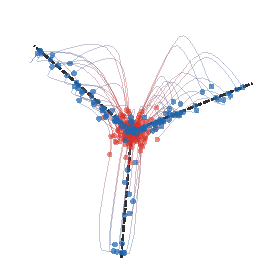
\includegraphics[width=.34\linewidth]{figures/gradflow-mlp-homogeneous-relu/neuron-trajectories.pdf} &
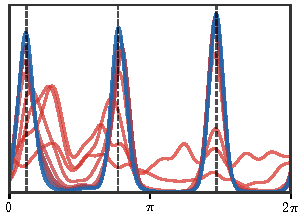
\includegraphics[width=.34\linewidth]{figures/gradflow-mlp-homogeneous-relu/direction-histogram.pdf}
\end{tabular}
\caption{\emph{Mean-field training of a homogeneous two-layer model as transport in neuron space.} The left panel shows the Wasserstein particle gradient flow in the reduced homogeneous coordinates $(|u|v_1,|u|v_2)$, with black dashed rays marking the teacher directions. The right panel shows the weighted angular density along a front-loaded sequence of times, colored from red to blue, so that the early concentration of neuron directions is visible. The display follows the rendering of the auxiliary MLP experiment but keeps only the $W_2$ flow, not the spectral-flow comparison.}
\index{two-layer neural network}% strictindex
\index{gradient!flow}% strictindex
\label{fig:gradflow-mlp-homogeneous-relu}
\end{figure}

\paragraph{Classical convexity and stationarity.}
\index{convexity!classical}% strictindex
\index{stationarity}% strictindex
Before using the specific homogeneity mechanism of Chizat and Bach, it is useful to isolate a simpler convex-analytic principle behind many mean-field arguments. Consider an energy of the form
\[
	F(\alpha)
	=
	\frac12\iint k(x,x')\d\alpha(x)\d\alpha(x')
	+
	\int V(x)\d\alpha(x)
	+C,
\]
on probability measures over a parameter domain. Assume that the quadratic part is convex in the classical sense, namely convex for the affine structure of measures:
\index{probability measure}% strictindex
\[
	Q((1-s)\alpha+s\beta)\leq (1-s)Q(\alpha)+sQ(\beta),
	\qquad
	Q(\alpha)=\frac12\iint k\d\alpha\d\alpha.
\]
This is ordinary convexity of the functional on the convex set of measures, not displacement convexity along $\Wass_2$ geodesics.
\index{convexity!along geodesics}% strictindex
\index{displacement convexity}% strictindex

\begin{prop}[Affine convexity and stationary densities]\label{prop-classical-convex-stationary}
\index{convexity!classical}% strictindex
\index{stationary density}% strictindex
	Let $F=Q+\int V\,\d\alpha+C$ be as above, and assume that $Q$ is classically convex. Suppose that a Wasserstein gradient flow for $F$ converges to a measure $\alpha_\infty=\rho_\infty\d x$. Assume also the standard regularity needed to pass to the limit in the first variation, and assume that the support and positivity of $\rho_\infty$ allow the stationary condition to be tested against all admissible zero-mass density perturbations. In the form needed here, assume that this stationarity yields, for every competitor $\beta$, the variational inequality
\index{stationary condition}% strictindex
\index{first variation}% strictindex
\index{stationarity}% strictindex
\index{Wasserstein gradient}% strictindex
\index{gradient!flow}% strictindex
\index{Wasserstein!gradient flow}% strictindex
	\[
		\int \delta F(\alpha_\infty)(x)\d(\beta-\alpha_\infty)(x)\geq0.
	\]
	Then $\alpha_\infty$ is a global minimizer of $F$.
\index{global!minimizer}% strictindex
\end{prop}
\begin{proof}[Proof sketch]
	The dissipation identity for the gradient flow gives stationarity of the limit: formally, after passing to the limit,
\index{gradient!flow}% strictindex
	\[
		\int \norm{\nabla \delta F(\alpha_\infty)}^2\d\alpha_\infty=0.
	\]
	Without such a support and positivity assumption, this identity only controls the first variation on the region explored by the limit. The density hypothesis permits testing against sufficiently many signed density perturbations of total mass zero. By approximation and the assumed regularity, this yields the displayed first-order variational inequality for arbitrary competitors $\beta$. Classical convexity of $F$ in the affine variable $\alpha$ then gives the usual subgradient inequality
\index{subgradient inequality}% strictindex
\index{first variation}% strictindex
\index{convexity!classical}% strictindex
	\[
		F(\beta)\geq F(\alpha_\infty)
		+
		\int \delta F(\alpha_\infty)\d(\beta-\alpha_\infty)
		\geq F(\alpha_\infty).
	\]
	Thus no competitor has smaller energy. For square-loss two-layer mean-field models, \eqref{eq-mlp-square-loss-quadratic-linear} is exactly of this quadratic-plus-linear form, and positive semidefiniteness of the induced kernel $k$ is the classical convexity assumption.
\index{linear form}% strictindex
\index{two-layer neural network}% strictindex
\index{convexity!classical}% strictindex
\index{classical convexity}% strictindex
\end{proof}

The convergence theory then separates two regimes. Chizat and Bach prove global convergence for the unregularized, noiseless Wasserstein flow of positively homogeneous models~\cite{ChizatBach2018OverparameterizedOT}. Mei, Montanari and Nguyen prove convergence for the noisy, regularized dynamics~\cite{MeiMontanariNguyen2018MeanFieldNN}: at the PDE level the noise adds a diffusion, or Laplacian, term, so an initially singular neuron law is immediately smoothed and acquires a density. Rotskoff and Vanden-Eijnden emphasize the parameters-as-particles interpretation, long-time convergence and asymptotic error scaling with the network width~\cite{RotskoffVandenEijnden2018Trainability}. The following formal statement isolates the noiseless Chizat--Bach mechanism and ignores the technical issues due to ReLU non-smoothness, support propagation and compactness.
\index{noisy gradient descent}% strictindex
\index{interacting particle system}% strictindex

\begin{prop}[Formal global optimality for two-homogeneous mean-field flows]\label{prop-formal-chizat-bach}
\index{global!optimality}% strictindex
	Assume that the feature is positively two-homogeneous in the neuron variable,
\index{neuron}% strictindex
	\[
		\psi(\lambda x,z)=\lambda^2\psi(x,z)
		\qquad(\lambda>0),
	\]
	and that $f(\alpha)=J(G_\alpha)$ with $J$ convex and differentiable as a functional of the predictor. Let $\alpha$ be a smooth stationary point of the Wasserstein flow, so that $\nabla_x\delta f(\alpha)(x)=0$ on $\supp(\alpha)$. Assume also full directional support: for every unit direction $\omega$, the support of $\alpha$ intersects the ray $\{\lambda\omega:\lambda>0\}$. Then $\alpha$ is a global minimizer of $f$ over the mean-field model class.
\index{stationarity}% strictindex
\index{global!minimizer}% strictindex
\end{prop}
\begin{proof}
	Choose the first-variation representative
	\[
		h_\alpha(x)=\delta f(\alpha)(x)
		=
		\left\langle \nabla J(G_\alpha),\psi(x,\cdot)\right\rangle_\rho .
	\]
	Additive constants in first variations do not affect the Wasserstein gradient or first-order inequalities between probability measures; this normalization is useful because it inherits the homogeneity of $\psi$. By two-homogeneity of $\psi$, one has
	\[
		h_\alpha(\lambda x)=\lambda^2h_\alpha(x),
		\qquad \lambda>0.
	\]
	Taking \(x=0\) and any \(\lambda\neq1\) in this identity gives \(h_\alpha(0)=0\). We first record that stationarity forces \(h_\alpha\) to vanish on \(\supp(\alpha)\). Indeed, if \(x=r\omega\in\supp(\alpha)\) with \(r>0\) and \(\norm{\omega}=1\), then
	\[
		0=\dotp{\nabla h_\alpha(r\omega)}{\omega}
		=\frac{\d}{\d s}h_\alpha(s\omega)\bigg|_{s=r}
		=2r h_\alpha(\omega),
	\]
	so \(h_\alpha(\omega)=0\), and hence \(h_\alpha(x)=r^2h_\alpha(\omega)=0\). The case \(x=0\) has already been covered, so \(h_\alpha=0\) on \(\supp(\alpha)\) and \(\int h_\alpha\,\d\alpha=0\).

	We now argue by contradiction. Suppose that a competitor \(\beta\) satisfies \(f(\beta)<f(\alpha)\). Since
	\[
		G_\beta-G_\alpha
		=
		\int \psi(x,\cdot)\d(\beta-\alpha)(x),
	\]
	convexity of \(J\) gives
	\[
		f(\beta)-f(\alpha)
		\geq
		\int h_\alpha(x)\d(\beta-\alpha)(x).
	\]
	The left-hand side is negative, while \(\int h_\alpha\,\d\alpha=0\), so \(\int h_\alpha\,\d\beta<0\). Since \(h_\alpha(0)=0\), this strict negativity must occur away from the origin: there exists a nonzero point \(x=r\omega\) with \(r>0\), \(\norm{\omega}=1\), and \(h_\alpha(x)<0\). Equivalently \(h_\alpha(\omega)=h_\alpha(x)/r^2<0\). By full directional support, there is \(r_\omega>0\) such that \(r_\omega\omega\in\supp(\alpha)\). At this support point,
	\[
		\dotp{\nabla h_\alpha(r_\omega\omega)}{\omega}
		=
		2r_\omega h_\alpha(\omega)
		<0,
	\]
	which contradicts the stationarity condition \(\nabla h_\alpha=0\) on \(\supp(\alpha)\). Thus no competitor has smaller risk.

	The rigorous Chizat--Bach theorem replaces the full directional support assumption by propagation and overparameterization hypotheses ensuring that any negative first-variation direction is represented by the evolving support. The same radial-derivative contradiction, applied after this support-propagation step, then rules out non-optimal stationary limits.
\index{stationarity}% strictindex
\end{proof}

\subsection{Generalized Dynamic Wasserstein Flows}
\label{sec-generalized-dynamic-wasserstein-flows}
\index{generalized Wasserstein flow}% strictindex
\index{dynamic!Wasserstein flow}% strictindex

This subsection explains how changing the metric geometry changes the associated descent PDE.

\paragraph{Generalized Wasserstein flows.}
\index{implicit Euler scheme}% strictindex
\index{JKO scheme}% strictindex
\index{curve of maximal slope}% strictindex
The JKO construction is not tied to the quadratic Wasserstein distance. Once a space of probability measures is equipped with a metric, an extended distance or a discrepancy \(d\) compatible with the relevant topology, one can define a minimizing movement by the implicit Euler step
\begin{equation}\label{eq-generalized-jko-step}
	\alpha_{t+\tau}
	\in
	\uargmin{\alpha}
	\frac{1}{2\tau}d^2(\alpha_t,\alpha)+f(\alpha).
\end{equation}
This is the metric-gradient-flow framework of Ambrosio, Gigli and Savar\'e~\cite{ambrosio2006gradient,gigli2011user}: under compactness, coercivity and lower-semicontinuity assumptions adapted to \(d\), the piecewise-constant interpolants of \eqref{eq-generalized-jko-step} converge, as \(\tau\to0\), to a curve of maximal slope. In the local mass-preserving examples considered below, this limiting curve is again represented by a continuity equation of the type introduced in \eqref{eq:eulerian-advection} and used for Wasserstein flows in \eqref{eq:wassflow-pde},
\begin{equation}\label{eq-generalized-flow-continuity-motivation}
	\partial_t\alpha_t+\diverg(\alpha_t v_{\alpha_t})=0,
\end{equation}
but the velocity \(v_{\alpha}\) is selected by the local steepest-descent rule associated with the geometry induced by \(d\), not necessarily by the classical \(\Wass_2\) rule. Unbalanced variants replace this continuity equation by a balance law, while nonlocal variants replace vector fields by jump fluxes.

The metric ingredient needed below is the squared-speed action $\mathbb A(\alpha,w)$ introduced in Section~\ref{sec-generalized-dynamic-wasserstein-distances}. Its length distance is already defined in~\eqref{eq-generalized-action-length-distance}; the present section only uses the local cost in the infinitesimal variational step defined below. Some actions are pointwise integrals, such as ordinary $\Wass_2$ with $\mathbb A(\alpha,w)=\int\norm w^2\d\alpha$. Others are built from a homogeneous local density but then squared at the metric level: for $\Wass_p$, the local densities are \(A_p(a,w)=a\norm w^p\) and \(J_p(a,m)=\norm m^p/a^{p-1}\), while the action paired with the JKO penalty is the squared Finsler speed
\[
	\mathbb A_p(\alpha,w)=\left(\int\norm w^p\d\alpha\right)^{2/p}.
\]
Spectral geometries use the nonlocal covariance action \(\mathbb A_\gamma\) from~\eqref{eq-spectral-tangent-action}.
In the \(\Wass_2\) case, all objects reduce to the familiar Benamou--Brenier ones:
\[
	A_2(\rho,w)=\rho\norm w^2,
	\qquad
	J_2(\rho,m)=\frac{\norm m^2}{\rho},
	\qquad
	\mathsf D_{\mathbb A}=\Wass_2.
\]
\index{local action}% strictindex
\index{tangent action}% strictindex

\begin{defn}[Penalized minimization oracle]\label{def-generalized-action-steepest-direction}
\index{penalized minimization oracle}% strictindex
\index{PMO}% strictindex
	Let \(\mathbb A(\alpha,\cdot)\) be the local squared-speed action at \(\alpha\). For a cotangent field \(u\) for which the pairing below is finite, usually \(u=\Wgrad f(\alpha)\), the penalized minimization oracle associated with this action is
	\begin{equation}\label{eq-local-action-steepest-descent}
		\operatorname{PMO}_{\mathbb A,\alpha}(u)
		\in
		\uargmin{w}
		\left\{
		\int \dotp{u(x)}{w(x)}\d\alpha(x)
		+
		\frac12\mathbb A(\alpha,w)
		\right\},
	\end{equation}
	where the minimization is over admissible finite-action velocity representatives for the chosen geometry. In Hilbertian examples \(u\in L^2(\alpha;\RR^d)\); for \(\Wass_p\), the natural dual space is \(L^q(\alpha;\RR^d)\), with \(q=p/(p-1)\).
\end{defn}

For an energy $f$, the formal small-step expansion of the generalized JKO step~\eqref{eq-generalized-jko-step}, when the distance is generated by the squared-speed action \(\mathbb A\), selects the PMO direction
\begin{equation}\label{eq-generalized-gradient-from-action}
	v_{\alpha}
	=
	\operatorname{PMO}_{\mathbb A,\alpha}(\Wgrad f(\alpha)).
\end{equation}
Equivalently, the formal evolution is
\begin{equation}\label{eq-local-action-gradient-flow-pde}
	\partial_t\alpha_t
	+
	\diverg\!\left(
	\alpha_t\,\operatorname{PMO}_{\mathbb A,\alpha_t}(\Wgrad f(\alpha_t))
	\right)=0.
\end{equation}
If \(w\mapsto\mathbb A(\alpha,w)\) has zero-action directions, the minimization in~\eqref{eq-local-action-steepest-descent} is understood on the quotient tangent space, or after projecting onto finite-action directions modulo the kernel of \(\mathbb A(\alpha,\cdot)\). Along smooth solutions of~\eqref{eq-local-action-gradient-flow-pde}, whenever the minimizer is attained and \(w\mapsto\mathbb A(\alpha,w)\) is \(2\)-homogeneous, one obtains the dissipation identity
\[
	\frac{\d}{\d t}f(\alpha_t)
	=
	\left\langle \Wgrad f(\alpha_t),v_t\right\rangle_{\alpha_t}
	=
	-\mathbb A(\alpha_t,v_t),
	\qquad
	v_t=\operatorname{PMO}_{\mathbb A,\alpha_t}(\Wgrad f(\alpha_t)).
\]
\index{normalized gradient flow}% strictindex

For \(\Wass_2\), \(\mathbb A(\alpha,w)=\int\norm w^2\d\alpha\) and \(\operatorname{PMO}_{\mathbb A,\alpha}(u)=-u\). Hence~\eqref{eq-local-action-gradient-flow-pde} reduces to the standard Wasserstein gradient-flow equation
\[
	\partial_t\alpha_t
	=
	\diverg\!\left(\alpha_t\Wgrad f(\alpha_t)\right),
\]
which is the convention used throughout the preceding sections.

In the restricted Riemannian case of~\eqref{eq-general-quadratic-tangent-action}, where
\[
	\mathbb A(\alpha,w)=\left\langle Q_\alpha w,w\right\rangle_{L^2(\alpha)},
\]
the PMO becomes the linear preconditioning rule
\begin{equation}\label{eq-generalized-gradient-q-preconditioner}
	\operatorname{PMO}_{\mathbb A,\alpha}(u)
	=
	-Q_\alpha^{-1}u,
	\qquad
	v_\alpha=-Q_\alpha^{-1}\Wgrad f(\alpha).
\end{equation}
The linear inverse formula is special to Hilbertian actions. A basic non-Hilbertian example is \(\Wass_p\): for \(1<p<+\infty\), the squared Finsler tangent action associated with the distance is
\[
	\mathbb A_p(\alpha,w)=\left(\int\norm{w}^p\d\alpha\right)^{2/p}.
\]
Writing \(q=p/(p-1)\) and \(U=\norm{u}_{L^q(\alpha)}\), its PMO is the duality-map formula
\begin{equation}\label{eq-wp-pmo}
	\operatorname{PMO}_{\mathbb A_p,\alpha}(u)(x)
	=
	-\,U^{2-q}\norm{u(x)}^{q-2}u(x),
\end{equation}
with the conventions that the right-hand side is \(0\) when \(U=0\), and that \(\norm{u(x)}^{q-2}u(x)=0\) when \(u(x)=0\). This is nonlinear in \(u\), and it reduces to \(-u\) only for \(p=2\). Endpoint cases such as \(p=1\) are interpreted through subgradients of the dual norm.

The examples below are organized by the same dictionary. Concave-mobility flows use $\mathbb A_{\theta,\lambda}(\alpha,v)$ from Section~\ref{rem-generalized-bb}; spectral flows use $\mathbb A_\gamma(\alpha,v)$ from~\eqref{eq-spectral-tangent-action}; kernelized Benamou--Brenier flows use $\mathbb A_k(\alpha,v)=\norm{v}_{\RKHS_k^d}^2$ with a restricted RKHS tangent space. Nonlocal logarithmic-mean geometries also have quadratic actions, but their tangent variables are edge potentials or jump velocities rather than vector fields in $\RR^d$; their flows are treated separately in Section~\ref{sec-nonlocal-wasserstein-flows}. WFR, defined by~\eqref{eq-dynamic-unbalanced-ot} and studied separately in Section~\ref{sec-wfr-gradient-flows}, is another quadratic geometry, but its tangent variable is a pair $(v,g)$ combining displacement and mass modulation.

The generalized distances of Section~\ref{sec-generalized-dynamic-wasserstein-distances} are useful precisely because they change what \emph{descent} means. The energy functional can be the same, while the local metric tensor, Finsler norm, mobility, spectral gauge or RKHS constraint changes the PDE selected by the minimizing movement. The rest of this section focuses on local or vector-field mass-preserving geometries. Nonlocal pair-space geometries are separated in Section~\ref{sec-nonlocal-wasserstein-flows}, and the transport--reaction case is separated in Section~\ref{sec-wfr-gradient-flows}, because their tangent variables are structurally different.

\paragraph{General mobility flows.}
\index{mobility}% strictindex
\index{concave mobility}% strictindex
The concave-mobility distances of Section~\ref{rem-generalized-bb} replace the scalar linear mobility \(a\) by a concave mobility \(\theta(a)\). For a density field \(a=\rho_t(x)\), this changes the Onsager operator of the gradient flow while keeping a continuity equation.

Let \(\lambda\) be Lebesgue measure, write \(\alpha=\rho\lambda\), and let \(u=\nabla(\delta F/\delta\rho)\). For the velocity action \(\mathbb A_{\theta,\lambda}\), the PMO introduced in Definition~\ref{def-generalized-action-steepest-direction} is the pointwise minimizer of
\[
\int \dotp{u}{w}\,\rho\,\d x
+
\frac12\int \frac{\rho}{\theta(\rho)}\norm{w}^2\rho\,\d x,
\]
so, wherever \(\rho>0\) and \(\theta(\rho)>0\),
\begin{equation}\label{eq-concave-mobility-pmo}
\operatorname{PMO}_{\mathbb A_{\theta,\lambda},\rho\lambda}(u)
=
-\frac{\theta(\rho)}{\rho}u.
\end{equation}
Thus the flux \(\rho w\) is \(-\theta(\rho)\nabla(\delta F/\delta\rho)\). For a smooth density \(\rho_t\) and an energy \(F\), the formal gradient flow associated with the pointwise momentum action \(J_\theta(a,m)=|m|^2/\theta(a)\) is
\begin{equation}\label{eq-general-mobility-gradient-flow}
	\partial_t\rho_t
	=
	\nabla\!\cdot\!\left(\theta(\rho_t)\nabla\frac{\delta F}{\delta\rho}(\rho_t)\right).
\end{equation}
If
\[
	F(\rho)=\int U(\rho(x))\,\d x+\int V(x)\rho(x)\,\d x,
\]
then \eqref{eq-general-mobility-gradient-flow} becomes
\[
	\partial_t\rho
	=
	\nabla\!\cdot\!\left(\theta(\rho)\big(U''(\rho)\nabla\rho+\nabla V\big)\right).
\]
Thus \(\theta(a)=a\) and \(U(a)=a\log a\) gives the usual heat or Fokker--Planck equation, while \(\theta(a)=a(1-a/M)\) gives a volume-filling drift--diffusion whose mobility vanishes at saturation. Power internal energies and power mobilities tune nonlinear diffusion: for instance \(\theta(a)=a\) and \(U(a)=a^m/(m-1)\) yield \(\partial_t\rho=\Delta(\rho^m)\), whereas the entropy with \(\theta(a)=a^\gamma\), \(0<\gamma<1\), gives the fast-diffusion-type equation \(\partial_t\rho=(1/\gamma)\Delta(\rho^\gamma)\). This viewpoint is useful for nonlinear diffusions, exclusion models, volume-filling models and finite-volume discretizations~\cite{dolbeault2009new}; vector-valued and dissipative extensions follow the same principle but use richer mobility tensors.
\index{Fokker-Planck equation}% strictindex
\index{porous medium equation}% strictindex
\index{fast diffusion equation}% strictindex

\paragraph{Dynamic spectral Wasserstein flows.}\label{sec-normalized-spectral-wasserstein-dynamics}
\index{normalized gradient flow}% strictindex
\index{normalized dynamics}% strictindex
\index{spectral Wasserstein flow}% strictindex
\index{spectral steepest descent}% strictindex
\index{Muon algorithm}% strictindex

The spectral tangent action \eqref{eq-spectral-tangent-action}, and the dynamic distance \eqref{eq-dynamic-spectral-wasserstein} it generates, normalize the whole velocity covariance through a monotone spectral gauge. Using this geometry for gradient descent replaces the pointwise Wasserstein direction by a globally preconditioned direction. This is close to many large-scale optimizers: normalized gradient methods solve norm-constrained linear minimization problems~\cite{PethickXieAntonakopoulosEtAl2025}; related ideas appear in normalized SGD~\cite{MurraySwensonKar2019,CutkoskyMehta2020}, tensor-aware optimizers such as Shampoo~\cite{GuptaKorenSinger2018}, and Muon-type spectral normalizations~\cite{KellerJordan2024,LiuSuYaoEtAl2025}. We now describe the mean-field version developed in~\cite{peyre2026muon}. The trace gauge gives the classical $\Wass_2$ flow, while the operator gauge $\gamma(M)=\lambda_{\max}(M)$ gives the idealized Muon geometry.
\index{normalized SGD}% strictindex
\index{Shampoo optimizer}% strictindex
\index{spectral gauge}% strictindex
\index{operator gauge}% strictindex

Specializing Definition~\ref{def-generalized-action-steepest-direction} to the spectral action \(\mathbb A_\gamma\), the descent direction associated with a field \(g\in L^2(\alpha;\RR^d)\) is simply \(\operatorname{PMO}_{\mathbb A_\gamma,\alpha}(g)\).
The field \(g\) should be read as the Wasserstein gradient \(g=\Wgrad f(\alpha)=\nabla\delta f(\alpha)\). Since \(v\mapsto\mathbb A_\gamma(\alpha,v)\) is \(2\)-homogeneous, fixed-speed normalized algorithms keep the same ray as this PMO and only change the scalar normalization; equivalently, they minimize the linear pairing over the unit ball \(\mathbb A_\gamma(\alpha,w)\leq1\). In the trace case, \(\mathbb A_{\tr}(\alpha,v)=\int\norm{v}^2\d\alpha\) and \(\operatorname{PMO}_{\mathbb A_{\tr},\alpha}(g)=-g\). For other gauges, the velocity is globally preconditioned by the covariance of \(g\) under \(\alpha\).
\index{spectral tangent action}% strictindex

\begin{prop}[Polar formula for the spectral direction]\label{prop-normalized-spectral-polar}
\index{polar set}% strictindex
	Let
	\[
		S_\alpha(g)\eqdef\int g(x)g(x)^\top\d\alpha(x).
	\]
	Assume that the inverse-trace problem admits a positive definite minimizer
	\[
		A_\alpha^\star
		\in
		\uargmin{A\in\mathcal B_\gamma\cap\mathbb S_{++}^d}
		\tr\!\left(A^{-1}S_\alpha(g)\right).
	\]
	Then
	\begin{equation}\label{eq-normalized-spectral-direction-explicit}
		\operatorname{PMO}_{\mathbb A_\gamma,\alpha}(g)(x)
		=
		-(A_\alpha^\star)^{-1}g(x)
	\end{equation}
	is the spectral PMO direction. If the minimizer lies on the boundary of $\mathcal B_\gamma$, the same formula is understood by a limiting argument along positive definite minimizers, or equivalently by replacing the inverse by the corresponding inverse on the range of $S_\alpha(g)$.
\end{prop}
\begin{proof}
	Using the polar formula $\gamma(M)=\sup_{A\in\mathcal B_\gamma}\tr(AM)$, the PMO objective~\eqref{eq-local-action-steepest-descent} with \(\mathbb A=\mathbb A_\gamma\) can be written as
	\[
		\sup_{A\in\mathcal B_\gamma}
		\left\{
		\int \dotp{g}{v}\d\alpha
		+
		\frac12\int v^\top A v\d\alpha
		\right\}.
	\]
	For a fixed $A\succ0$, the quadratic lower bound
	\[
		\int \dotp{g}{v}\d\alpha+\frac12\int v^\top A v\d\alpha
	\]
	is minimized by $v_A=-A^{-1}g$, with value $-\frac12\tr(A^{-1}S_\alpha(g))$. Let $v_\star=-(A_\alpha^\star)^{-1}g$ and
	\[
		M_\star=\int v_\star(x)v_\star(x)^\top\d\alpha(x)
		=
		(A_\alpha^\star)^{-1}S_\alpha(g)(A_\alpha^\star)^{-1}.
	\]
	Since $A_\alpha^\star$ minimizes $A\mapsto\tr(A^{-1}S_\alpha(g))$ over the convex polar set, its first-order optimality condition gives
	\[
		\tr(AM_\star)\leq \tr(A_\alpha^\star M_\star)
		\qquad
		\text{for all } A\in\mathcal B_\gamma.
	\]
	Thus $A_\alpha^\star$ is active in the polar representation of $\gamma(M_\star)$, and
	\[
		\gamma(M_\star)=\tr(A_\alpha^\star M_\star)
		=
		\tr((A_\alpha^\star)^{-1}S_\alpha(g)).
	\]
	For any $v$, the polar formula gives
	\[
		\int \dotp{g}{v}\d\alpha+\frac12\mathbb A_\gamma(\alpha,v)
		\geq
		\int \dotp{g}{v}\d\alpha+\frac12\int v^\top A_\alpha^\star v\d\alpha,
	\]
	and the right-hand side is minimized at $v_\star$. The activity identity above shows that equality holds at $v_\star$, hence $v_\star$ is the spectral PMO direction. The boundary case follows by approximation with positive definite matrices in the polar set.
\end{proof}

For the trace gauge, $\mathcal B_\gamma=\enscond{A}{0\preceq A\preceq\Id}$ and the minimizer is $A_\alpha^\star=\Id$. For the operator gauge $\gamma(M)=\lambda_{\max}(M)$, one has $\mathcal B_\gamma=\enscond{A\succeq0}{\tr(A)\leq1}$; if $S_\alpha(g)\succ0$, then
\[
	A_\alpha^\star
	=
	\frac{S_\alpha(g)^{1/2}}{\tr(S_\alpha(g)^{1/2})},
	\qquad
	\operatorname{PMO}_{\mathbb A_\gamma,\alpha}(g)(x)
	=
	-\tr(S_\alpha(g)^{1/2})\,S_\alpha(g)^{-1/2}g(x).
\]
This is the continuum covariance-normalization formula that becomes the Muon polar factor for empirical measures.
\index{covariance normalization}% strictindex
\index{Muon polar factor}% strictindex

\index{JKO scheme}% strictindex
\index{minimizing movement}% strictindex
The static/dynamic equality of Proposition~\ref{prop-static-dynamic-spectral-wasserstein} implies that the same local action \(\mathbb A_\gamma(\alpha,v)\) is obtained either from the dynamic path-length geometry \eqref{eq-dynamic-spectral-wasserstein} or from the small-step expansion of the static distance \(\Wass_\gamma\). Therefore the spectral flow is the general JKO scheme~\eqref{eq-generalized-jko-step} with \(d=\Wass_\gamma\). For a small displacement $\alpha=(\Id+\tau v)_\sharp\alpha^k$, the tangent expansion is
\[
	\Wass_\gamma(\alpha^k,(\Id+\tau v)_\sharp\alpha^k)^2
	=
	\tau^2\mathbb A_\gamma(\alpha^k,v)+o(\tau^2).
\]
Combining this with the first-variation expansion of $f$ gives precisely the general PMO problem~\eqref{eq-local-action-steepest-descent} specialized to the spectral action \(\mathbb A_\gamma\).

\begin{prop}[Formal normalized spectral gradient flow]\label{prop-normalized-spectral-gradient-flow}
\index{spectral Wasserstein flow}% strictindex
\index{continuity equation}% strictindex
	Assume that $f$ has a smooth first variation and that the tangent expansion of $\Wass_\gamma$ above is valid along smooth perturbations. Then the formal small-step limit of the general JKO scheme~\eqref{eq-generalized-jko-step} with \(d=\Wass_\gamma\), equivalently \eqref{eq-local-action-gradient-flow-pde} with \(\mathbb A(\alpha,v)=\mathbb A_\gamma(\alpha,v)\), solves
	\begin{equation}\label{eq-normalized-spectral-flow}
		\partial_t\alpha_t
		+
		\diverg\!\left(
		\alpha_t\,\operatorname{PMO}_{\mathbb A_\gamma,\alpha_t}(\Wgrad f(\alpha_t))
		\right)=0.
	\end{equation}
	Equivalently, if $A_t^\star$ solves the inverse-trace problem for
	\[
		S_t=\int \Wgrad f(\alpha_t)(x)\Wgrad f(\alpha_t)(x)^\top\d\alpha_t(x),
	\]
	then the velocity is
	\[
		v_t(x)=-(A_t^\star)^{-1}\Wgrad f(\alpha_t)(x).
	\]
	Moreover, along smooth solutions,
	\[
		\frac{\d}{\d t}f(\alpha_t)
		=
		-\mathbb A_\gamma(\alpha_t,v_t).
	\]
\end{prop}
\begin{proof}
	Write $\alpha=(\Id+\tau v)_\sharp\alpha_t$. The spectral JKO objective equals, up to terms independent of $v$ and $o(\tau)$,
	\[
		\tau\left[
		\frac12\mathbb A_\gamma(\alpha_t,v)
		+
		\int\dotp{\Wgrad f(\alpha_t)(x)}{v(x)}\d\alpha_t(x)
		\right].
	\]
	Minimizing the bracket gives \(v=\operatorname{PMO}_{\mathbb A_\gamma,\alpha_t}(\Wgrad f(\alpha_t))\). Substituting this velocity into the transport expansion
	\[
		(\Id+\tau v)_\sharp\alpha_t
		=
		\alpha_t-\tau\diverg(\alpha_t v)+o(\tau)
	\]
	gives \eqref{eq-normalized-spectral-flow}.
	Finally, the variation formula gives $\frac{\d}{\d t}f(\alpha_t)=\int\dotp{\Wgrad f(\alpha_t)}{v_t}\d\alpha_t$. Since $v_t$ minimizes a $2$-homogeneous penalized objective, the one-dimensional rescaling $s\mapsto sv_t$ has derivative zero at $s=1$, hence
	\[
		\int\dotp{\Wgrad f(\alpha_t)}{v_t}\d\alpha_t
		+
		\mathbb A_\gamma(\alpha_t,v_t)
		=0,
	\]
	which proves the dissipation identity.
\end{proof}

\begin{rem}[Empirical and Muon limits]
\index{empirical!measure}% strictindex
\index{Muon algorithm}% strictindex
For empirical measures $\alpha_X=n^{-1}\sum_i\delta_{x_i}$, stack the velocities $v(x_i)$ into a matrix $V\in\RR^{n\times d}$ and the gradients $g(x_i)$ into a matrix $G\in\RR^{n\times d}$. By $1$-homogeneity of $\gamma$,
\[
	\mathbb A_\gamma(\alpha_X,v)
	=
	\gamma\!\left(\frac1n V^\top V\right)
	=
	\frac1n\gamma(V^\top V),
	\qquad
	\int\dotp{g}{v}\d\alpha_X
	=
	\frac1n\tr(G^\top V).
\]
Thus the empirical specialization of the PMO problem~\eqref{eq-local-action-steepest-descent} is, up to the harmless factor $1/n$, the finite-dimensional matrix descent problem. Writing
\[
	(G_X(t))_i=\Wgrad f(\alpha_{X(t)})(x_i(t)),
\]
the empirical flow is
\begin{equation}\label{eq-normalized-matrix-descent}
	\dot X(t)
	\in
	\uargmin{V\in\RR^{n\times d}}
	\left\{
		\tr(G_X(t)^\top V)+\frac12\gamma(V^\top V)
	\right\}.
\end{equation}
Here $G_X$ is the gradient for the empirical Wasserstein metric $\norm{\dot X}_n^2=n^{-1}\sum_i\norm{\dot x_i}^2$, not the ordinary Euclidean gradient of $f(\alpha_X)$. If one rewrites the same rule with the unweighted matrix convention, it corresponds to the lift $X\mapsto n f(\alpha_X)$; using $X\mapsto f(\alpha_X)$ only rescales time by the factor $n$.
If $G=U\diag(\sigma_i)W^\top$ and $\gamma(M)=\lambda_{\max}(M)$, then
\begin{equation}\label{eq-normalized-muon-direction}
	\uargmin{V\in\RR^{n\times d}}
	\left\{
		\tr(G^\top V)+\frac12\lambda_{\max}(V^\top V)
	\right\}
	\ni
	-\norm{G}_{S_1}UW^\top
	=
	-\tr\!\left((G^\top G)^{1/2}\right)G(G^\top G)^{\dagger/2}.
\end{equation}
The ray of this direction is the polar factor $-UW^\top$, and the scalar factor $\norm{G}_{S_1}$ can be absorbed into a time or step-size normalization. This is the exact-polar, full-batch, continuous-time idealization of Muon~\cite{KellerJordan2024,peyre2026muon}. Practical Muon implementations replace the polar factor by a few Newton--Schulz iterations for GPU efficiency~\cite{LiuSuYaoEtAl2025}; this polynomial approximation fits the same spectral-normalization philosophy, although adaptive rescaling and finite momentum make the practical algorithm more than a position-only metric gradient flow.
\index{step-size normalization}% strictindex
\index{Newton--Schulz iteration}% strictindex
\index{polar factor}% strictindex
\end{rem}

The effect of this spectral normalization is visible already in the homogeneous two-layer ReLU model discussed in Section~\ref{sec-wasserstein-flows-mlp}. Figure~\ref{fig:gradflow-mlp-w2-vs-muon} reproduces, in the style of the book figures, the numerical comparison from~\cite{peyre2026muon}: the same teacher network, same initialization and same empirical first variation are evolved either by the $W_2$ particle flow or by the operator-gauge Muon direction.

\begin{figure}[H]
\centering
\begin{tabular}{@{}ccc@{}}
\scriptsize $W_2$ trajectories & \scriptsize Muon trajectories & \scriptsize risk decay \\[-.15em]
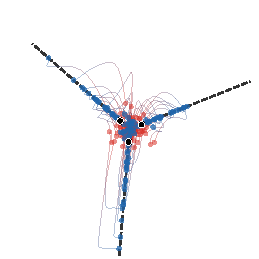
\includegraphics[width=.285\linewidth]{figures/gradflow-mlp-w2-vs-muon/trajectories-w2.pdf} &
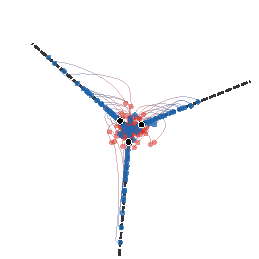
\includegraphics[width=.285\linewidth]{figures/gradflow-mlp-w2-vs-muon/trajectories-muon.pdf} &
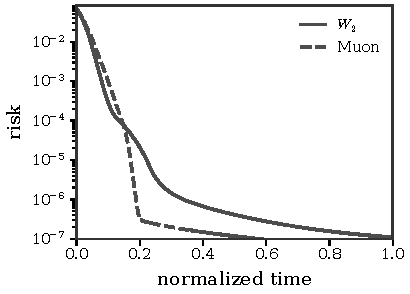
\includegraphics[width=.345\linewidth]{figures/gradflow-mlp-w2-vs-muon/risk-comparison.pdf}
\end{tabular}
\caption{\emph{Wasserstein versus Muon mean-field training of a homogeneous ReLU model.} The first two panels display trajectories in the reduced homogeneous coordinates $(|u|v_1,|u|v_2)$; black dashed rays are the teacher directions. The right panel compares the empirical square-loss decay, with the solid curve for the $W_2$ flow and the dashed curve for the operator-gauge Muon flow. Both methods use the same particles and first variation; the spectral normalization reaches the low-risk regime earlier in normalized time.}
\index{Muon algorithm}% strictindex
\index{two-layer neural network}% strictindex
\index{spectral Wasserstein flow}% strictindex
\label{fig:gradflow-mlp-w2-vs-muon}
\end{figure}

\subsection{Nonlocal Wasserstein Flows}
\label{sec-nonlocal-wasserstein-flows}
\label{sec-nonlocal-wasserstein-pdes}
\index{nonlocal Wasserstein flow}% strictindex
\index{fractional PDE}% strictindex
\index{Markov-chain Wasserstein geometry}% strictindex

The nonlocal distances of Section~\ref{sec-nonlocal-wasserstein-distances} replace the local vector-field tangent model by pairwise exchanges. This separate section records the corresponding gradient-flow interpretation in the same order as the distance constructions: first continuum nonlocal Wasserstein flows and fractional PDEs, then discrete Wasserstein flows on Markov chains. In the continuum jump-kernel case, entropy descent gives nonlocal diffusion and, for power-law kernels, fractional PDEs. On a finite state space, the same logarithmic-mean edge calculus makes a reversible Markov chain exactly the entropy gradient flow of the discrete Wasserstein distance. Both examples are mass-preserving, but they are not local Benamou--Brenier flows: their tangent variables live on pairs or graph edges rather than at individual points.

\paragraph{Nonlocal Wasserstein flows and fractional PDEs.}
\index{nonlocal Wasserstein distance}% strictindex
\index{jump process}% strictindex
\index{fractional Laplacian}% strictindex

The continuum nonlocal distance \(\mathcal W_K\) of Section~\ref{sec-nonlocal-wasserstein-distances} replaces local velocities by antisymmetric fluxes across jumps selected by a reversible kernel \(K\). Its logarithmic-mean mobility is chosen so that entropy dissipation produces the Markov generator. This turns jump processes, fractional heat equations and some heavy-tailed stochastic models into gradient flows for nonlocal transport geometries.
\index{transport metric}% strictindex
\index{Markov-chain Wasserstein geometry}% strictindex
\index{antisymmetric flux}% strictindex

\begin{prop}[Entropy gradient flow for reversible jump kernels]\label{prop-nonlocal-entropy-gradient-flow}
\index{relative entropy}% strictindex
\index{Markov semigroup}% strictindex
	Under the regularity and irreducibility assumptions used in Proposition~\ref{prop-nonlocal-distance-properties}, the Markov semigroup generated by the closure of
	\[
		L\psi(x)
		=
		\int\bigl(\psi(y)-\psi(x)\bigr)K(x,\d y)
	\]
	is the gradient flow, for the distance \(\mathcal W_K\) defined in \eqref{eq-nonlocal-wasserstein-distance}, of the relative entropy
	\[
		\mathrm{Ent}_{\mathfrak m}(\alpha)
		=
		\int \rho\log\rho\,\d\mathfrak m,
		\qquad
		\alpha=\rho\mathfrak m.
	\]
	Equivalently, in weak form, the entropy flow is
	\begin{equation}\label{eq-nonlocal-entropy-flow}
		\partial_t\rho_t=L\rho_t .
	\end{equation}
	When \(K\) is singular, the integral defining \(L\) is understood in the principal-value sense.
\end{prop}

\begin{proof}[Proof idea]
	The key identity is the logarithmic-mean relation
	\[
		\theta(a,b)(\log a-\log b)=a-b.
	\]
	The first variation of \(\mathrm{Ent}_{\mathfrak m}\) is \(\log\rho+1\). With the sign convention of \eqref{eq-nonlocal-continuity-weak}, the steepest descent velocity is
	\[
		v(x,y)
		=
		-\bar\nabla(\log\rho+1)(x,y)
		=
		\log\rho(x)-\log\rho(y).
	\]
	Hence \(\theta(\rho(x),\rho(y))v(x,y)=\rho(x)-\rho(y)\). Substituting this in \eqref{eq-nonlocal-continuity-weak} and using the symmetry of \(\mathsf J\) gives
	\[
		\frac{\d}{\d t}\int \varphi\rho\,\d\mathfrak m
		=
		\int \varphi(x)\int(\rho(y)-\rho(x))K(x,\d y)\,\mathfrak m(\d x),
	\]
	which is the weak form of \(\partial_t\rho=L\rho\). The metric properties needed to justify this computation as a gradient-flow identity are the distance and geodesic results recalled in Proposition~\ref{prop-nonlocal-distance-properties}.
\end{proof}

\index{fractional diffusion}% strictindex
\index{stable process}% strictindex
\index{power-law jump kernel}% strictindex
The construction becomes especially transparent for translation-invariant kernels. A power-law jump kernel turns the entropy flow into a fractional heat equation.

On \(\mathcal X=\RR^d\), let
\[
	K_s(x,\d y)
	=
	c_{d,s}\frac{\d y}{|x-y|^{d+s}},
	\qquad
	0<s<2.
\]
The associated generator is, up to the normalizing constant,
\index{principal value}% strictindex
\index{fractional Laplacian}% strictindex
\[
	L_s\psi(x)
	=
	\mathrm{p.v.}\int_{\RR^d}
	\bigl(\psi(y)-\psi(x)\bigr)
	\frac{c_{d,s}}{|x-y|^{d+s}}\,\d y
	=
	-(-\Delta)^{s/2}\psi(x),
\]
where \((-\Delta)^{s/2}\) is the fractional Laplacian~\cite{samko1993fractional}. Hence the \(\mathcal W_{K_s}\)-gradient flow of the entropy is
\begin{equation}\label{eq-fractional-heat-nonlocal-wasserstein}
	\partial_t\rho_t
	=
	-(-\Delta)^{s/2}\rho_t .
\end{equation}
Figure~\ref{fig:gradflow-fractional-laplacian-diffusion} illustrates the qualitative effect of lowering \(s\). Classical heat diffusion, \(s=2\), smooths local discontinuities by nearby averaging. Fractional diffusion keeps a sharper memory of localized peaks but immediately creates algebraic long-range tails, because mass can jump over macroscopic distances.

\begin{figure}[ht]
\centering
\begin{tabular}{@{}ccc@{}}
\small classical heat, \(s=2\) & \small medium nonlocality, \(s=0.85\) & \small strong nonlocality, \(s=0.35\) \\[-.15em]
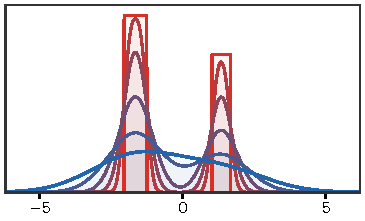
\includegraphics[width=.30\linewidth]{figures/gradflow-fractional-laplacian-diffusion/classical.pdf} &
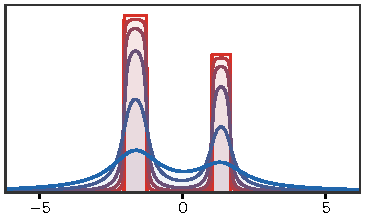
\includegraphics[width=.30\linewidth]{figures/gradflow-fractional-laplacian-diffusion/nonlocal-medium.pdf} &
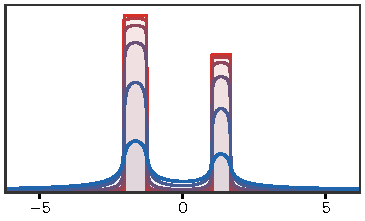
\includegraphics[width=.30\linewidth]{figures/gradflow-fractional-laplacian-diffusion/nonlocal-strong.pdf}
\end{tabular}
\caption{\emph{Classical and fractional heat flows from two localized indicator bumps.} Each panel evolves the same normalized mixture of two intervals by the Fourier multiplier \(e^{-t|\xi|^s}\), with time colored from red to blue. The classical heat flow quickly rounds the discontinuities and spreads by local Gaussian averaging. As \(s\) decreases, the diffusion becomes increasingly nonlocal: peaks remain more localized near the bumps, while heavier tails appear across the whole displayed window.}
\index{fractional Laplacian}% strictindex
\index{fractional heat equation}% strictindex
\label{fig:gradflow-fractional-laplacian-diffusion}
\end{figure}

More generally, when a target-dependent jump kernel \(K_\beta\) satisfies detailed balance with a desired invariant measure \(\beta=\rho_\beta\mathfrak m\), the same construction can be applied to \(r_t=\d\alpha_t/\d\beta\). The gradient flow of \(\KL(\alpha|\beta)\) is then \(\partial_t r_t=L_\beta r_t\). This is the nonlocal analogue of the Fokker--Planck gradient flow of relative entropy, and it is one of the motivations behind more recent nonlocal diffusion gradient-flow frameworks~\cite{Warren2024NonlocalDiffusionGradientFlow}.
\index{fractional heat equation}% strictindex
\index{Fokker-Planck equation}% strictindex

\begin{rem}[L\'evy SDE viewpoint]
\index{Levy process}% strictindex
\index{stochastic differential equation}% strictindex
The same operators appear probabilistically as generators of jump processes. This gives a complementary interpretation of nonlocal PDEs as laws of stochastic processes with heavy-tailed jumps.

For the kernel \(K_s\), the process with generator \(L_s\) is the symmetric \(s\)-stable L\'evy process \(X_t=X_0+L_t^{(s)}\), whose density solves \eqref{eq-fractional-heat-nonlocal-wasserstein}~\cite{Applebaum2009Levy}. Adding a smooth confining drift gives the fractional Fokker--Planck equation
\begin{equation}\label{eq-fractional-fokker-planck}
	\partial_t\rho_t
	=
	\nabla\cdot(\rho_t\nabla V)
	-
	\sigma^s(-\Delta)^{s/2}\rho_t,
\end{equation}
which is the forward equation of
\[
	\d X_t=-\nabla V(X_t)\,\d t+\sigma\,\d L_t^{(s)}.
\]
Equation~\eqref{eq-fractional-fokker-planck} should be distinguished from the exactly reversible entropy flow above unless the jump kernel is chosen to satisfy detailed balance with the target measure. Both viewpoints, however, share the same nonlocal mechanism: relaxation is driven not only by local drift and Brownian diffusion but also by rare long jumps.
\index{detailed balance}% strictindex
\index{fractional Fokker-Planck equation}% strictindex
\end{rem}

\begin{rem}[Connection with stochastic gradient dynamics]
\index{stochastic gradient descent}% strictindex
\index{gradient noise}% strictindex
\index{heavy-tailed noise}% strictindex
This nonlocal point of view is useful in machine learning because stochastic optimization noise need not be well approximated by Brownian noise. Classical diffusion approximations model small-step SGD by a Brownian SDE near stationarity~\cite{MandtHoffmanBlei2017SGD}. In deep-network regimes, empirical and theoretical work has shown that gradient noise and even stationary iterates can be heavy-tailed~\cite{SimsekliSagunGurbuzbalaban2019TailIndex,GurbuzbalabanSimsekliZhu2021HeavyTailSGD}. A coarse continuous-time model for parameters \(\Theta_t\) is then
\[
	\d\Theta_t
	=
	-\nabla \mathcal L(\Theta_t)\,\d t
	+
	\sigma\,\d L_t^{(s)},
\]
whose law solves a fractional Fokker--Planck equation of the form \eqref{eq-fractional-fokker-planck}. The jumps represent occasional large stochastic-gradient fluctuations, so they can move the dynamics between basins in a way that Brownian approximations tend to understate. This makes nonlocal Wasserstein geometries a useful language for linking heavy-tailed training noise, fractional PDE models, and measure-valued gradient-flow ideas. The correspondence remains a modeling approximation: the effective tail index, anisotropy, minibatch correlations and learning-rate schedule all influence whether a L\'evy limit is a faithful description of a concrete training run.
\index{tail index}% strictindex
\index{minibatch noise}% strictindex
\end{rem}

\paragraph{Discrete Wasserstein flows on Markov chains.}
\index{Markov-chain Wasserstein geometry}% strictindex
\index{discrete Wasserstein geometry}% strictindex
\index{Markov semigroup}% strictindex
The finite-state distance \(\mathcal W_K\) in Section~\ref{sec-discrete-wasserstein-markov} is designed so that the reversible Markov chain itself becomes an entropy gradient flow. This is the discrete counterpart of the fact that the heat equation is the Wasserstein gradient flow of Shannon entropy.

For masses \(a_i=\pi_i\rho_i\), or equivalently relative densities \(\rho_i=a_i/\pi_i\) with respect to the invariant law \(\pi\), the entropy relative to \(\pi\) is
\[
\operatorname{Ent}_\pi(\rho)\eqdef\sum_i\pi_i\rho_i\log\rho_i.
\]
Applying the general minimizing movement~\eqref{eq-generalized-jko-step} with \(d=\mathcal W_K\) and \(f=\operatorname{Ent}_\pi\), the small-\(\tau\) first-order optimality condition gives
\[
\frac{\rho^{k+1}-\rho^k}{\tau}
=-\mathcal K_{\rho^k}\log\rho^k+O(\tau)
=K\rho^k+O(\tau),
\]
where \((K\rho)_i=\sum_jK_{ij}(\rho_j-\rho_i)\). Thus the discrete Wasserstein geometry is engineered so that the entropy gradient flow is the Markov semigroup; the proposition below makes this identity explicit.
\index{JKO scheme}% strictindex

\begin{prop}[Entropy gradient flow of a reversible Markov chain]
\label{prop-discrete-markov-entropy-gradient}
Let \(K\) be reversible with invariant law \(\pi\). The gradient flow of \(\operatorname{Ent}_\pi\) for the metric \(\mathcal W_K\) is the forward equation of the Markov chain,
\index{Markov chain}% strictindex
\begin{equation}
\label{eq-discrete-markov-gradient-flow}
\dot\rho_i(t)=\sum_jK_{ij}\bigl(\rho_j(t)-\rho_i(t)\bigr).
\end{equation}
Equivalently, for the masses \(a_i(t)=\pi_i\rho_i(t)\), this is \(\dot a_i(t)=\sum_j(a_j(t)K_{ji}-a_i(t)K_{ij})\).
\end{prop}

\begin{proof}
The first variation of the entropy, with respect to the weighted pairing \(\sum_i\pi_i\xi_i\varphi_i\), is \(\log\rho_i+1\). Constants do not contribute to \(\mathcal K_\rho\), hence the metric gradient-flow equation is
\[
\dot\rho=-\mathcal K_\rho\log\rho.
\]
Using the identity
\[
\theta(a,b)(\log a-\log b)=a-b,
\]
one obtains, componentwise,
\[
\dot\rho_i
=-\sum_jK_{ij}\theta(\rho_i,\rho_j)(\log\rho_i-\log\rho_j)
=
\sum_jK_{ij}(\rho_j-\rho_i),
\]
which is the density form of the Kolmogorov forward equation. Multiplying by \(\pi_i\) and using detailed balance gives the equation for the probability masses.
\end{proof}
\index{Kolmogorov forward equation}% strictindex
\index{detailed balance}% strictindex

\subsection{Dynamic Unbalanced OT and WFR Flows}
\label{sec-dynamic-unbalanced-wfr-flows}
\label{sec-wfr-gradient-flows}
\index{unbalanced!gradient flow}% strictindex
\index{Wasserstein-Fisher-Rao}% strictindex
\index{birth-death dynamics}% strictindex
\index{Wasserstein-Fisher-Rao distance}% strictindex
\index{unbalanced JKO step}% strictindex

The generalized dynamic Wasserstein flows of Section~\ref{sec-generalized-dynamic-wasserstein-flows} are primarily mass-preserving: their tangent vectors are generated by continuity equations and are therefore velocity fields advecting the measure. Unbalanced transport changes the state space from probabilities to positive finite measures, where descent may both move and create or remove mass. The tangent variable is then a pair \((v,g)\): the vector field \(v\) displaces mass, while the scalar field \(g\) modulates its local intensity. This transport--reaction geometry is the dynamic counterpart of the unbalanced distances of Section~\ref{sec-unbalanced-ot}, especially the balance-equation formula~\eqref{eq-dynamic-unbalanced-ot}, and it is best treated separately from the purely advective geometries above.

\begin{defn}[WFR minimizing movement]\label{def-wfr-jko-gradient-flow}
\index{JKO scheme}% strictindex
	Let $F:\Mm_+(\RR^d)\to\RR\cup\{+\infty\}$ be an energy on positive finite measures and let $\WFR_\kappa$ be the Wasserstein--Fisher--Rao distance with growth scale $\kappa>0$, defined by the dynamic balance-equation formulation~\eqref{eq-dynamic-unbalanced-ot} and its static equivalence in Proposition~\ref{prop-static-dynamic-unbalanced}. The unbalanced JKO step is
	\begin{equation}\label{eq-wfr-jko}
		\alpha^{k+1}
		\in
		\uargmin{\alpha\in\Mm_+(\RR^d)}
		\frac{1}{2\tau}\WFR_\kappa^2(\alpha^k,\alpha)+F(\alpha).
	\end{equation}
	The continuous-time limit, when it exists, is called the $\WFR_\kappa$ gradient flow of $F$.
\end{defn}

Formally, a smooth curve $\alpha_t=\rho_t\d x$ has tangent vectors of the form
\[
	\partial_t\rho_t+\diverg(\rho_t v_t)=g_t\rho_t,
\]
with squared norm $\int(\norm{v_t}^2+\kappa^2 g_t^2)\rho_t\d x$. The vector field \(v_t\) accounts for displacement, while \(g_t\) is a Fisher--Rao growth rate. This is the infinitesimal version of the balance-equation action in Section~\ref{sec-unbalanced-ot}.

\begin{proposition}[Formal WFR gradient-flow PDE]\label{prop-wfr-gradient-flow-pde}
\index{Wasserstein-Fisher-Rao}% strictindex
\index{balance equation}% strictindex
	Assume that $F$ has a smooth first variation $\phi_t=\delta F(\alpha_t)$ and that $\alpha_t=\rho_t\d x$ is smooth and positive. The formal $\WFR_\kappa$ gradient flow of $F$ is
\index{Wasserstein-Fisher-Rao distance}% strictindex
	\begin{equation}\label{eq-wfr-gradient-flow-pde}
		\partial_t\rho_t
		=
		\diverg(\rho_t\nabla\phi_t)
		-
		\frac{1}{\kappa^2}\phi_t\rho_t .
	\end{equation}
	Along such a smooth solution,
	\begin{equation}\label{eq-wfr-energy-dissipation}
		\frac{\d}{\d t}F(\alpha_t)
		=
		-\int
		\left(\norm{\nabla\phi_t}^2+\frac{1}{\kappa^2}\phi_t^2\right)\rho_t\,\d x
		\leq 0 .
	\end{equation}
\end{proposition}
\begin{proof}
	For an infinitesimal tangent pair $(v,g)$, the density variation is $\zeta=-\diverg(\rho v)+g\rho$. The first variation of $F$ is
	\[
		\int \phi\,\zeta
		=
		\int \dotp{\nabla\phi}{v}\rho\,\d x+\int \phi g\rho\,\d x,
	\]
	after integration by parts. For the inner product
	\[
		\dotp{(v,g)}{(\tilde v,\tilde g)}_\rho
		=
		\int \dotp{v}{\tilde v}\rho\,\d x+\kappa^2\int g\tilde g\rho\,\d x,
	\]
	the Riesz representative is $(\nabla\phi,\phi/\kappa^2)$. Steepest descent therefore uses $(v,g)=(-\nabla\phi,-\phi/\kappa^2)$, which gives~\eqref{eq-wfr-gradient-flow-pde}.
	Substituting this pair in the first-variation formula gives
	\[
		\frac{\d}{\d t}F(\alpha_t)
		=
		-\int
		\left(\norm{\nabla\phi_t}^2+\frac{1}{\kappa^2}\phi_t^2\right)\rho_t\,\d x,
	\]
	which is~\eqref{eq-wfr-energy-dissipation}.
\end{proof}

The reaction term makes additive constants in the first variation meaningful: adding a constant to $\phi$ changes the global growth rate. This is not a defect but the infinitesimal signature of optimizing over positive finite measures, rather than on the probability simplex. The rigorous metric-space construction of Kantorovich--Fisher--Rao and WFR gradient flows is developed in~\cite{gallouet2017jko,2017-chizat-focm,2015-chizat-unbalanced}. Chizat's measure-optimization framework relates weight-changing gradient methods to mirror- and Bregman-type descents on positive measures~\cite{Chizat2019SparseOptimization,Chizat2021GradientMethodsMeasures}. In machine learning, birth--death dynamics use the same reaction intuition to let a particle population reweight, remove and create neurons during training~\cite{Rotskoff2019BirthDeath}.
\index{reaction term}% strictindex
\index{positive measure}% strictindex

\Needspace{18\baselineskip}
\begin{example}[Relative entropy and birth--death relaxation]\label{ex-wfr-kl-flow}
\index{relative entropy}% strictindex
\index{Fokker-Planck equation}% strictindex
	Let $\beta=b\d x$ and use the finite-measure relative entropy
	\[
		F(\alpha)=\KL(\alpha|\beta)
		=
		\int
		\left(\rho\log\frac{\rho}{b}-\rho+b\right)\d x,
		\qquad
		\alpha=\rho\d x.
	\]
	This is the Csisz{\'a}r divergence on positive measures; it is nonnegative and is minimized, without imposing a mass constraint, at $\alpha=\beta$. Its first variation is $\delta F(\alpha)=\log(\rho/b)$. The balanced $\Wass_2$ flow, when the total mass is fixed, is the Fokker--Planck equation
\index{Fokker-Planck equation}% strictindex
	\[
		\partial_t\rho_t
		=
		\diverg\left(\rho_t\nabla\log\frac{\rho_t}{b}\right)
		=
		\Delta\rho_t-\diverg(\rho_t\nabla\log b),
	\]
	whereas the $\WFR_\kappa$ flow is
	\begin{equation}\label{eq-wfr-kl-flow}
		\partial_t\rho_t
		=
		\Delta\rho_t-\diverg(\rho_t\nabla\log b)
		-
		\frac{1}{\kappa^2}\rho_t\log\frac{\rho_t}{b}.
	\end{equation}
	The first two terms transport and diffuse mass, while the last term kills mass where $\rho_t>b$ and creates it where $\rho_t<b$.
\end{example}

\begin{figure}[ht]
\centering
\begin{tabular}{@{}cc@{}}
\small balanced $\Wass_2$ flow & \small unbalanced $\WFR_\kappa$ flow \\[-.15em]
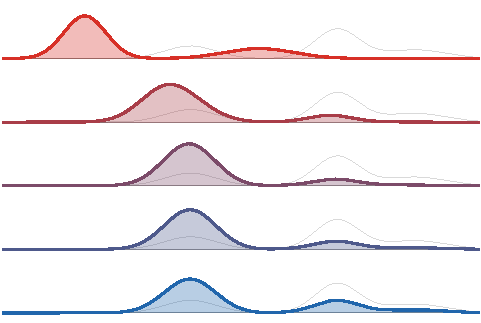
\includegraphics[width=.46\linewidth]{figures/gradflow-wfr-unbalanced-flow/balanced.pdf} &
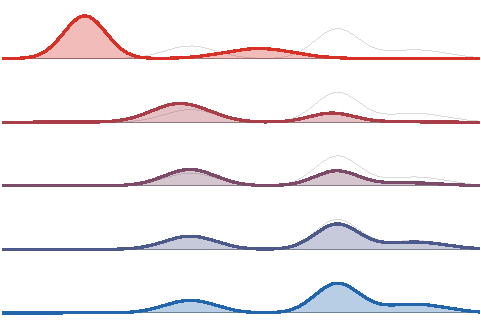
\includegraphics[width=.46\linewidth]{figures/gradflow-wfr-unbalanced-flow/unbalanced.pdf}
\end{tabular}
\caption{\emph{Balanced and unbalanced gradient flows of $\KL(\rho|\beta)$ for one-dimensional Gaussian mixtures.} In each panel the colored density stacks correspond to five increasing times, from red to blue, and the faint gray curve repeated on each row is the target mixture $\beta$. The balanced Wasserstein flow is the conservative Fokker--Planck equation, so mass must move through the low-density region between modes. The $\WFR_\kappa$ flow adds the birth--death reaction term in~\eqref{eq-wfr-kl-flow}; it attenuates overrepresented regions and creates missing mass near target modes, reaching the target shape much faster.}
\index{Wasserstein!gradient flow}% strictindex
\index{Wasserstein-Fisher-Rao}% strictindex
\index{birth-death dynamics}% strictindex
\index{Fokker-Planck equation}% strictindex
\label{fig:gradflow-wfr-unbalanced-flow}
\end{figure}

\subsection{Conditional Wasserstein Training of Infinite ResNets}
\index{conditional Wasserstein flow}% strictindex
\index{infinite ResNet}% strictindex
\label{sec-conditional-wasserstein-resnets}
\index{conditional optimal transport}% strictindex
\index{conditional Wasserstein distance}% strictindex
\index{ResNet}% strictindex
Residual networks learn small residual updates around the identity~\cite{HeZhangRenSun2016ResNet}. This makes depth behave like time: very deep residual architectures can be interpreted as discretizations of differential equations, a viewpoint developed in stable architectures, neural ODEs and mean-field optimal-control models of deep learning~\cite{HaberRuthotto2017StableArchitectures,LuZhongLiDong2018BeyondFiniteLayers,Chen2018NeuralODE,EHanLi2019MeanFieldDeepLearning}. The conditional-OT formulation of Barboni, Peyr\'e and Vialard~\cite{BarboniPeyreVialard2024ConditionalResNets} adds the width mean-field limit to this continuous-depth picture. It belongs to a broader conditional-transport literature, including fibered gradient flows~\cite{PeszekPoyato2023FiberedOptimalTransport}, conditional optimal transport on function spaces~\cite{HosseiniHsuTaghvaei2023ConditionalFunctionSpaces}, conditional Wasserstein distances for Bayesian OT flow matching~\cite{ChemseddineHagemannSteidlWald2024ConditionalWasserstein}, and dynamic conditional OT through simulation-free flows~\cite{KerriganMiglioriniSmyth2024DynamicConditionalOT}. From the viewpoint of Section~\ref{sec-generalized-dynamic-wasserstein-flows}, it is a concrete instance of a generalized dynamic Wasserstein flow: the conditional Wasserstein distance has a geodesic dynamic structure obtained by integrating the usual Benamou--Brenier action over the conditioning variable. The point of the construction is to keep track of two independent symmetries: neurons can be relabelled inside each layer, but mass should not move from one depth to another. Conditional Wasserstein geometry implements exactly this rule. It transports neurons fiber by fiber in parameter space, while the depth variable remains fixed.

We follow the three limiting levels of the model. A finite ResNet is first a labelled particle system arranged by layers. Sending the width to infinity turns each layer into a probability law of neurons. Sending the depth step to zero then turns the sequence of layer laws into a conditional measure indexed by depth, on which training becomes a Wasserstein gradient flow.

\paragraph{Finite-depth finite-width ResNets.}
\index{finite-depth ResNet}% strictindex
\index{finite-width ResNet}% strictindex
\index{residual block}% strictindex
The starting point is the ordinary architecture: depth is discrete, width is finite, and each layer carries a labelled collection of neurons. Fix a parameter space $\Theta\subset\RR^q$, a residual feature $\psi:\Theta\times\RR^d\to\RR^d$, a data law $\rho$ on input-label pairs $(z,y)$, and a loss $\ell$. With $L$ layers, step size $\tau=1/L$, widths $n_r$, and parameters $\theta_{r,i}\in\Theta$, a finite ResNet is the composition of the residual updates
\begin{equation}\label{eq-finite-resnet}
	z_{r+1}
	=
	z_r+\tau G_{r,n_r}(z_r),
	\qquad
	G_{r,n_r}(z)
	\eqdef
	\frac1{n_r}\sum_{i=1}^{n_r}\psi(\theta_{r,i},z),
	\qquad
	z_0=z,\qquad r=0,\ldots,L-1.
\end{equation}
The associated population loss, with $n=(n_0,\ldots,n_{L-1})$, is
\[
	f_{L,n}((\theta_{r,i})_{r,i})
	=
	\int \ell(z_L^{\theta}(z),y)\d\rho(z,y).
\]
Equivalently, each layer carries an empirical neuron law
\[
	\alpha_r
	=
	\frac1{n_r}\sum_{i=1}^{n_r}\delta_{\theta_{r,i}},
	\qquad
	G_{r,n_r}(z)
	=
	\int_\Theta\psi(\theta,z)\d\alpha_r(\theta).
\]
Thus a finite ResNet is already a discrete conditional measure on depth and neuron space,
\[
	\alpha^{L,n}(\d s,\d\theta)
	=
	\frac1L\sum_{r=0}^{L-1}\delta_{s_r}(\d s)\alpha_r(\d\theta),
	\qquad
	s_r=r/L,
\]
whose marginal on the depth variable is the discrete measure $\lambda_L=L^{-1}\sum_{r=0}^{L-1}\delta_{s_r}$.
\index{empirical measure}% strictindex
\index{neuron}% strictindex

\paragraph{Finite-depth mean-field limit.}
The first mean-field limit removes neuron labels inside each fixed layer. The residual depth grid stays discrete, but the widths tend to infinity. Each empirical law $\alpha_r$ is replaced by an arbitrary probability measure in $\Pp_2(\Theta)$, and each residual block becomes a mean-field residual block
\[
	z_{r+1}
	=
	z_r+\tau G_{\alpha_r}(z_r),
	\qquad z_0=z,
	\qquad
	G_{\alpha_r}(z)
	\eqdef
	\int_\Theta\psi(\theta,z)\d\alpha_r(\theta).
\]
The loss becomes a functional of the finite family of layer measures,
\[
	f_L(\alpha_0,\ldots,\alpha_{L-1})
	=
	\int \ell(z_L^\alpha(z),y)\d\rho(z,y).
\]
This is the finite-depth conditional Wasserstein setting with condition marginal $\lambda_L$: each fiber $s_r$ carries a Wasserstein geometry on neuron laws.

\paragraph{Continuous-depth conditional geometry.}
\index{continuous-depth ResNet}% strictindex
\index{depth variable}% strictindex
\index{conditional neuron law}% strictindex
The second limit turns the layer index into a conditioning variable. The model is no longer described by one neuron law, nor even by a finite list of them, but by a family of neuron laws indexed by depth. The state is therefore a conditional probability law
\[
	\alpha(\d s,\d\theta)=\alpha_s(\d\theta)\d s,
\]
or, equivalently, a probability measure on $[0,1]\times\Theta$ whose first marginal is Lebesgue measure. Here the condition is continuous depth, $s\in[0,1]$, the condition law is $\lambda(\d s)=\d s$, and the fiber space is the neuron parameter space $\Theta$. For two conditional neuron laws $\alpha(\d s,\d\theta)=\alpha_s(\d\theta)\d s$ and $\beta(\d s,\d\theta)=\beta_s(\d\theta)\d s$, the relevant distance is the depthwise quadratic Wasserstein metric
\begin{equation}\label{eq-resnet-depth-wasserstein}
	\Wass_{2,\lambda}^2(\alpha,\beta)
	=
	\int_0^1\Wass_2^2(\alpha_s,\beta_s)\d s.
\end{equation}
It compares neurons only at the same depth: transport in $\theta$ is allowed fiber by fiber, while mass is not transported between layers.

\paragraph{Infinite-depth mean-field ResNet.}
Once depth is continuous, the forward pass is a controlled ODE and the control is the conditional neuron law. A mean-field infinite-depth and infinite-width ResNet is described by a measurable family $s\mapsto\alpha_s\in\Pp_2(\Theta)$. Each slice is the neuron law of one infinitesimal residual block, and the feature $\psi(\theta,z)$ now acts as a vector field on the state variable. The forward pass is
\begin{equation}\label{eq-mean-field-resnet-forward}
	\partial_s z_s
	=
	G_{\alpha_s}(z_s)
	\eqdef
	\int_\Theta \psi(\theta,z_s)\d\alpha_s(\theta),
	\qquad z_0=z.
\end{equation}
The population risk is
\[
	f_{\mathrm{Res}}(\alpha)
	=
	\int \ell(z_1^\alpha(z),y)\d\rho(z,y).
\]
Under the usual regularity assumptions ensuring well-posedness of the ODE, this defines a functional on the conditional Wasserstein space.

\paragraph{Conditional Wasserstein gradient flow.}
\index{layerwise matching}% strictindex
\index{conditional gradient flow}% strictindex
Training is now steepest descent for an objective on conditional laws. More generally, let $F$ be a differentiable functional on measures $\alpha(\d s,\d\theta)=\alpha_s(\d\theta)\lambda(\d s)$ with fixed first marginal $\lambda$. For signed perturbations $\xi(\d s,\d\theta)=\xi_s(\d\theta)\lambda(\d s)$ satisfying $\int_\Theta\d\xi_s=0$ for $\lambda$-a.e. $s$, we use the fiberwise first-variation convention
\[
	\frac{\d}{\d\varepsilon}F(\alpha+\varepsilon\xi)\bigg|_{\varepsilon=0}
	=
	\int_S\int_\Theta \frac{\delta F}{\delta\alpha_s}(\alpha)(\theta)\d\xi_s(\theta)\d\lambda(s).
\]
The formal conditional Wasserstein gradient flow is the family of continuity equations
\begin{equation}\label{eq-conditional-resnet-gradient-flow}
	\partial_t\alpha_{t,s}
	+\diverg_\theta(\alpha_{t,s}v_{t,s})=0,
	\qquad
	v_{t,s}(\theta)
	=
	-\nabla_\theta\frac{\delta F}{\delta\alpha_s}(\alpha_t)(\theta),
\end{equation}
for $\lambda$-a.e. condition $s$, whenever the first variation is differentiable in the parameter variable. In the ResNet case one takes $F=f_{\mathrm{Res}}$. The equation is fiberwise in its transport geometry, but not decoupled as a training dynamics: changing $\alpha_s$ affects the terminal loss through the forward ODE and the corresponding adjoint equation. Thus each depth performs a Wasserstein steepest descent in its own neuron space, while all depths interact through the state trajectory.
\index{first variation}% strictindex
\index{Wasserstein!gradient flow}% strictindex

\paragraph{Particle discretization and layerwise matching.}
The finite network is recovered by discretizing both the condition variable and the fiber measures. With the discrete depth marginal $\lambda_L$, finite-depth finite-width ResNets are particle approximations of the conditional flow above. If two networks have the same depth grid and the same widths, and if their empirical layer laws are
\[
	\alpha_r=\frac1{n_r}\sum_{i=1}^{n_r}\delta_{\theta_{r,i}},
	\qquad
	\beta_r=\frac1{n_r}\sum_{i=1}^{n_r}\delta_{\theta'_{r,i}},
\]
then their squared conditional distance is
\[
	\Wass_{2,\lambda_L}^2(\alpha^{L,n},\beta^{L,n})
	=
	\frac1L\sum_{r=0}^{L-1} \Wass_2^2(\alpha_r,\beta_r).
\]
Keeping neuron labels fixed gives the labelled parameter distance
\[
	\frac1L\sum_{r=0}^{L-1}\frac1{n_r}
	\sum_{i=1}^{n_r}\norm{\theta_{r,i}-\theta'_{r,i}}^2,
\]
which corresponds to a particular feasible coupling and therefore upper bounds the squared conditional Wasserstein distance. Optimizing over permutations inside each equal-weight layer gives the Wasserstein matching term above. In this sense, the shallow mean-field flow is the one-fiber case, whereas infinitely deep ResNets require a continuum of Wasserstein flows indexed by depth and coupled through the network state.
\index{continuous depth}% strictindex
\index{residual network}% strictindex
\index{mean-field neural network}% strictindex
\index{Wasserstein!gradient flow}% strictindex

\subsection{Second-Order Momentum Flows}
\label{sec-second-order-momentum-flows}
\index{momentum flow}% strictindex
\index{second-order flow}% strictindex
\index{particle Wasserstein descent}% strictindex

The minimizing-movement viewpoint is intrinsically first order: a JKO step produces the next measure by trading off proximity to the previous measure and decrease of the energy. Momentum adds a memory of velocity. The state is therefore no longer only a measure, but a measure together with a tangent, or equivalently phase-space, variable. This makes a direct implicit JKO construction less natural than for first-order flows. We instead use an explicit construction, in the same spirit as optimization and machine-learning practice: momentum reduces zig-zagging across stiff directions, helps iterates keep a coherent direction through shallow valleys, and can accelerate convergence when the geometry is favorable~\cite{Qian1999Momentum,Sutskever2013Momentum}. The goal is to write this inertial idea in a form compatible with Wasserstein particle flows.
\index{JKO scheme}% strictindex
\index{explicit Euler scheme}% strictindex

\paragraph{Finite-dimensional momentum.}
\index{Polyak momentum}% strictindex
\index{Nesterov acceleration}% strictindex
\index{heavy-ball method}% strictindex
Let $F:\RR^{N}\to\RR$ be a smooth finite-dimensional objective. Polyak's heavy-ball method~\cite{Polyak1964HeavyBall} augments gradient descent with a velocity variable. With step size $h>0$ and damping $\gamma>0$, one convenient velocity form is
\begin{equation}\label{eq-polyak-momentum}
	S^{k+1}=(1-\gamma h)S^k-h\nabla F(X^k),
	\qquad
	X^{k+1}=X^k+hS^{k+1}.
\end{equation}
If $S^k$ approximates $\dot X(kh)$, this is the explicit Euler discretization of the first-order system
\begin{equation}\label{eq-heavy-ball-first-order-system}
	\dot X(t)=S(t),
	\qquad
	\dot S(t)=-\gamma S(t)-\nabla F(X(t)),
\end{equation}
or equivalently the damped second-order equation
\begin{equation}\label{eq-heavy-ball-ode}
	\ddot X(t)+\gamma\dot X(t)+\nabla F(X(t))=0.
\end{equation}
Nesterov's accelerated method~\cite{Nesterov1983Accelerated} uses a closely related extrapolation but evaluates the gradient at a look-ahead point,
\index{look-ahead point}% strictindex
\begin{equation}\label{eq-nesterov-momentum}
	Y^k=X^k+\theta_k(X^k-X^{k-1}),
	\qquad
	X^{k+1}=Y^k-h\nabla F(Y^k),
\end{equation}
with $\theta_k=(k-1)/(k+r-1)$ for the classical convex schedule $r=3$. Its scaling limit is the time-dependent damping equation
\begin{equation}\label{eq-nesterov-ode}
	\ddot X(t)+\frac{r}{t}\dot X(t)+\nabla F(X(t))=0.
\end{equation}
This ODE interpretation is due to Su, Boyd and Cand{\`e}s~\cite{SuBoydCandes2016ODE}; see also the variational perspective of Wibisono, Wilson and Jordan~\cite{WibisonoWilsonJordan2016Acceleration}, and the inertial dynamics with Hessian-driven damping studied by Attouch, Peypouquet and Redont~\cite{AttouchPeypouquetRedont2016HessianDamping}. High-resolution ODE limits refine this picture by keeping terms that distinguish heavy-ball and Nesterov dynamics beyond their leading continuous-time behavior~\cite{ShiDuJordanSu2018HighResolution}. For the Wasserstein extension below, the autonomous heavy-ball form \eqref{eq-heavy-ball-first-order-system} is the cleanest template.
\index{heavy-ball method}% strictindex
\index{damped second-order equation}% strictindex
\index{ODE limit}% strictindex

\paragraph{Empirical Wasserstein lift.}
\index{Wasserstein gradient}% strictindex
\index{empirical!measure}% strictindex
\index{empirical Wasserstein metric}% strictindex
We now take a functional $f$ on measures and lift it to particle configurations. For $X=(x_1,\ldots,x_n)\in(\RR^d)^n$, write
\begin{equation}\label{eq-empirical-momentum-lift}
	\al_X \eqdef \frac1n\sum_{i=1}^n \delta_{x_i},
	\qquad
	F(X) \eqdef f(\al_X).
\end{equation}
This is the same empirical lift as in \eqref{eq:wassflows-particles}, and is the particle viewpoint underlying mean-field analyses of wide neural networks and Wasserstein gradient methods~\cite{ChizatBach2018OverparameterizedOT,MeiMontanariNguyen2018MeanFieldNN,RotskoffVandenEijnden2018Trainability}. The important point is that the configuration space is not used with the plain Euclidean metric, but with the empirical metric
\[
	\norm{\dot X}_n^2
	\eqdef
	\frac1n\sum_{i=1}^n\norm{\dot x_i}^2,
\]
which is the metric induced by $\Wass_2$ on equally weighted empirical measures with fixed labels. Moving only $x_i$ to $x_i+\varepsilon \xi$ gives
\[
	\left.\frac{\d}{\d\varepsilon}\right|_{\varepsilon=0}
	F(x_1,\ldots,x_i+\varepsilon\xi,\ldots,x_n)
	=
	\frac1n\dotp{\nabla\delta f(\al_X)(x_i)}{\xi}.
\]
Thus, if $\nabla^{(n)}F$ denotes the gradient for the metric $\norm{\cdot}_n$, then
\begin{equation}\label{eq-empirical-lift-gradient}
	(\nabla^{(n)}F(X))_i
	=
	n\nabla_{x_i}F(X)
	=
	\nabla\delta f(\al_X)(x_i)
	=
	\Wgrad f(\al_X)(x_i).
\end{equation}
The first-order Wasserstein particle descent is therefore $\dot x_i=v_{\al_X}(x_i)$ with
\begin{equation}\label{eq-momentum-wasserstein-velocity}
	v_\al(x)\eqdef -\Wgrad f(\al)(x)=-\nabla\delta f(\al)(x).
\end{equation}
Applying the heavy-ball equation to the empirical metric gives the second-order Wasserstein momentum system
\begin{equation}\label{eq-wasserstein-momentum-particles}
	\dot x_i(t)=s_i(t),
	\qquad
	\dot s_i(t)=-\gamma s_i(t)+v_{\al_t}(x_i(t)),
	\qquad
	\al_t=\frac1n\sum_{i=1}^n\delta_{x_i(t)} .
\end{equation}
Equivalently,
\[
	\ddot x_i(t)+\gamma\dot x_i(t)
	=
	v_{\al_t}(x_i(t))
	=
	-\Wgrad f(\al_t)(x_i(t)).
\]
This is an explicit inertial particle method for the measure energy $f$: the Wasserstein steepest-descent field acts as an acceleration rather than as an instantaneous velocity. The statement is deliberately formal at this level; rigorous mean-field limits require stability and regularity assumptions on $v_\al$, as in propagation-of-chaos arguments for classical Vlasov dynamics and in mean-field analyses of interacting learning systems.
\index{inertial particle method}% strictindex
\index{mean-field momentum}% strictindex

\begin{prop}[Discrete mechanical energy dissipation]\label{prop-second-order-energy-dissipation}
\index{mechanical energy}% strictindex
\index{energy!dissipation}% strictindex
	Assume that $f$ and the particle solution are smooth enough to justify differentiating the identities above along \eqref{eq-wasserstein-momentum-particles}. Define
	\[
		\mathcal H_n(X,S)
		\eqdef
		F(X)+\frac1{2n}\sum_{i=1}^n\norm{s_i}^2,
		\qquad
		S=(s_1,\ldots,s_n).
	\]
	Then along \eqref{eq-wasserstein-momentum-particles},
	\begin{equation}\label{eq-second-order-energy-dissipation}
		\frac{\d}{\d t}\mathcal H_n(X(t),S(t))
		=
		-\frac{\gamma}{n}\sum_{i=1}^n\norm{s_i(t)}^2
		\leq 0 .
	\end{equation}
\end{prop}
\begin{proof}
	By \eqref{eq-empirical-lift-gradient} and the definition $v_\al=-\Wgrad f(\al)$, one has $\nabla_{x_i}F(X)=-v_{\al_X}(x_i)/n$. Hence
	\[
		\frac{\d}{\d t}F(X(t))
		=
		\sum_{i=1}^n \dotp{\nabla_{x_i}F(X(t))}{s_i(t)}
		=
		-\frac1n\sum_{i=1}^n\dotp{v_{\al_t}(x_i(t))}{s_i(t)}.
	\]
	On the other hand,
	\[
		\frac{\d}{\d t}\frac1{2n}\sum_i\norm{s_i(t)}^2
		=
		\frac1n\sum_i\dotp{s_i(t)}{-\gamma s_i(t)+v_{\al_t}(x_i(t))}.
	\]
	The force terms cancel, leaving \eqref{eq-second-order-energy-dissipation}.
\end{proof}
The identity says that friction dissipates exactly the kinetic part of the mechanical energy. In the undamped case $\gamma=0$, the same computation gives conservation of $\mathcal H_n$.

\paragraph{Phase-space formulation.}
\index{phase-space flow}% strictindex
\index{Lagrangian velocity}% strictindex
\index{phase space}% strictindex
Because momentum is part of the state, the mean-field object is not merely a measure on positions. It is a law on phase space $(x,s)$, whose spatial marginal is the current distribution of particles. Here $s$ is a Lagrangian particle velocity; it should not be confused with the Eulerian momentum measure $m=\rho v$ used in the Benamou--Brenier convex formulation~\eqref{eq:benamou-brenier-convex}. The particle ODE then becomes a transport equation in phase space. This is the deterministic analogue of the kinetic mean-field viewpoint used for interacting particle systems; in learning, heavy-ball mean-field limits have recently been used to analyze wide networks trained with momentum~\cite{WuKungurtsevMondelli2022HeavyBallMeanField}.
\index{phase-space measure}% strictindex
\index{kinetic mean-field limit}% strictindex
\index{heavy-ball method}% strictindex

\begin{prop}[Phase-space Liouville formulation]\label{prop-second-order-liouville}
\index{Liouville equation}% strictindex
\index{phase space}% strictindex
\index{phase-space measure}% strictindex
	Let $v_\al$ be smooth enough that \eqref{eq-wasserstein-momentum-particles} has a classical solution. Define the empirical phase-space measure
	\[
		\eta_t^n \eqdef \frac1n\sum_{i=1}^n\delta_{(x_i(t),s_i(t))}
		\in \Pp(\RR^d_x\times\RR^d_s),
		\qquad
		\al_t^n=(\pi_x)_\sharp\eta_t^n .
	\]
	Then $\eta_t^n$ solves, in the sense of distributions,
	\begin{equation}\label{eq-second-order-liouville-empirical}
		\partial_t\eta_t^n
		+
		\nabla_x\cdot(s\,\eta_t^n)
		+
		\nabla_s\cdot\bigl((-\gamma s+v_{\al_t^n}(x))\,\eta_t^n\bigr)
		=0 .
	\end{equation}
	If, as $n\to\infty$, the empirical phase-space laws converge to a smooth density $\eta_t(x,s)$ and the nonlinear fields converge accordingly, the limiting kinetic equation is
	\begin{equation}\label{eq-second-order-liouville-density}
		\partial_t\eta_t
		+
		\nabla_x\cdot(s\,\eta_t)
		+
		\nabla_s\cdot\bigl((-\gamma s+v_{\al_t}(x))\,\eta_t\bigr)
		=0,
		\qquad
		\al_t=(\pi_x)_\sharp\eta_t .
	\end{equation}
\end{prop}
\begin{proof}
	Let $\varphi\in C_c^\infty(\RR^d_x\times\RR^d_s)$. Along the particle system,
	\[
		\frac{\d}{\d t}
		\int \varphi\,\d\eta_t^n
		=
		\frac1n\sum_{i=1}^n
		\left[
		\dotp{\nabla_x\varphi(x_i,s_i)}{s_i}
		+
		\dotp{\nabla_s\varphi(x_i,s_i)}{-\gamma s_i+v_{\al_t^n}(x_i)}
		\right].
	\]
	Rewriting the right-hand side as an integral against $\eta_t^n$ and integrating by parts gives \eqref{eq-second-order-liouville-empirical}. Passing formally to the mean-field limit gives \eqref{eq-second-order-liouville-density}.
\end{proof}

\begin{rem}[Newtonian limit]\label{rem-newtonian-momentum-limit}
\index{Newtonian dynamics}% strictindex
\index{Newton dynamics}% strictindex
\index{inertia}% strictindex
	If damping is removed, or if inertia dominates friction after rescaling, \eqref{eq-wasserstein-momentum-particles} becomes
	\[
		\ddot x_i(t)=v_{\al_t}(x_i(t)).
	\]
	This is Newton's law with acceleration field $v_{\al_t}$. Thus first-order Wasserstein gradient flow reads the force as a velocity, while second-order momentum flow reads the same force as an acceleration. The price is that the state is no longer just the spatial measure $\al_t$; it is the phase-space law of position and velocity. In this limit the flow is Hamiltonian rather than dissipative whenever the force comes from a smooth interaction energy and $\gamma=0$.
\end{rem}

\begin{example}[Quadratic energies and gravitational attraction]\label{ex-quadratic-momentum-gravity}
\index{quadratic energy}% strictindex
\index{interaction kernel}% strictindex
\index{gravity interaction}% strictindex
	The quadratic-plus-linear energies
	\[
		f(\al)=\frac12\iint k(x,y)\,\d\al(x)\d\al(y)+\int V(x)\,\d\al(x),
		\qquad k(x,y)=k(y,x),
	\]
	are the interaction energies already discussed around \eqref{eq:quadratic-func}, up to the harmless convention of inserting the factor $1/2$. The force computed there becomes, in the present inertial setting, an acceleration:
	\[
		v_\al(x)
		=
		-\int \nabla_x k(x,y)\,\d\al(y)-\nabla V(x).
	\]
	For the attractive Newtonian kernel in three dimensions, $k(x,y)=-G/\norm{x-y}$, understood with a short-distance regularization if needed, this gives
	\[
		v_\al(x)
		=
		G\int \frac{y-x}{\norm{x-y}^3}\,\d\al(y)-\nabla V(x),
	\]
	the usual mean-field gravitational acceleration. The phase-space equation \eqref{eq-second-order-liouville-density} is then a damped Vlasov-type equation. This kinetic viewpoint is classical in statistical physics: Boltzmann introduced the description of gases through phase-space distributions, the collisionless mean-field limit gives Liouville--Vlasov equations, and adding collision operators leads to the Boltzmann equation~\cite{CercignaniIllnerPulvirenti1994DiluteGases,Villani2002Boltzmann,BraunHepp1977Vlasov}.
	\index{Vlasov equation}% strictindex
	\index{Boltzmann equation}% strictindex
	\index{kinetic equation}% strictindex
\end{example}

The numerical illustration below uses the energy-distance kernel
\index{energy distance}% strictindex
\index{maximum mean discrepancy}% strictindex
\[
	k(x,y)=-\norm{x-y},
	\qquad
	f(\al)=\MMD_k^2(\al,\beta)
	=
	\iint k(x,y)\,\d(\al-\beta)(x)\d(\al-\beta)(y).
\]
This is the usual squared energy distance between $\al$ and $\beta$. Away from the diagonal, its Wasserstein velocity is
\[
	v_\al(x)
	=
	2\int \frac{x-y}{\norm{x-y}}\,\d(\al-\beta)(y).
\]
For numerical stability, Figure~\ref{fig:gradflow-second-order-momentum-mmd} uses the smoothed distance $\sqrt{\norm{x-y}^2+\delta^2}$ with a small $\delta$. It compares the first-order flow with the undamped Newton lift $\ddot x=v_{\al_t}(x)=-\nabla_W f(\al_t)(x)$, initialized with zero velocity. The initial measure is a single Gaussian located to the left of a two-Gaussian target mixture. Both the transported measure and the target are discretized by large empirical clouds, and the smooth density views are KDE renderings of these particles. The trajectory panels display only a representative subset of initial particles selected by farthest-point sampling.
\index{kernel density estimate}% strictindex
\index{farthest-point sampling}% strictindex

\begin{figure}[H]
\centering
\def\mmdmomentumpanelheight{.128\linewidth}
\newcommand{\mmdmomentumrowlabel}[1]{\makebox[.017\linewidth][c]{\raisebox{-.5\height}{\rotatebox[origin=c]{90}{\scriptsize #1}}}}
\newcommand{\mmdmomentumpanel}[1]{\raisebox{-.5\height}{\includegraphics[height=\mmdmomentumpanelheight]{#1}}}
\begin{tabular}{@{}c@{\hspace{.003\linewidth}}c@{\hspace{.004\linewidth}}c@{\hspace{.004\linewidth}}c@{\hspace{.004\linewidth}}c@{\hspace{.004\linewidth}}c@{\hspace{.004\linewidth}}c@{}}
&
\scriptsize trajectories
&
\scriptsize $t=0$
&
\scriptsize $t=.05$
&
\scriptsize $t=.14$
&
\scriptsize $t=.36$
&
\scriptsize $t=1$\\[-.25em]
\mmdmomentumrowlabel{GF}
&
\mmdmomentumpanel{figures/gradflow-second-order-momentum-mmd/first-trajectories.pdf}
&
\mmdmomentumpanel{figures/gradflow-second-order-momentum-mmd/first-density-t000.pdf}
&
\mmdmomentumpanel{figures/gradflow-second-order-momentum-mmd/first-density-t005.pdf}
&
\mmdmomentumpanel{figures/gradflow-second-order-momentum-mmd/first-density-t014.pdf}
&
\mmdmomentumpanel{figures/gradflow-second-order-momentum-mmd/first-density-t036.pdf}
&
\mmdmomentumpanel{figures/gradflow-second-order-momentum-mmd/first-density-t100.pdf}\\[-.15em]
\mmdmomentumrowlabel{Newton}
&
\mmdmomentumpanel{figures/gradflow-second-order-momentum-mmd/newton-trajectories.pdf}
&
\mmdmomentumpanel{figures/gradflow-second-order-momentum-mmd/newton-density-t000.pdf}
&
\mmdmomentumpanel{figures/gradflow-second-order-momentum-mmd/newton-density-t005.pdf}
&
\mmdmomentumpanel{figures/gradflow-second-order-momentum-mmd/newton-density-t014.pdf}
&
\mmdmomentumpanel{figures/gradflow-second-order-momentum-mmd/newton-density-t036.pdf}
&
\mmdmomentumpanel{figures/gradflow-second-order-momentum-mmd/newton-density-t100.pdf}
\end{tabular}
\caption{\emph{First-order and Newton Wasserstein particle flows for the squared MMD with the energy-distance kernel $k(x,y)=-\norm{x-y}$.} The first row follows the overdamped Wasserstein gradient flow. The second row follows the infinite-momentum Newton dynamics $\ddot x=-\nabla_W f(\al_t)(x)$, so the same Wasserstein force is read as an acceleration rather than a velocity. Both rows use the same large empirical source cloud and the same empirical two-Gaussian target cloud. Dashed gray contours show a KDE of the target particles, colored panels show KDEs of the evolving transported particles, and the left panels show farthest-point-subsampled trajectories.}
\label{fig:gradflow-second-order-momentum-mmd}
\end{figure}


\paragraph{Entropy without an empirical energy.}
\index{entropy closure}% strictindex
\index{density closure}% strictindex
\index{empirical energy}% strictindex
\index{entropy score}% strictindex
The previous interaction example has a genuine value on empirical measures: once the particles are known, the double sum approximates the interaction energy. Entropy gives the complementary situation. Its Wasserstein gradient flow is the simplest diffusion equation, but the entropy itself is finite only on absolutely continuous measures. A particle method must therefore introduce a density, or score, closure before the inertial template can be applied.

\begin{example}[Entropy-driven inertial flow]\label{ex-second-order-entropy-score}
\index{Shannon entropy}% strictindex
\index{score function}% strictindex
\index{KDE score}% strictindex
\index{phase-space equation}% strictindex
	Let
	\[
		f(\al)=
		\begin{cases}
			\displaystyle \int_{\RR^d} \rho(x)\log\rho(x)\,\d x,
			& \text{if } \al=\rho\d x,\\[.4em]
			+\infty, & \text{otherwise.}
		\end{cases}
	\]
	Thus $f(\al_X)=+\infty$ for an empirical measure $\al_X=n^{-1}\sum_i\delta_{x_i}$, and the finite-dimensional lift $F(X)=f(\al_X)$ is not meaningful. For $\al=\rho\d x$ with a smooth positive density, however,
	\[
		\delta f(\al)(x)=\log\rho(x)+1,
			\qquad
		v_\al(x)=-\nabla\log\rho(x).
	\]
	The first-order Wasserstein gradient flow is therefore the heat equation $\partial_t\rho_t=\Delta\rho_t$. If the spatial marginal remains smooth and positive, the corresponding formal second-order phase-space equation is
\index{heat equation}% strictindex
\index{phase-space equation}% strictindex
	\begin{equation}\label{eq-second-order-entropy-phase-space}
		\partial_t\eta_t
		+
		\nabla_x\cdot(s\eta_t)
		+
		\nabla_s\cdot\bigl((-\gamma s-\nabla\log\rho_t(x))\eta_t\bigr)
		=0,
		\qquad
		\rho_t(x)=\int_{\RR^d}\eta_t(x,s)\,\d s .
	\end{equation}
	This is a kinetic, inertial version of entropy diffusion: the entropy score acts as an acceleration rather than as an instantaneous velocity.
	\end{example}

For the numerical illustration, we add the quadratic confinement $V(x)=\norm{x}^2/2$. In one dimension the overdamped equation becomes the Ornstein--Uhlenbeck Fokker--Planck equation
\index{quadratic confinement}% strictindex
\index{Ornstein-Uhlenbeck process}% strictindex
\[
\partial_t\rho_t=\partial_{xx}\rho_t+\partial_x(x\rho_t),
\]
whose stationary law is the centered Gaussian $\mathcal N(0,1)$. The Newton lift is discretized directly in phase space: for a density $\eta_t(x,s)$ with spatial marginal $\rho_t(x)=\int\eta_t(x,s)\,\d s$, it reads
\[
\partial_t\eta_t+\partial_x(s\eta_t)+\partial_s\bigl((-\partial_x\log\rho_t(x)-x)\eta_t\bigr)=0.
\]
Both equations are solved by finite differences on fixed grids, with a mild grid smoothing only to evaluate the logarithmic derivative in the Newton row. The first row of Figure~\ref{fig:gradflow-second-order-momentum-entropy} shows only the spatial density of the Wasserstein gradient flow. The second and third rows show, for the Newton equation, respectively the spatial marginal and the full phase-space density; the latter uses white for zero mass and black for high mass.
\index{finite difference scheme}% strictindex
\index{phase-space density}% strictindex

\begin{figure}[H]
\centering
\newcommand{\entropyclosurespatialheight}{.088\linewidth}
\newcommand{\entropyclosurephaseheight}{.101\linewidth}
\newcommand{\entropyclosurerowlabel}[2]{\makebox[.018\linewidth][c]{\raisebox{-.5\height}{\rotatebox[origin=c]{90}{\small #2}}}}
\newcommand{\entropyclosurepanel}[2]{\raisebox{-.5\height}{\includegraphics[height=#1]{#2}}}
\begin{tabular}{@{}c@{\hspace{.006\linewidth}}c@{\hspace{.004\linewidth}}c@{\hspace{.004\linewidth}}c@{\hspace{.004\linewidth}}c@{\hspace{.004\linewidth}}c@{\hspace{.004\linewidth}}c@{}}
& \small $t=0$ & \small $t=.05$ & \small $t=.12$ & \small $t=.24$ & \small $t=.4$ & \small $t=.6$\\[-.25em]
\entropyclosurerowlabel{\entropyclosurespatialheight}{GF}
& \entropyclosurepanel{\entropyclosurespatialheight}{figures/gradflow-second-order-momentum-entropy/gf-spatial-t00.pdf}
& \entropyclosurepanel{\entropyclosurespatialheight}{figures/gradflow-second-order-momentum-entropy/gf-spatial-t01.pdf}
& \entropyclosurepanel{\entropyclosurespatialheight}{figures/gradflow-second-order-momentum-entropy/gf-spatial-t02.pdf}
& \entropyclosurepanel{\entropyclosurespatialheight}{figures/gradflow-second-order-momentum-entropy/gf-spatial-t03.pdf}
& \entropyclosurepanel{\entropyclosurespatialheight}{figures/gradflow-second-order-momentum-entropy/gf-spatial-t04.pdf}
& \entropyclosurepanel{\entropyclosurespatialheight}{figures/gradflow-second-order-momentum-entropy/gf-spatial-t05.pdf}\\[.18em]
\entropyclosurerowlabel{\entropyclosurespatialheight}{Newton}
& \entropyclosurepanel{\entropyclosurespatialheight}{figures/gradflow-second-order-momentum-entropy/newton-spatial-t00.pdf}
& \entropyclosurepanel{\entropyclosurespatialheight}{figures/gradflow-second-order-momentum-entropy/newton-spatial-t01.pdf}
& \entropyclosurepanel{\entropyclosurespatialheight}{figures/gradflow-second-order-momentum-entropy/newton-spatial-t02.pdf}
& \entropyclosurepanel{\entropyclosurespatialheight}{figures/gradflow-second-order-momentum-entropy/newton-spatial-t03.pdf}
& \entropyclosurepanel{\entropyclosurespatialheight}{figures/gradflow-second-order-momentum-entropy/newton-spatial-t04.pdf}
& \entropyclosurepanel{\entropyclosurespatialheight}{figures/gradflow-second-order-momentum-entropy/newton-spatial-t05.pdf}\\[.18em]
\entropyclosurerowlabel{\entropyclosurephaseheight}{Phase}
& \entropyclosurepanel{\entropyclosurephaseheight}{figures/gradflow-second-order-momentum-entropy/newton-phase-t00.pdf}
& \entropyclosurepanel{\entropyclosurephaseheight}{figures/gradflow-second-order-momentum-entropy/newton-phase-t01.pdf}
& \entropyclosurepanel{\entropyclosurephaseheight}{figures/gradflow-second-order-momentum-entropy/newton-phase-t02.pdf}
& \entropyclosurepanel{\entropyclosurephaseheight}{figures/gradflow-second-order-momentum-entropy/newton-phase-t03.pdf}
& \entropyclosurepanel{\entropyclosurephaseheight}{figures/gradflow-second-order-momentum-entropy/newton-phase-t04.pdf}
& \entropyclosurepanel{\entropyclosurephaseheight}{figures/gradflow-second-order-momentum-entropy/newton-phase-t05.pdf}
\end{tabular}
\caption{\emph{Finite-difference entropy and inertial entropy flows in one dimension.} The initial spatial density is a three-Gaussian mixture with different widths and overlapping components. The top row solves the confined entropy Wasserstein gradient flow, i.e. the OU/Fokker--Planck equation, whose stationary density is the dashed centered Gaussian. The two lower rows solve the undamped Newton lift on a grid in $(x,s)$, initialized with a narrow centered speed distribution: its spatial marginal is shown in color and the full phase-space density below in grayscale.}
\label{fig:gradflow-second-order-momentum-entropy}
\end{figure}
